\section{Additional experimental details}
\label{sec:supp_details}

% Generated by analysis/v77_model_arch.py; all counts in billions.
\begin{table}[!htbp]\normalfont
\centering
\small
\setlength{\tabcolsep}{3pt}
\begin{tabular*}{\textwidth}{@{\extracolsep{\fill}}llrrrrr@{}}
\toprule
Model & Class and type & $N_{\rm meta}$ & $N_{\rm active}$ & $N_{\rm unique}$ & $N_{0,\rm matrix}$ & Convention \\
\midrule
\multicolumn{7}{l}{\textit{Original heterogeneous panel (12 models)}} \\
Gemma-3-270M & G3; dense & 0.436 & 0.436 & 0.268 & 0.100 & M, U, T \\
Gemma-3-1B & G3; dense & 1.302 & 1.302 & 1.000 & 0.698 & M, U, T \\
Gemma-3-4B & G3; dense & 4.552 & 4.552 & 3.880 & 3.209 & M, U, T \\
Gemma-3-12B & G3; dense & 12.773 & 12.773 & 11.766 & 10.758 & M, U, T \\
Gemma-3-27B & G3; dense & 28.419 & 28.419 & 27.009 & 25.598 & M, U, T \\
Gemma-4-31B & G4; dense & 32.107 & 32.107 & 30.697 & 29.287 & M, U, T \\
Muse-30B & MG; dense & 27.855 & 27.855 & 27.855 & 25.164 & M, U, T \\
OLMo-3-7B & O3; dense & 7.298 & 7.298 & 7.298 & 6.476 & M, U, T \\
OLMo-3-32B & O3; dense & 32.234 & 32.234 & 32.234 & 31.206 & M, U, T \\
Qwen3-0.6B & Q3; dense & 0.752 & 0.752 & 0.596 & 0.440 & M, U, T \\
Qwen3-1.7B & Q3; dense & 2.032 & 2.032 & 1.721 & 1.409 & M, U, T \\
Qwen3-4B & Q3; dense & 4.411 & 4.411 & 4.022 & 3.633 & M, U, T \\
\midrule
\multicolumn{7}{l}{\textit{Pythia architecture sizes (revisions audited separately)}} \\
Pythia-160M & PN; dense & 0.162 & 0.162 & 0.162 & 0.085 & M, U, T \\
Pythia-410M & PN; dense & 0.405 & 0.405 & 0.405 & 0.302 & M, U, T \\
Pythia-1B & PN; dense & 1.012 & 1.012 & 1.012 & 0.805 & M, U, T \\
Pythia-1.4B & PN; dense & 1.415 & 1.415 & 1.415 & 1.208 & M, U, T \\
Pythia-2.8B & PN; dense & 2.775 & 2.775 & 2.775 & 2.517 & M, U, T \\
Pythia-6.9B & PN; dense & 6.857 & 6.857 & 6.857 & 6.442 & M, U, T \\
\midrule
\multicolumn{7}{l}{\textit{Later prospective additions}} \\
Qwen3-8B & Q3; dense & 8.191 & 8.191 & 8.191 & 6.946 & M, U, T \\
Qwen3-14B & Q3; dense & 14.768 & 14.768 & 14.768 & 13.212 & M, U, T \\
\bottomrule
\end{tabular*}
\caption{The table lists cached text-model architectures and parameter counts ($10^9$). M is the literal meta-device parameter count before restoring tied weights, U the unique parameter count after restoring ties, and T the transformer matrices, excluding embeddings, language-model head, norms and biases. Dense active counts equal M under this convention; all 12 original panel models are dense. M can double-count a tied embedding and output head. Pythia T equals the law covariate $L(4h^2+2hm)$. Multimodal checkpoints use their text decoder only. The class abbreviations are G3 for Gemma3ForCausalLM, G4 for Gemma4ForCausalLM, MG for MuseGlimmerTextModel with a language-model head, O3 for Olmo3ForCausalLM, PN for GPTNeoXForCausalLM, and Q3 for Qwen3ForCausalLM. The cached top-level classes for multimodal Gemma and Muse are the corresponding ForConditionalGeneration classes. The frozen Gemma-3 student counts are 0.435870336B, 1.301875840B, and 4.971331952B; the last includes 0.419816304B non-text parameters and differs from the text-only M column. Gemma-4-26B-A4B-it is a cached MoE outside the registry and panel and is excluded here. Rows identify models within each cohort; columns give the architecture class and parameter-count conventions. This is a \mbox{post-hoc} architecture audit. MoE means mixture of experts.}
\label{tab:model_arch}
\end{table}


\FloatBarrier

\section{Alternative functional forms and model selection}
\label{sec:supp_forms}

\subsection{Pruning: expanded development set and the selection rule}
Table~\ref{tab:v53_loso} reports the leave-one-source-out comparison of the pruning candidates on the
expanded seventeen-state development set, under the pre-committed rule that selected the delivered
form.
\begin{table}[tb]\normalfont\centering\footnotesize
\begin{tabular*}{\textwidth}{@{\extracolsep{\fill}}>{\raggedright\arraybackslash\hspace{0pt}}p{\dimexpr 0.200000000\textwidth-2.000000000\tabcolsep\relax}>{\raggedright\arraybackslash\hspace{0pt}}p{\dimexpr 0.270000000\textwidth-2.700000000\tabcolsep\relax}>{\raggedright\arraybackslash\hspace{0pt}}p{\dimexpr 0.130000000\textwidth-1.300000000\tabcolsep\relax}>{\raggedright\arraybackslash\hspace{0pt}}p{\dimexpr 0.120000000\textwidth-1.200000000\tabcolsep\relax}>{\raggedright\arraybackslash\hspace{0pt}}p{\dimexpr 0.150000000\textwidth-1.500000000\tabcolsep\relax}>{\raggedright\arraybackslash\hspace{0pt}}p{\dimexpr 0.130000000\textwidth-1.300000000\tabcolsep\relax}@{}}
\toprule
Subset & Candidate & Math & Code & QA & Capability mean \\
\midrule
All densities & Power form & 0.328 & 0.355 & 0.798 & 0.494 \\
All densities & linear power form & 0.610 & 0.608 & 0.905 & 0.708 \\
All densities & {Per-density regression} & 0.345 & 0.295 & 0.796 & 0.479 \\
All densities & {Continuous two-term form} & 0.440 & 0.394 & 0.828 & 0.554 \\
All densities & Strength only & 0.492 & 0.601 & 0.692 & 0.595 \\
All densities & {Development median curve} & 0.410 & 0.455 & 0.540 & 0.468 \\
All densities & Zero change & 0.812 & 0.852 & 0.602 & 0.755 \\
{Densities off the coarse grid} & Power form & 0.592 & 0.649 & 1.370 & 0.870 \\
{Densities off the coarse grid} & linear power form & 1.090 & 1.068 & 1.343 & 1.167 \\
{Densities off the coarse grid} & {Per-density regression} & 0.959 & 0.704 & 1.459 & 1.041 \\
{Densities off the coarse grid} & {Continuous two-term form} & 0.758 & 0.638 & 1.306 & 0.900 \\
{Densities off the coarse grid} & Strength only & 0.909 & 1.077 & 1.163 & 1.050 \\
{Densities off the coarse grid} & {Development median curve} & 0.758 & 0.790 & 0.901 & 0.816 \\
{Densities off the coarse grid} & Zero change & 1.715 & 1.725 & 1.090 & 1.510 \\
\bottomrule\end{tabular*}
\caption{The table compares pruning predictors when one source is held out. Entries are mean absolute errors in nats per native token. The rows separate all measured densities from densities outside the coarse development grid.}
\par\smallskip\begin{minipage}{\linewidth}\footnotesize Pruning development on 17 Pythia states: leave-one-source-out mean absolute error in nats over all \mbox{held-out} densities and over the densities off the coarse grid (0.75, 0.65, 0.55). The \mbox{pre-fixed in advance} rule selects the lowest capability mean among the four source-conditioned candidates, resolving gaps below 0.02 nats toward the continuous zero-at-density 1 form with fewer parameters, which selected the power form over per-density regression (gap 0.015 in mean absolute error).\end{minipage}
\label{tab:v53_loso}\end{table}

\FloatBarrier
\subsection{Grouped quantization: leave-one-state-out on six states}
Table~\ref{tab:v55_loso} reports the leave-one-state-out comparison of the grouped-quantization
candidates on the six development states.
\begin{retargetreferences}{\retargetreference{\S\ref{sec:unseen_settings}}{Section 6.1 of the main paper}}
\begin{table}[H]\centering\footnotesize
\begin{tabular}{@{}lrrr@{}}
\toprule
candidate & math & code & QA \\
\midrule
separable & 1.953 & 2.185 & 4.749 \\
low order 2d & 0.914 & 1.910 & 4.371 \\
same input interpolation & 1.230 & 1.889 & 4.333 \\
mean & 2.623 & 2.566 & 2.891 \\
median & 1.694 & 1.758 & 1.777 \\
zero & 1.821 & 1.929 & 1.796 \\
\bottomrule\end{tabular}
\caption{Grouped quantization: leave-one-state-out MAE (nats) on the 24 development cells (six states). The late-stage 160M state, which collapses at 3 bits, dominates every held-out error, so the development set does not rank the forms; all three candidates and the baselines were frozen and tested (\S\ref{sec:unseen_settings}).}
\label{tab:v55_loso}\end{table}

\end{retargetreferences}

The low-order surface tested for grouped quantization is
\begin{equation}
\widehat{\Delta L}_c(\mathbf x,b,g)=\phi(\mathbf x)\cdot\big[1,\,u,\,v,\,uv,\,u^2\big],
\qquad u=\log_2 q_{\max}(b)\ \text{(centred)},\ v=\log_2\frac{g}{128},
\label{eq:quant2d}
\end{equation}
with one four-vector of state coefficients per term (twenty coefficients).

\paragraph{Identifiability of the two-dimensional form.} The
development bit-widths are $b\in\{3,5\}$, so the centred $u$ takes the
two values $\pm1.16$ and $u^2$ equals $1.35$ on every development
cell: the quadratic column is a multiple of the intercept column, the
design of Eq.~\ref{eq:quant2d} has rank 16 for its 20 coefficients,
and the ridge penalty resolves the four undetermined directions (the
effective degrees of freedom are 15.9 per capability;
Table~\ref{tab:quant_ident}). At the unseen $b=4$, where $u\approx0$
and $u^2\approx0$, the prediction depends on how the ridge split the
fitted intercept between the two columns. A same-input design without
the quadratic term spans the same development column space and gives
the same development fit, yet predicts the unseen bit-width far worse
(bit-test MAE 1.30, 1.39, 1.94 against 0.19, 0.21, 0.44), and so do
the bit-only and bit-plus-group additive designs; at $g=128$ all three
reduced designs coincide because the group terms vanish. The frozen
test result therefore stands as a result about the delivered
regularized parametrization, and no curvature in bit-width is
identified by the development data.
\begin{table}[H]
\centering\small
\caption{Quantization identifiability audit, retrospective (R). The delivered V55 predictions are unchanged. The four fitted forms use the same 24 development cells per capability, pooled V55 standardization, and ridge $\lambda=10^{-3}$ (including intercepts). The delivered 20-coefficient design has rank 16: two development bit levels make $u^2=(u_3+u_5)u-u_3u_5$, leaving four unidentifiable directions. Ridge chooses a unique representation but does not identify curvature; deleting $u^2$ also changes the induced penalty. Top: rank and effective degrees of freedom (df). Bottom: MAE in nats on the frozen bit (12 cells/capability), granularity (18), and joint 1B at 96k (3) tests, plus development leave-one-state-out (LOSO, 24), with training-only standardization refit in each fold. Median uses V55's per-config anchors and bilinear interpolation. No control replaces a delivered prediction.}
\label{tab:quant_ident}
\begin{tabular}{@{}lrrrr@{}}
\toprule
Control & Rank & df (Math) & df (Code) & df (QA) \\
\midrule
Delivered (20) & 16 & 15.9790 & 15.9801 & 15.9220 \\
Without $u^2$ (16) & 16 & 15.9742 & 15.9756 & 15.9045 \\
Bit-only (8) & 8 & 7.9871 & 7.9878 & 7.9523 \\
Bit+group additive (12) & 12 & 11.9797 & 11.9808 & 11.9249 \\
\bottomrule
\end{tabular}
\par\medskip
\begin{tabular}{@{}llrrr@{}}
\toprule
Evaluation & Control & Math & Code & QA \\
\midrule
Bit & Delivered (20) & 0.1934 & 0.2136 & 0.4364 \\
 & Without $u^2$ (16) & 1.2996 & 1.3863 & 1.9441 \\
 & Bit-only (8) & 1.2996 & 1.3863 & 1.9441 \\
 & Bit+group additive (12) & 1.2996 & 1.3863 & 1.9441 \\
 & V55 median & 0.5533 & 0.7258 & 0.5371 \\
 & Zero & 0.4499 & 0.5318 & 0.4805 \\
\addlinespace
Granularity & Delivered (20) & 0.2189 & 0.3192 & 0.9857 \\
 & Without $u^2$ (16) & 0.6092 & 0.7183 & 1.4759 \\
 & Bit-only (8) & 0.6092 & 0.7183 & 1.4759 \\
 & Bit+group additive (12) & 0.6092 & 0.7183 & 1.4759 \\
 & V55 median & 1.1225 & 1.2219 & 1.2202 \\
 & Zero & 1.2387 & 1.3457 & 1.2390 \\
\addlinespace
Joint & Delivered (20) & 0.3450 & 0.0969 & 0.2689 \\
 & Without $u^2$ (16) & 0.5271 & 0.2225 & 0.3197 \\
 & Bit-only (8) & 0.5271 & 0.2225 & 0.3197 \\
 & Bit+group additive (12) & 0.5271 & 0.2225 & 0.3197 \\
 & V55 median & 0.1515 & 0.2698 & 0.3017 \\
 & Zero & 0.2997 & 0.3385 & 0.1039 \\
\addlinespace
Dev LOSO & Delivered (20) & 0.9135 & 1.9098 & 4.3712 \\
 & Without $u^2$ (16) & 0.9804 & 1.9014 & 4.3649 \\
 & Bit-only (8) & 1.0630 & 1.9014 & 4.3649 \\
 & Bit+group additive (12) & 1.0998 & 1.9745 & 4.3768 \\
 & V55 median & 1.6939 & 1.7582 & 1.7765 \\
 & Zero & 1.8215 & 1.9291 & 1.7958 \\
\bottomrule
\end{tabular}
\end{table}

\FloatBarrier
\subsection{Distillation: descriptor forms and capability conditioning}
\begin{table}[H]\centering\scriptsize\setlength{\tabcolsep}{2pt}
\begin{tabular}{@{}lrrrrrrr@{}}
\toprule
Form & P & LOCO math & LOCO code & LOCO qa & LOSO math & LOSO code & LOSO qa \\
\midrule
zero & 0 & 0.152/-0.152 & 0.178/-0.178 & 1.429/+0.143 & 0.152/-0.152 & 0.178/-0.178 & 1.429/+0.143 \\
constant & 3 & 0.095/+0.000 & 0.103/+0.000 & 1.400/+0.000 & 0.093/+0.000 & 0.100/+0.000 & 1.358/-0.000 \\
T-only & 6 & 0.082/+0.000 & 0.072/+0.000 & 1.092/-0.000 & 0.089/+0.000 & 0.070/+0.000 & 1.075/-0.000 \\
E-only & 6 & 0.073/-0.003 & 0.055/-0.002 & 0.798/-0.029 & 0.091/+0.000 & 0.056/+0.000 & 0.949/+0.000 \\
surface:L0 & 12 & 0.072/+0.000 & 0.054/-0.000 & 0.812/+0.001 & 0.091/+0.000 & 0.054/+0.000 & 0.944/-0.000 \\
surface:logN & 12 & 0.072/+0.000 & 0.054/-0.000 & 0.812/+0.001 & 0.091/+0.000 & 0.054/+0.000 & 0.944/+0.000 \\
F1:L0 & 6 & 0.057/+0.003 & 0.052/+0.003 & 1.518/+0.662 & 0.152/-0.152 & 0.178/-0.178 & 1.429/+0.143 \\
F1:logN & 6 & 0.057/+0.003 & 0.052/+0.003 & 1.518/+0.662 & 0.152/-0.152 & 0.178/-0.178 & 1.429/+0.143 \\
F2:L0 & 12 & 0.062/-0.007 & 0.057/-0.005 & 0.706/-0.069 & 0.152/-0.152 & 0.178/-0.178 & 1.429/+0.143 \\
F2:logN & 12 & 0.062/-0.007 & 0.057/-0.005 & 0.706/-0.069 & 0.152/-0.152 & 0.178/-0.178 & 1.429/+0.143 \\
\bottomrule\end{tabular}
\caption{Distillation development matrix (12 runs, 48 points): held-out MAE/signed bias (nats) per form and capability under leave-one-run-out (LOCO) and leave-one-student-out (LOSO). Forms: $t=\log(1+T_c/35000)$, $e=\log(1+E)$, $s=1-e^{-T_c/T_*}$; T-only $a+bt$; E-only $a+be$; surface $a+bt+ce+dz$; F1 $(a+\lambda z)e$; F2 $(a+\lambda z)s+(b+\mu z)e$, $z$ = standardized $L_{0,c}$ (or $\log N_S$, identical up to sign with two students). Under LOSO the descriptor forms degenerate (one student in training) and fall back to zero.}
\label{tab:v56_forms}\end{table}
\begin{table}[H]\centering\scriptsize\setlength{\tabcolsep}{2pt}
\begin{tabular}{@{}lllrrrr@{}}
\toprule
Structure & P shared/per & Capability & Shared MAE & Per-cap MAE & Gain & >0.02 \\
\midrule
E-only & 4/4 & math & 0.431 & 0.409 & 0.022 & yes \\
E-only & 4/4 & code & 0.417 & 0.412 & 0.006 & no \\
E-only & 4/4 & qa & 0.967 & 1.150 & -0.183 & no \\
E-only & 4/4 & macro & 0.605 & 0.657 & -0.052 & no \\
T+E & 5/5 & math & 0.439 & 0.327 & 0.111 & yes \\
T+E & 5/5 & code & 0.419 & 0.314 & 0.105 & yes \\
T+E & 5/5 & qa & 0.979 & 0.853 & 0.126 & yes \\
T+E & 5/5 & macro & 0.612 & 0.498 & 0.114 & yes \\
F2 & 7/7 & math & 0.536 & 0.145 & 0.390 & yes \\
F2 & 7/7 & code & 0.527 & 0.107 & 0.420 & yes \\
F2 & 7/7 & qa & 1.044 & 0.826 & 0.219 & yes \\
F2 & 7/7 & macro & 0.702 & 0.359 & 0.343 & yes \\
\bottomrule\end{tabular}
\caption{Capability conditioning at matched parameter count (leave-one-run-out MAE, nats): shared response shape with per-capability offsets versus per-capability models with the same total count; gain $>0.02$ nats is a descriptive threshold.}
\label{tab:v56_condition}\end{table}


Every distillation form, its free parameters, intercept, student
descriptor, fit data, and frozen coefficients are listed in
Table~\ref{tab:distill_forms_audit}; the confirmation's selected form for math and code,
$a_c\log(1+E)$, has one parameter and vanishes at zero budget, and the
baseline it is compared with, $c_c+b_c\log(1+E)$, adds an unpenalized
intercept; both are fit on the same 100 development rows with unit
weights.
% Generated by analysis/v75_distill_audit.py; coefficients come from V70 freeze.json.
\begin{table}[H]
\setbox2=\vbox{\begin{minipage}{\linewidth}
\centering
\scriptsize
\setlength{\tabcolsep}{3pt}
\caption{The V75 audit covers all 16 V70 distillation forms. The response is $\Delta L=L_{\rm post}-L_0$. Panel A specifies each form and its fit; panel B gives frozen raw-basis coefficients by capability. The selected reuse response is $a\log(1+E)$ (Math and Code): one parameter, no intercept, and zero at zero budget. The reuse-only baseline is $c+b\log(1+E)$, with two parameters and an unpenalized intercept. This is a \mbox{post-hoc} audit of frozen prediction forms. Loss responses and coefficient-scaled responses are in nats per native token. F1 denotes descriptor-modulated reuse; F2 adds a saturating budget term. L0 denotes initial loss and logN denotes logarithmic student size. The numbered audit and freeze identifiers refer to the original experiment records.}
\label{tab:distill_forms_audit}
\textbf{A. Exact forms and fitting protocol}\par\smallskip
\setbox0=\hbox{
\begin{tabular}{@{}llrllll@{}}
\toprule
Form & $\widehat{\Delta L}$ & Free parameters $k$ & Intercept & Intercept penalized? & Student input & Fit \\
\midrule
Constant & $c$ & 1 & Yes & No & No descriptor & \shortstack[l]{development ordinary\\least squares} \\
\shortstack[l]{Constant with\\student size} & $c+d n$ & 2 & Yes & No & $n$ & \shortstack[l]{development ordinary\\least squares} \\
Budget response & $a u$ & 1 & No & not applicable & No descriptor & \shortstack[l]{development ordinary\\least squares} \\
\shortstack[l]{Budget with student\\size} & $a u+d n u$ & 2 & No & not applicable & $n$ & \shortstack[l]{development ordinary\\least squares} \\
Reuse response & $a w$ & 1 & No & not applicable & No descriptor & \shortstack[l]{development ordinary\\least squares} \\
\shortstack[l]{Reuse with student\\size} & $a w+d n w$ & 2 & No & not applicable & $n$ & \shortstack[l]{development ordinary\\least squares} \\
\shortstack[l]{Joint budget and\\pool response} & $a u+b u^2+c u v$ & 3 & No & not applicable & No descriptor & \shortstack[l]{development ordinary\\least squares} \\
\shortstack[l]{Joint with student\\size} & $a u+b u^2+c u v+d n u$ & 4 & No & not applicable & $n$ & \shortstack[l]{development ordinary\\least squares} \\
F1 with initial loss & $(a+b z_L)w$ & 2 & No & not applicable & $z_L$ & \shortstack[l]{development ridge\\regression} \\
F1 with student size & $(a+b z_N)w$ & 2 & No & not applicable & $z_N$ & \shortstack[l]{development ridge\\regression} \\
F2 with initial loss & $(a+b z_L)s+(c+d z_L)w$ & $4+1=5$ & No & not applicable & $z_L$ & \shortstack[l]{development ridge\\regression} \\
F2 with student size & $(a+b z_N)s+(c+d z_N)w$ & $4+1=5$ & No & not applicable & $z_N$ & \shortstack[l]{development ridge\\regression} \\
Budget only & $c+b u$ & 2 & Yes & No & No descriptor & \shortstack[l]{development ridge\\regression} \\
Reuse only & $c+b w$ & 2 & Yes & No & No descriptor & \shortstack[l]{development ridge\\regression} \\
\shortstack[l]{Response surface\\with initial loss} & $c+a u+b w+d z_L$ & 4 & Yes & No & $z_L$ & \shortstack[l]{development ridge\\regression} \\
\shortstack[l]{Response surface\\with student size} & $c+a u+b w+d z_N$ & 4 & Yes & No & $z_N$ & \shortstack[l]{development ridge\\regression} \\
\bottomrule
\end{tabular}
}\ifdim\wd0>\linewidth\resizebox{\linewidth}{!}{\box0}\else\box0\fi
\par\smallskip
\begin{minipage}{\textwidth}\scriptsize
$T=T_c$ is supervised completion-token exposure; $D_U$ is unique-pool completion tokens; $E=T/D_U$, $u=\log(1+T/35000)$, $w=\log(1+E)$, $v=\log(D_U/99504)$, $n=\log(N/N_{\rm ref})$, $N_{\rm ref}=1.4129708903255556\times10^9$. $z_L=(L_{0,s,c}-\mu_{L,c})/\sigma_{L,c}$, $z_N=(\log N_s-\mu_N)/\sigma_N$; $N$ is the frozen V50 total meta-device parameter count; descriptor means and standard deviations equally weight the three development students. $s=1-\exp(-T/T_\star)$. All logarithms are natural. The student-size variants introduce student size $n$.
\par D: all 25 trajectories $\times$ 4 checkpoints (100 responses per capability): 12 former development + 9 former test + 4 former \mbox{held-out}-4B trajectories. Raw fitting weights are 1 per row; normalized weights are $1/25$ per trajectory and $1/4$ within trajectory ($1/100$ per row), with no token-count or equal-student weighting. Every listed form uses this same pooled fit; only baseline selection varies by student.
\par O: unpenalized ordinary least squares. R: $\mathrm{SSE}+0.001\|\beta_{\rm std,nonint}\|_2^2$; columns use training population standard deviations. Center nonconstant columns only when an intercept exists; F1 and F2 have no intercept and no centering. All nonintercept ridge coefficients are penalized. F2 adds one discrete fitted $T_\star\in\{17500,35000,70000,140000,280000\}$, chosen by training sum of squared errors. Selection uses 25 leave-one-run-out folds, refitting on $24\times4$ points per fold.
\end{minipage}
\par\smallskip
\textbf{B. Frozen coefficients (order shown; rounded to 8 decimals)}\par\smallskip
\resizebox{\textwidth}{!}{%
\setbox0=\hbox{
\begin{tabular}{@{}llrrr@{}}
\toprule
Form & Coefficient order & Math & Code & QA \\
\midrule
Constant & $(c)$ & \shortstack[r]{0.16073202} & \shortstack[r]{0.17320167} & \shortstack[r]{-0.43217131} \\
\shortstack[l]{Constant with\\student size} & $(c,d)$ & \shortstack[r]{0.16572843, 0.04964662} & \shortstack[r]{0.17493450, 0.01721817} & \shortstack[r]{-0.42464251, 0.07480966} \\
Budget response & $(a)$ & \shortstack[r]{0.11411461} & \shortstack[r]{0.12407374} & \shortstack[r]{-0.05168564} \\
\shortstack[l]{Budget with student\\size} & $(a,d)$ & \shortstack[r]{0.11798308, 0.03807590} & \shortstack[r]{0.12520775, 0.01116157} & \shortstack[r]{-0.04198703, 0.09545971} \\
Reuse response & $(a)$ & \shortstack[r]{0.15127841} & \shortstack[r]{0.15508921} & \shortstack[r]{0.32731726} \\
\shortstack[l]{Reuse with student\\size} & $(a,d)$ & \shortstack[r]{0.15911482, 0.05972830} & \shortstack[r]{0.15742770, 0.01782373} & \shortstack[r]{0.35588711, 0.21775647} \\
\shortstack[l]{Joint budget and\\pool response} & $(a,b,c)$ & \shortstack[r]{0.05743700, 0.01079328 \\ -0.08234767} & \shortstack[r]{0.08274500, 0.00732763 \\ -0.06222617} & \shortstack[r]{-2.96881165, 1.35615826 \\ -1.02368379} \\
\shortstack[l]{Joint with student\\size} & $(a,b,c,d)$ & \shortstack[r]{0.06050775, 0.01095617 \\ -0.08397982, 0.04037152} & \shortstack[r]{0.08372438, 0.00737958 \\ -0.06274673, 0.01287603} & \shortstack[r]{-2.95932583, 1.35666142 \\ -1.02872563, 0.12471092} \\
F1 with initial loss & $(a,b)$ & \shortstack[r]{0.15978098, -0.05836587} & \shortstack[r]{0.15769119, -0.01869393} & \shortstack[r]{0.33395979, 0.20951497} \\
F1 with student size & $(a,b)$ & \shortstack[r]{0.15911426, 0.05945300} & \shortstack[r]{0.15742720, 0.01774153} & \shortstack[r]{0.35588576, 0.21675290} \\
F2 with initial loss & $(a,b,c,d)$ & \shortstack[r]{-0.05119545, 0.05905389 \\ 0.18753466, -0.09061204 \\ $T_\star=70000$ } & \shortstack[r]{0.06095288, 0.00410248 \\ 0.13252972, -0.01996365 \\ $T_\star=140000$ } & \shortstack[r]{-2.91040842, -0.51055670 \\ 2.19442302, 0.53857193 \\ $T_\star=17500$ } \\
F2 with student size & $(a,b,c,d)$ & \shortstack[r]{-0.05088944, -0.06884615 \\ 0.18669419, 0.09668063 \\ $T_\star=70000$ } & \shortstack[r]{0.06055806, -0.01138197 \\ 0.13248325, 0.02207299 \\ $T_\star=140000$ } & \shortstack[r]{-2.96471959, -0.55124327 \\ 2.25944091, 0.60266669 \\ $T_\star=17500$ } \\
Budget only & $(c,b)$ & \shortstack[r]{-0.00354162, 0.11628241} & \shortstack[r]{-0.01537157, 0.13348307} & \shortstack[r]{-2.65593552, 1.57410920} \\
Reuse only & $(c,b)$ & \shortstack[r]{-0.01118478, 0.15855937} & \shortstack[r]{0.01716105, 0.14391673} & \shortstack[r]{-2.67574528, 2.06925492} \\
\shortstack[l]{Response surface\\with initial loss} & $(c,a,b,d)$ & \shortstack[r]{0.01215786, -0.02297507 \\ 0.17248101, -0.05351151} & \shortstack[r]{-0.00565072, 0.02838148 \\ 0.13012030, -0.02176736} & \shortstack[r]{-2.52991953, -0.16894242 \\ 2.15704634, 0.09644470} \\
\shortstack[l]{Response surface\\with student size} & $(c,a,b,d)$ & \shortstack[r]{0.01149039, -0.02267648 \\ 0.17209450, 0.05257119} & \shortstack[r]{-0.00599991, 0.02853769 \\ 0.12991810, 0.01955100} & \shortstack[r]{-2.52068482, -0.17307350 \\ 2.16239389, 0.11416459} \\
\bottomrule
\end{tabular}
}\ifdim\wd0>\linewidth\resizebox{\linewidth}{!}{\box0}\else\box0\fi%
}
\par\smallskip
\begin{minipage}{\textwidth}\scriptsize Coefficients multiply the raw bases in panel A, including the uncentered zero-budget forms. Full-precision coefficients, all normalization references, fitting weights, and freeze hashes are in \texttt{results/v75-distill-audit/summary.json}. QA selects the joint form; Math and Code select the reuse response. Intercepts count toward $k$; estimated descriptor references and column scalings are preprocessing, not additional regression coefficients in V70's selection count.\end{minipage}
\end{minipage}}
\centering\ifdim\dimexpr\ht2+\dp2\relax>.95\textheight\resizebox*{!}{.95\textheight}{\box2}\else\box2\fi
\end{table}


Retrospectively, fitted on all 48 development points and scored on
the 52 test points (nine unseen-pool trajectories and four held-out
student trajectories at the development pools; predictions specified
after the frozen matrix and therefore retrospective), the second form of
Equation 4 of the main paper has the lowest error of every form on the 270M
unseen-pool trajectories (0.022, 0.020, and 0.316 nats for math, code,
and QA against 0.060, 0.047, and 0.862 for the frozen constant) and is
second to the reuse-only form for QA on the 1B ones (0.478 against
0.342). The first form, which has no budget term, fails for QA on every
group (1.15 to 2.26 nats). On the held-out 4B student the frozen
constant remains the best predictor for math and code at the unseen
pool (0.020 and 0.038), and the second form with the loss descriptor
is best for QA there (0.360, with the reuse-only form at 0.367); at
the development pools the two descriptor variants disagree on math
(0.404 with the loss descriptor, 0.122 with the size descriptor), so
the descriptor choice is not settled by these data.
\FloatBarrier
\subsection{Pre-compression statistics as additional inputs}
\label{sec:app_inputs}

Three strictly separated input budgets were compared on the nine-state development panel with
leave-one-source-state-out and leave-one-size-out splits and a rule fixed in advance: the K0 state
alone; K0 with a dense loss anchor; and K0 with three dense statistics measured by one forward pass
per state and capability (the reference-token logit margin, the trace of the loss Hessian in logit
space, and the logit variance). The statistics help inside a parametric family, through ridge, in
four of nine arm-and-capability pairs (pruning math and QA, grouped-quantization math and QA), each
with an interval above zero; in nine of nine pairs both statistics-augmented linear candidates still
have higher error than the source-free median configuration curve. Accuracy at naming the most
fragile capability falls for pruning (58.3\% to 41.7\%) and rises for grouped quantization (40.7\% to
49.4\%) when the statistics are added.

One explanation was then tested and closed: that the source-dependent candidates lose because they
re-learn the whole response. Holding the median configuration curve fixed and fitting only a heavily
shrunk source correction to its residual, with the shrinkage strength selected inside training folds
from a grid fixed in advance, yields a positive gain with an interval excluding zero in zero of nine
primary pairs against a pre-fixed requirement of five; the data prefers a finite correction in most
folds, and it does not convert into held-out gain. No further statistics or richer corrections are
proposed.


\subsection{Conditioning on the initial model state}
\label{sec:app_conditioning}

On the nine-state development panel with one stage held out, a
per-setting regression of the pruning response on $(N_0,D_0,L_{0,c})$
lowers the error from 0.413, 0.516, and 0.500 nats to 0.253, 0.292,
and 0.806 for math, code, and QA; adding $L_{0,c}$ to $(N_0,D_0)$ has
intervals above zero for math and code, adding $D_0$ does not
(Figure 10A of the main paper). The source-conditioned forms of Section 5 of the main paper use the three inputs per capability, and every
arm also carries a source-free relation for the cases where the source inputs add nothing.

\FloatBarrier

\FloatBarrier
\paragraph{Conditioning audit.} The audit behind the capability-conditioning comparison of Appendix~E of the main paper allowed negative scales; the full comparison follows.
% Generated by analysis/v79_cond_audit.py; frozen predictions unchanged.
\begin{table}[H]
\setbox2=\vbox{\begin{minipage}{\linewidth}
\centering\small
\setlength{\tabcolsep}{4pt}
\caption{The V79 audit examines capability conditioning. Variant B uses unrestricted signed scales. Pruning confirmation counts the two identical Pythia-2.8B revisions as one state. Positive $\Delta=B-A$ is the MAE reduction from A, in nats. Rows identify compression families above and capabilities below; columns give dimensionless scales and squared correlations above, and error comparisons below. This is a \mbox{post-hoc} audit. A denotes a separate response per capability; B denotes a shared response with a fitted capability scale. CI means confidence interval; the numbered records identify the original audits and confirmations. MAE denotes mean absolute error. CI denotes confidence interval.}
\label{tab:cond_audit}
\setbox0=\hbox{
\begin{tabular}{lrrr}
\toprule
\shortstack[l]{Response family or\\diagnostic} & Math & Code & QA \\
\midrule
Pruning & 1.287773 & 1.270559 & 0.327894 \\
Quantization & 1.069770 & 1.431306 & 0.556505 \\
Distillation & 0.716184 & 0.734226 & 1.549590 \\
\midrule
Pruning anchor $R^2$ & 0.9382 & 0.9739 & 0.4894 \\
\bottomrule
\end{tabular}
}\ifdim\wd0>\linewidth\resizebox{\linewidth}{!}{\box0}\else\box0\fi
\par\medskip
\resizebox{\linewidth}{!}{%
\setbox0=\hbox{
\begin{tabular}{lrrll}
\toprule
Capability & A, 4 states & B, 4 states & $\Delta$, 5 labels [95\% CI] & $\Delta$, 4 states [95\% CI] \\
\midrule
Math & 0.2279 & 0.2328 & \shortstack[l]{0.0190 [-0.0291,\\0.0690]} & \shortstack[l]{0.0048 [-0.0495,\\0.0591]} \\
Code & 0.1736 & 0.1776 & \shortstack[l]{0.0092 [-0.0116,\\0.0273]} & \shortstack[l]{0.0040 [-0.0181,\\0.0228]} \\
QA & 0.1818 & 0.3500 & \shortstack[l]{0.1899 [0.1252,\\0.2545]} & \shortstack[l]{0.1683 [0.1054,\\0.2434]} \\
Capability mean & 0.1944 & 0.2535 & \shortstack[l]{0.0727 [0.0300,\\0.1154]} & \shortstack[l]{0.0590 [0.0206,\\0.1025]} \\
\bottomrule
\end{tabular}
}\ifdim\wd0>\linewidth\resizebox{\linewidth}{!}{\box0}\else\box0\fi
}
\par\smallskip
\begin{minipage}{0.99\linewidth}\footnotesize All fitted scales, including stored sensitivities, are positive, although negatives are permitted. $R^2=1-\sum_d(m_c-s_ch)^2/\sum_d(m_c-\bar m_c)^2$ uses seven development median anchors and no fitted intercept. QA is positive at $d=0.55$ and negative at $d=0.60,0.65,0.70,0.75,0.80,0.90$; Math and Code medians remain positive. The shares of sources opposite the arithmetic-mean QA direction at those seven densities are $1/8,10/16,7/8,12/16,0/4,14/16,10/16$, respectively. The gain primarily reflects non-proportional aggregate QA shape; neither source-free variant learns source-specific direction. It is not caused by a nonnegative-scale constraint. The four-state comparison gives each duplicate cell one vote (12 cells, 36 capability rows); 5,000 paired state-bootstrap draws, seed 0, fixed fits. Intervals are descriptive with few states. QA and capability-mean intervals remain positive and Math and Code intervals include zero; these results reproduce V76's unique-outcome sensitivity. Keeping all 45 rows but merging bootstrap labels preserves the original point estimates (see accompanying summary). V72 freeze/compare also count the two aliases separately; no other such files matched both tags. \textbf{Distillation A$=$B is algebraic for the single-coefficient forms ($a_c=a s_c$, $a\ne0$) and supports no conclusion about conditioning.} \end{minipage}
\end{minipage}}
\centering\ifdim\dimexpr\ht2+\dp2\relax>.95\textheight\resizebox*{!}{.95\textheight}{\box2}\else\box2\fi
\end{table}

\FloatBarrier

\section{Capability-loss measurement checks}
\label{sec:supp_measure}

\paragraph{Capability specificity as a prediction test.} On a
six-model, five-density pruning panel ($d$ from $0.9$ to $0.7$), the
response on the primary benchmark of each capability was used to
predict the response on the secondary benchmark of the same capability
through a two-parameter affine map fit out of fold, and compared with
the best cross-capability predictor chosen the same way. With whole
models held out, the same-capability gain is $+0.04$ nats for math
(95\% model-bootstrap interval $[0.03,0.05]$) and $+0.14$ for QA
($[0.02,0.27]$); with whole densities held out it is $+0.14$
($[0.03,0.30]$) and $+0.21$ ($[0.02,0.52]$). For code the
cross-capability predictor is as good or better ($-0.06$,
$[-0.16,-0.00]$ with densities held out), so code specificity is not
established at this resolution (Figure 8 of the main paper). Six model clusters give descriptive
intervals only.



\paragraph{Same-capability agreement across the three operations.} On
Gemma-3-1B, six states fixed before the measurement (pruning at
$d=0.7$, RTN int4, and four distillation checkpoints of the uniform
protocol at $U=75$ and $U=450$) were scored on the main-protocol probe
and on an independent benchmark of the same capability
(Table~\ref{tab:p3_check}). Code agrees in sign and size on all six
states. Pruning and quantization damage agrees in sign on all three
capabilities, with sizes that differ on the short secondary probes
(260 and 328 scored tokens for SVAMP and TriviaQA). The QA improvement
under distillation on the primary probe ($-0.7$ to $-1.5$ nats) does
not appear on TriviaQA ($+0.1$ to $+0.4$), so the distillation QA
response reported in Section 5.3 of the main paper is specific to the
probe distribution, which shares its multi-hop format with the teacher
pool, and should not be read as a general QA gain. The math response
under distillation on SVAMP lies within that probe's noise.
\begin{table}[!htbp]\normalfont
\centering\small
\caption{The table compares primary and secondary benchmarks on Gemma-3-1B. Entries give loss changes from dense in nats per native token on the main-protocol probe and on an independent benchmark of the same capability (Math: SVAMP; Code: HumanEval; QA: TriviaQA; 128 samples, fixed probe seed, existing references). The six states were fixed before any secondary measurement. The scored completion tokens, primary followed by secondary, are 13198 and 260 for Math, 4516 and 8393 for Code, and 251 and 328 for QA. Rows identify measured compression states; columns give capability loss changes, with the primary benchmark followed by the secondary benchmark. This is a \mbox{post-hoc} measurement-scope check, with states specified before secondary measurement. Pool sizes count traces per domain.}
\label{tab:p3_check}
\begin{tabular*}{\textwidth}{@{\extracolsep{\fill}}lccc@{}}
\toprule
State & Math & Code & QA \\
\midrule
magnitude pruning $d=0.7$ & $+1.31$; $+0.51$ & $+1.23$; $+1.41$ & $+0.83$; $+3.30$ \\
\shortstack[l]{Per-channel\\round-to-nearest\\quantization at 4\\bits} & $+0.95$; $+2.51$ & $+0.60$; $+0.75$ & $+0.88$; $+1.99$ \\
distillation, $U=75$, first milestone & $+0.07$; $-1.09$ & $+0.06$; $+0.06$ & $-1.33$; $+0.11$ \\
distillation, $U=75$, second milestone & $+0.08$; $+0.31$ & $+0.12$; $+0.07$ & $-0.69$; $+0.31$ \\
distillation, $U=450$, first milestone & $+0.10$; $-1.36$ & $+0.06$; $+0.06$ & $-1.46$; $+0.21$ \\
distillation, $U=450$, second milestone & $+0.09$; $-0.30$ & $+0.11$; $+0.07$ & $-1.40$; $+0.37$ \\
\bottomrule
\end{tabular*}
\end{table}


\paragraph{An independent multi-hop distribution.} The primary QA
probe is drawn from 2WikiMultihopQA; the teacher pool's QA traces come
from HotpotQA, a related but distinct multi-hop set. We therefore scored every trajectory
of the uniform distillation protocol at its final checkpoint, the
early checkpoints of the pool study, and the three dense students on 128 MuSiQue
answerable-dev questions \citep{trivedi2022musique} with the
supporting paragraphs supplied, under the same template, context
condition, and probe seed as the primary probe
(Table~\ref{tab:musique_scope}). The sign flips on every trajectory:
at moderate reuse ($E$ of 2.3 to 2.9) the primary loss falls by 0.4 to
0.9 nats while the MuSiQue loss rises by 0.1 to 0.9 nats, more for
larger students; at high reuse ($E\approx14$) both rise by several
nats; and the 1B early checkpoints already diverge ($-1.0$ to $-1.4$
against $+0.3$). The distillation QA response that the laws of
Section 5.3 of the main paper predict is therefore the conditional loss on
the 2Wiki distribution (the teacher pool draws its QA traces from
HotpotQA, a different Wikipedia multi-hop set), and it does not carry
over to MuSiQue even with supporting paragraphs supplied. Context
conditions differ across the sets and are part of the scope statement:
2Wiki supplies all paragraphs, MuSiQue the supporting paragraphs, and
TriviaQA none.
\begin{table}[H]
\centering\small
\caption{Distillation QA response on the primary probe and on an independent multi-hop set. Change in conditional loss from the student's dense loss (nats per native token) on the 2Wiki measurement probe and on 128 MuSiQue answerable-dev questions with supporting paragraphs supplied (same context condition, fixed probe seed), for every trajectory of the uniform protocol at its final checkpoint (three data seeds per pool size; seed repeats included) and for the early checkpoints of the P3 states. Mean over trajectories and the range in brackets.}
\label{tab:musique_scope}
\begin{tabular}{llcccc}
\toprule
Student & Pool, checkpoint & $E$ & $n$ & $\Delta$ 2Wiki (primary) & $\Delta$ MuSiQue \\
\midrule
270M & $U{=}75$ (dev pool), final & 14.0--14.3 & 4 & $+2.65$ [+1.98, +3.35] & $+1.66$ [+1.34, +1.89] \\
270M & $U{=}375$ (unseen pool), final & 2.8--2.9 & 3 & $-0.76$ [-0.93, -0.67] & $+0.13$ [+0.08, +0.16] \\
270M & $U{=}450$ (dev pool), final & 2.4--2.4 & 3 & $-0.66$ [-0.68, -0.65] & $+0.15$ [+0.09, +0.19] \\
1B & $U{=}75$ (dev pool), early & 1.8--3.5 & 2 & $-1.01$ [-1.33, -0.69] & $+0.31$ [+0.17, +0.45] \\
1B & $U{=}75$ (dev pool), final & 14.0--14.3 & 3 & $+4.90$ [+4.60, +5.27] & $+3.34$ [+3.26, +3.39] \\
1B & $U{=}375$ (unseen pool), final & 2.8--2.9 & 3 & $-0.56$ [-0.60, -0.51] & $+0.56$ [+0.52, +0.59] \\
1B & $U{=}450$ (dev pool), early & 0.3--0.6 & 2 & $-1.43$ [-1.46, -1.40] & $+0.33$ [+0.26, +0.40] \\
1B & $U{=}450$ (dev pool), final & 2.4--2.4 & 4 & $-0.63$ [-0.72, -0.58] & $+0.32$ [+0.22, +0.45] \\
4B & $U{=}75$ (dev pool), final & 14.0--14.3 & 2 & $+5.80$ [+4.88, +6.73] & $+3.41$ [+3.13, +3.69] \\
4B & $U{=}375$ (unseen pool), final & 2.8--2.9 & 3 & $-0.40$ [-0.60, -0.18] & $+0.84$ [+0.65, +0.95] \\
4B & $U{=}450$ (dev pool), final & 2.4--2.4 & 2 & $-0.56$ [-0.82, -0.29] & $+0.56$ [+0.40, +0.71] \\
\bottomrule
\end{tabular}
\end{table}


\paragraph{Pre-specified scope check on eight states.} On Gemma-3-1B,
eight states fixed before measurement (dense; pruning at $d=0.85$ and
$0.7$; per-channel int4 and grouped $b=4$, $g=128$; the U450
distillation trajectory at 35k, 140k, and 280k supervised tokens) were
scored on three sets of 256 references each: a new sample of the
primary 2Wiki distribution that overlaps neither existing probe half,
MuSiQue answerable-dev with supporting paragraphs (zero overlap with
the teacher traces), and the TriviaQA control (Table~\ref{tab:qa_scope}). At
every distillation budget the pre-stated reading is ``only the new
primary sample reproduces'': the 2Wiki gain replicates ($-1.55$,
$-1.26$, $-0.88$ nats), MuSiQue and TriviaQA rise ($+0.08$ to $+0.34$).
Pruning and quantization damage agrees in sign on all three sets.
\begin{table}[!htbp]\normalfont
\centering
\small
\caption{QA measurement scope on Gemma-3-1B: conditional loss and $\Delta L$ from dense in native-token nats (negative is improvement) with 256 fixed references per set. 2Wiki supplies all context, MuSiQue supplies supporting paragraphs, and TriviaQA is the no-context control; distillation labels give nominal supervised-token budgets. All 24 cells of the \mbox{pre-specified} states were measured.}
\label{tab:qa_scope}
\begin{tabular*}{\textwidth}{@{\extracolsep{\fill}}lrrrrrr@{}}
\toprule
& \multicolumn{2}{c}{New 2Wiki} & \multicolumn{2}{c}{MuSiQue} & \multicolumn{2}{c}{TriviaQA} \\
State & Loss & $\Delta L$ & Loss & $\Delta L$ & Loss & $\Delta L$ \\
\midrule
Dense & 5.796 & +0.000 & 1.919 & +0.000 & 2.714 & +0.000 \\
\shortstack[l]{Pruning at density\\0.85} & 6.203 & +0.408 & 2.135 & +0.216 & 2.870 & +0.156 \\
\shortstack[l]{Pruning at density\\0.7} & 6.510 & +0.715 & 3.186 & +1.267 & 5.619 & +2.905 \\
\shortstack[l]{Per-channel\\round-to-nearest\\quantization at 4\\bits} & 6.594 & +0.799 & 3.324 & +1.405 & 4.360 & +1.646 \\
\shortstack[l]{Grouped\\round-to-nearest\\quantization at 4\\bits and group size\\128} & 5.759 & -0.036 & 2.136 & +0.217 & 3.089 & +0.375 \\
\shortstack[l]{Distillation at\\supervised budget\\35k} & 4.247 & -1.548 & 1.995 & +0.076 & 2.960 & +0.246 \\
\shortstack[l]{Distillation at\\supervised budget\\140k} & 4.537 & -1.258 & 2.114 & +0.195 & 3.058 & +0.344 \\
\shortstack[l]{Distillation at\\supervised budget\\280k} & 4.917 & -0.878 & 2.124 & +0.204 & 2.967 & +0.253 \\
\bottomrule
\end{tabular*}
\end{table}


\FloatBarrier

\section{Complete prediction tables}
\label{sec:supp_results}

% Generated by analysis/v86_main_table.py; do not edit by hand.
% INPUT results/v53-prune-dev/compare_pythia-410m@step48000.json sha256=6cbfcff19a7196a5377e83417538159b86797996d3045c976fcb3e29dd321399
% INPUT results/v53-prune-dev/compare_pythia-1.4b@step112000.json sha256=23dd3cd34588ea33666f0158fc05004b6bc8273ab8947bb43aad954085857406
% INPUT results/v53-prune-dev/compare_pythia-6.9b@step80000.json sha256=288af4793219be8325a33fcaa0d2dbc0dd96defff4890de040aea0723e177eb9
% INPUT results/v53-prune-dev/register.json sha256=7498103830f139f6bea16ee440b717a05dee41e45b9835fdac6a2251b833974d
% INPUT results/v53-prune-dev/predictions_pythia-410m@step48000.json sha256=6a3e987278dcb2d59d37eb72161bc0a062dd5cbe67116087b9fe7374bf426d6a
% INPUT results/v53-prune-dev/predictions_pythia-1.4b@step112000.json sha256=862e299cc30a55672c785de418b0c184c204e3d5c2b222fb6174351e507489f4
% INPUT results/v53-prune-dev/predictions_pythia-6.9b@step80000.json sha256=c14ec20711138aa57d7ae4d394c97ba8b08c05ed65926c537473e6ec499558d3
% INPUT results/v72-prune-repeat/compare.json sha256=639eef759655038f393e0451b4d7471883dae31d4da08ffe32a6277eaec76fb9
% INPUT results/v72-prune-repeat/freeze.json sha256=3f4e45d0bd505b7d65815f2246a5c3b343f3a49be465aedf724aaa208b0de8b9
% INPUT results/v69-quant-confirm/compare.json sha256=12944c61ed42c61f1beaf8f84ef5c87d900b3b1a38d65d175976e27d3d4e6bac
% INPUT results/v69-quant-confirm/freeze.json sha256=6ade0a3ff576781cf286978519b6a922500d37e3bc72cef4e3e635e826cccdc2
% INPUT results/v70-distill-confirm/compare.json sha256=983f53033b07e035b1cb552429b8ce6ab23f8d6aee4365237970e2b46b0a829b
% INPUT results/v70-distill-confirm/freeze.json sha256=d7b28c7251dbc6113c3de7c957560827e603d4e77a48010f99835a8468db0c24
% INPUT results/v50-p2v2/compare_test.json sha256=4c07abf0f940e95992a3f46d79b6d9a3ef9524ba55adaefa824b0cdec8a601aa
\begin{table}[t]
\centering\scriptsize
\setlength{\tabcolsep}{2pt}\renewcommand{\arraystretch}{1.06}
\begin{tabular}{@{}>{\raggedright\arraybackslash}p{\dimexpr 0.127\textwidth-1.524\tabcolsep\relax}>{\raggedright\arraybackslash}p{\dimexpr 0.230\textwidth-2.760\tabcolsep\relax}>{\raggedright\arraybackslash}p{\dimexpr 0.097\textwidth-1.164\tabcolsep\relax}>{\raggedright\arraybackslash}p{\dimexpr 0.163\textwidth-1.956\tabcolsep\relax}>{\raggedright\arraybackslash}p{\dimexpr 0.073\textwidth-0.876\tabcolsep\relax}>{\raggedright\arraybackslash}p{\dimexpr 0.130\textwidth-1.560\tabcolsep\relax}>{\raggedright\arraybackslash}p{\dimexpr 0.180\textwidth-2.160\tabcolsep\relax}@{}}
\toprule
Arm and frozen candidate & Test object & Candidate MAE & Strongest frozen alternative (name, MAE) & Gain & Delivered rule & Scope \\
\midrule
% SOURCE C35 test object and counts: results/v53-prune-dev/compare_pythia-410m@step48000.json#/tag, results/v53-prune-dev/compare_pythia-410m@step48000.json#/densities; results/v53-prune-dev/compare_pythia-1.4b@step112000.json#/tag, results/v53-prune-dev/compare_pythia-1.4b@step112000.json#/densities; results/v53-prune-dev/compare_pythia-6.9b@step80000.json#/tag, results/v53-prune-dev/compare_pythia-6.9b@step80000.json#/densities; 3 states = count(files); 9 cells = sum(len(densities)); n/capability=9
% SOURCE C35 frozen candidate: results/v53-prune-dev/register.json#/selected_candidate
% SOURCE C35 full predictor roster: results/v53-prune-dev/compare_pythia-410m@step48000.json#/mae; results/v53-prune-dev/compare_pythia-1.4b@step112000.json#/mae; results/v53-prune-dev/compare_pythia-6.9b@step80000.json#/mae; exclude candidate per capability
% SOURCE C35 math power MAE = 0.24305607432870568 <- mean(results/v53-prune-dev/compare_pythia-410m@step48000.json#/mae/power/math; results/v53-prune-dev/compare_pythia-1.4b@step112000.json#/mae/power/math; results/v53-prune-dev/compare_pythia-6.9b@step80000.json#/mae/power/math)
% SOURCE C35 math A1 MAE = 0.3625764194340142 <- mean(results/v53-prune-dev/compare_pythia-410m@step48000.json#/mae/A1/math; results/v53-prune-dev/compare_pythia-1.4b@step112000.json#/mae/A1/math; results/v53-prune-dev/compare_pythia-6.9b@step80000.json#/mae/A1/math)
% SOURCE C35 math A2 MAE = 0.22984457123512217 <- mean(results/v53-prune-dev/compare_pythia-410m@step48000.json#/mae/A2/math; results/v53-prune-dev/compare_pythia-1.4b@step112000.json#/mae/A2/math; results/v53-prune-dev/compare_pythia-6.9b@step80000.json#/mae/A2/math)
% SOURCE C35 math cont MAE = 0.3129024215579021 <- mean(results/v53-prune-dev/compare_pythia-410m@step48000.json#/mae/cont/math; results/v53-prune-dev/compare_pythia-1.4b@step112000.json#/mae/cont/math; results/v53-prune-dev/compare_pythia-6.9b@step80000.json#/mae/cont/math)
% SOURCE C35 math strength_only MAE = 0.44974234202979757 <- mean(results/v53-prune-dev/compare_pythia-410m@step48000.json#/mae/strength_only/math; results/v53-prune-dev/compare_pythia-1.4b@step112000.json#/mae/strength_only/math; results/v53-prune-dev/compare_pythia-6.9b@step80000.json#/mae/strength_only/math)
% SOURCE C35 math median_curve MAE = 0.27725981439004505 <- mean(results/v53-prune-dev/compare_pythia-410m@step48000.json#/mae/median_curve/math; results/v53-prune-dev/compare_pythia-1.4b@step112000.json#/mae/median_curve/math; results/v53-prune-dev/compare_pythia-6.9b@step80000.json#/mae/median_curve/math)
% SOURCE C35 math zero MAE = 0.52163252392628334 <- mean(results/v53-prune-dev/compare_pythia-410m@step48000.json#/mae/zero/math; results/v53-prune-dev/compare_pythia-1.4b@step112000.json#/mae/zero/math; results/v53-prune-dev/compare_pythia-6.9b@step80000.json#/mae/zero/math)
% SOURCE C35 math candidate=0.24305607432870568; alternative (A2)=0.22984457123512217; gain=-0.013211503093583515 <- (mean(results/v53-prune-dev/compare_pythia-410m@step48000.json#/mae/A2/math; results/v53-prune-dev/compare_pythia-1.4b@step112000.json#/mae/A2/math; results/v53-prune-dev/compare_pythia-6.9b@step80000.json#/mae/A2/math)) - (mean(results/v53-prune-dev/compare_pythia-410m@step48000.json#/mae/power/math; results/v53-prune-dev/compare_pythia-1.4b@step112000.json#/mae/power/math; results/v53-prune-dev/compare_pythia-6.9b@step80000.json#/mae/power/math)); each displayed number rounded independently to 3 decimals
% SOURCE C35 math delivered (median_curve) MAE=0.27725981439004505 <- mean(results/v53-prune-dev/compare_pythia-410m@step48000.json#/mae/median_curve/math; results/v53-prune-dev/compare_pythia-1.4b@step112000.json#/mae/median_curve/math; results/v53-prune-dev/compare_pythia-6.9b@step80000.json#/mae/median_curve/math); delivered gain=-0.047415243154922876 <- (mean(results/v53-prune-dev/compare_pythia-410m@step48000.json#/mae/A2/math; results/v53-prune-dev/compare_pythia-1.4b@step112000.json#/mae/A2/math; results/v53-prune-dev/compare_pythia-6.9b@step80000.json#/mae/A2/math)) - (mean(results/v53-prune-dev/compare_pythia-410m@step48000.json#/mae/median_curve/math; results/v53-prune-dev/compare_pythia-1.4b@step112000.json#/mae/median_curve/math; results/v53-prune-dev/compare_pythia-6.9b@step80000.json#/mae/median_curve/math))
% SOURCE C35 code power MAE = 0.23612291498241916 <- mean(results/v53-prune-dev/compare_pythia-410m@step48000.json#/mae/power/code; results/v53-prune-dev/compare_pythia-1.4b@step112000.json#/mae/power/code; results/v53-prune-dev/compare_pythia-6.9b@step80000.json#/mae/power/code)
% SOURCE C35 code A1 MAE = 0.4028581981852265 <- mean(results/v53-prune-dev/compare_pythia-410m@step48000.json#/mae/A1/code; results/v53-prune-dev/compare_pythia-1.4b@step112000.json#/mae/A1/code; results/v53-prune-dev/compare_pythia-6.9b@step80000.json#/mae/A1/code)
% SOURCE C35 code A2 MAE = 0.22170452674113431 <- mean(results/v53-prune-dev/compare_pythia-410m@step48000.json#/mae/A2/code; results/v53-prune-dev/compare_pythia-1.4b@step112000.json#/mae/A2/code; results/v53-prune-dev/compare_pythia-6.9b@step80000.json#/mae/A2/code)
% SOURCE C35 code cont MAE = 0.30459154693774065 <- mean(results/v53-prune-dev/compare_pythia-410m@step48000.json#/mae/cont/code; results/v53-prune-dev/compare_pythia-1.4b@step112000.json#/mae/cont/code; results/v53-prune-dev/compare_pythia-6.9b@step80000.json#/mae/cont/code)
% SOURCE C35 code strength_only MAE = 0.48828182016208832 <- mean(results/v53-prune-dev/compare_pythia-410m@step48000.json#/mae/strength_only/code; results/v53-prune-dev/compare_pythia-1.4b@step112000.json#/mae/strength_only/code; results/v53-prune-dev/compare_pythia-6.9b@step80000.json#/mae/strength_only/code)
% SOURCE C35 code median_curve MAE = 0.21352144573858442 <- mean(results/v53-prune-dev/compare_pythia-410m@step48000.json#/mae/median_curve/code; results/v53-prune-dev/compare_pythia-1.4b@step112000.json#/mae/median_curve/code; results/v53-prune-dev/compare_pythia-6.9b@step80000.json#/mae/median_curve/code)
% SOURCE C35 code zero MAE = 0.53037265932440636 <- mean(results/v53-prune-dev/compare_pythia-410m@step48000.json#/mae/zero/code; results/v53-prune-dev/compare_pythia-1.4b@step112000.json#/mae/zero/code; results/v53-prune-dev/compare_pythia-6.9b@step80000.json#/mae/zero/code)
% SOURCE C35 code candidate=0.23612291498241916; alternative (median_curve)=0.21352144573858442; gain=-0.022601469243834743 <- (mean(results/v53-prune-dev/compare_pythia-410m@step48000.json#/mae/median_curve/code; results/v53-prune-dev/compare_pythia-1.4b@step112000.json#/mae/median_curve/code; results/v53-prune-dev/compare_pythia-6.9b@step80000.json#/mae/median_curve/code)) - (mean(results/v53-prune-dev/compare_pythia-410m@step48000.json#/mae/power/code; results/v53-prune-dev/compare_pythia-1.4b@step112000.json#/mae/power/code; results/v53-prune-dev/compare_pythia-6.9b@step80000.json#/mae/power/code)); each displayed number rounded independently to 3 decimals
% SOURCE C35 code delivered (median_curve) MAE=0.21352144573858442 <- mean(results/v53-prune-dev/compare_pythia-410m@step48000.json#/mae/median_curve/code; results/v53-prune-dev/compare_pythia-1.4b@step112000.json#/mae/median_curve/code; results/v53-prune-dev/compare_pythia-6.9b@step80000.json#/mae/median_curve/code); delivered gain=0 <- (mean(results/v53-prune-dev/compare_pythia-410m@step48000.json#/mae/median_curve/code; results/v53-prune-dev/compare_pythia-1.4b@step112000.json#/mae/median_curve/code; results/v53-prune-dev/compare_pythia-6.9b@step80000.json#/mae/median_curve/code)) - (mean(results/v53-prune-dev/compare_pythia-410m@step48000.json#/mae/median_curve/code; results/v53-prune-dev/compare_pythia-1.4b@step112000.json#/mae/median_curve/code; results/v53-prune-dev/compare_pythia-6.9b@step80000.json#/mae/median_curve/code))
% SOURCE C35 qa power MAE = 0.67842568946458048 <- mean(results/v53-prune-dev/compare_pythia-410m@step48000.json#/mae/power/qa; results/v53-prune-dev/compare_pythia-1.4b@step112000.json#/mae/power/qa; results/v53-prune-dev/compare_pythia-6.9b@step80000.json#/mae/power/qa)
% SOURCE C35 qa A1 MAE = 0.73786731591307897 <- mean(results/v53-prune-dev/compare_pythia-410m@step48000.json#/mae/A1/qa; results/v53-prune-dev/compare_pythia-1.4b@step112000.json#/mae/A1/qa; results/v53-prune-dev/compare_pythia-6.9b@step80000.json#/mae/A1/qa)
% SOURCE C35 qa A2 MAE = 0.6822702828662186 <- mean(results/v53-prune-dev/compare_pythia-410m@step48000.json#/mae/A2/qa; results/v53-prune-dev/compare_pythia-1.4b@step112000.json#/mae/A2/qa; results/v53-prune-dev/compare_pythia-6.9b@step80000.json#/mae/A2/qa)
% SOURCE C35 qa cont MAE = 0.7460497709257371 <- mean(results/v53-prune-dev/compare_pythia-410m@step48000.json#/mae/cont/qa; results/v53-prune-dev/compare_pythia-1.4b@step112000.json#/mae/cont/qa; results/v53-prune-dev/compare_pythia-6.9b@step80000.json#/mae/cont/qa)
% SOURCE C35 qa strength_only MAE = 0.57924516527929726 <- mean(results/v53-prune-dev/compare_pythia-410m@step48000.json#/mae/strength_only/qa; results/v53-prune-dev/compare_pythia-1.4b@step112000.json#/mae/strength_only/qa; results/v53-prune-dev/compare_pythia-6.9b@step80000.json#/mae/strength_only/qa)
% SOURCE C35 qa median_curve MAE = 0.2206420640578797 <- mean(results/v53-prune-dev/compare_pythia-410m@step48000.json#/mae/median_curve/qa; results/v53-prune-dev/compare_pythia-1.4b@step112000.json#/mae/median_curve/qa; results/v53-prune-dev/compare_pythia-6.9b@step80000.json#/mae/median_curve/qa)
% SOURCE C35 qa zero MAE = 0.18485292564427563 <- mean(results/v53-prune-dev/compare_pythia-410m@step48000.json#/mae/zero/qa; results/v53-prune-dev/compare_pythia-1.4b@step112000.json#/mae/zero/qa; results/v53-prune-dev/compare_pythia-6.9b@step80000.json#/mae/zero/qa)
% SOURCE C35 qa candidate=0.67842568946458048; alternative (zero)=0.18485292564427563; gain=-0.49357276382030485 <- (mean(results/v53-prune-dev/compare_pythia-410m@step48000.json#/mae/zero/qa; results/v53-prune-dev/compare_pythia-1.4b@step112000.json#/mae/zero/qa; results/v53-prune-dev/compare_pythia-6.9b@step80000.json#/mae/zero/qa)) - (mean(results/v53-prune-dev/compare_pythia-410m@step48000.json#/mae/power/qa; results/v53-prune-dev/compare_pythia-1.4b@step112000.json#/mae/power/qa; results/v53-prune-dev/compare_pythia-6.9b@step80000.json#/mae/power/qa)); each displayed number rounded independently to 3 decimals
% SOURCE C35 qa delivered (median_curve) MAE=0.2206420640578797 <- mean(results/v53-prune-dev/compare_pythia-410m@step48000.json#/mae/median_curve/qa; results/v53-prune-dev/compare_pythia-1.4b@step112000.json#/mae/median_curve/qa; results/v53-prune-dev/compare_pythia-6.9b@step80000.json#/mae/median_curve/qa); delivered gain=-0.035789138413604066 <- (mean(results/v53-prune-dev/compare_pythia-410m@step48000.json#/mae/zero/qa; results/v53-prune-dev/compare_pythia-1.4b@step112000.json#/mae/zero/qa; results/v53-prune-dev/compare_pythia-6.9b@step80000.json#/mae/zero/qa)) - (mean(results/v53-prune-dev/compare_pythia-410m@step48000.json#/mae/median_curve/qa; results/v53-prune-dev/compare_pythia-1.4b@step112000.json#/mae/median_curve/qa; results/v53-prune-dev/compare_pythia-6.9b@step80000.json#/mae/median_curve/qa))
% SOURCE C35 delivery timing: fixed after test; reused frozen in Sec. 5; rule mapping/timing from supplied V86 specification and paper/docs/RESULTS_LEDGER.md; new stages use the new-state branch in analysis/final_rule.py#/predict (read only)
Pruning\newline Power (frozen) & 3 checkpoints (410M@48k, 1.4B@112k, 6.9B@80k); $d$ 0.85/0.675/0.575 & $0.243$\newline $0.236$\newline $0.678$ & A2 $0.230$\newline Median $0.214$\newline Zero $0.185$ & $-0.013$\newline $-0.023$\newline $-0.494$ & Median $0.277$\newline Median $0.214$\newline Median $0.221$ & \emph{after test; reused in Sec. 5}\newline New stages of seen sizes \\
\addlinespace[2pt]
% SOURCE C52 test object and counts: results/v72-prune-repeat/compare.json#/rows (source, density, capability); learned-state identity: RESULTS_LEDGER.md C52; n/capability=6
% SOURCE C52 frozen candidate: results/v72-prune-repeat/freeze.json#/selected_candidate
% SOURCE C52 full predictor roster: results/v72-prune-repeat/compare.json#/scores; exclude candidate per capability
% SOURCE C52 math power MAE = 0.2918249928910655 <- results/v72-prune-repeat/compare.json#/scores/power/by_capability/math/mae
% SOURCE C52 math A2 MAE = 0.42499807695871078 <- results/v72-prune-repeat/compare.json#/scores/A2/by_capability/math/mae
% SOURCE C52 math median_curve MAE = 0.079915763663687453 <- results/v72-prune-repeat/compare.json#/scores/median_curve/by_capability/math/mae
% SOURCE C52 math zero MAE = 0.21844762582720353 <- results/v72-prune-repeat/compare.json#/scores/zero/by_capability/math/mae
% SOURCE C52 math candidate=0.2918249928910655; alternative (median_curve)=0.079915763663687453; gain=-0.21190922922737804 <- (results/v72-prune-repeat/compare.json#/scores/median_curve/by_capability/math/mae) - (results/v72-prune-repeat/compare.json#/scores/power/by_capability/math/mae); each displayed number rounded independently to 3 decimals
% SOURCE C52 math delivered (median_curve) MAE=0.079915763663687453 <- results/v72-prune-repeat/compare.json#/scores/median_curve/by_capability/math/mae; delivered gain=0 <- (results/v72-prune-repeat/compare.json#/scores/median_curve/by_capability/math/mae) - (results/v72-prune-repeat/compare.json#/scores/median_curve/by_capability/math/mae)
% SOURCE C52 code power MAE = 0.39335501944909756 <- results/v72-prune-repeat/compare.json#/scores/power/by_capability/code/mae
% SOURCE C52 code A2 MAE = 0.45824518939864695 <- results/v72-prune-repeat/compare.json#/scores/A2/by_capability/code/mae
% SOURCE C52 code median_curve MAE = 0.053794271452341363 <- results/v72-prune-repeat/compare.json#/scores/median_curve/by_capability/code/mae
% SOURCE C52 code zero MAE = 0.14531336661120356 <- results/v72-prune-repeat/compare.json#/scores/zero/by_capability/code/mae
% SOURCE C52 code candidate=0.39335501944909756; alternative (median_curve)=0.053794271452341363; gain=-0.33956074799675617 <- (results/v72-prune-repeat/compare.json#/scores/median_curve/by_capability/code/mae) - (results/v72-prune-repeat/compare.json#/scores/power/by_capability/code/mae); each displayed number rounded independently to 3 decimals
% SOURCE C52 code delivered (median_curve) MAE=0.053794271452341363 <- results/v72-prune-repeat/compare.json#/scores/median_curve/by_capability/code/mae; delivered gain=0 <- (results/v72-prune-repeat/compare.json#/scores/median_curve/by_capability/code/mae) - (results/v72-prune-repeat/compare.json#/scores/median_curve/by_capability/code/mae)
% SOURCE C52 qa power MAE = 0.67884758131330658 <- results/v72-prune-repeat/compare.json#/scores/power/by_capability/qa/mae
% SOURCE C52 qa A2 MAE = 0.43739727485729679 <- results/v72-prune-repeat/compare.json#/scores/A2/by_capability/qa/mae
% SOURCE C52 qa median_curve MAE = 0.065225463403041792 <- results/v72-prune-repeat/compare.json#/scores/median_curve/by_capability/qa/mae
% SOURCE C52 qa zero MAE = 0.32556044043092519 <- results/v72-prune-repeat/compare.json#/scores/zero/by_capability/qa/mae
% SOURCE C52 qa candidate=0.67884758131330658; alternative (median_curve)=0.065225463403041792; gain=-0.61362211791026477 <- (results/v72-prune-repeat/compare.json#/scores/median_curve/by_capability/qa/mae) - (results/v72-prune-repeat/compare.json#/scores/power/by_capability/qa/mae); each displayed number rounded independently to 3 decimals
% SOURCE C52 qa delivered (median_curve) MAE=0.065225463403041792 <- results/v72-prune-repeat/compare.json#/scores/median_curve/by_capability/qa/mae; delivered gain=0 <- (results/v72-prune-repeat/compare.json#/scores/median_curve/by_capability/qa/mae) - (results/v72-prune-repeat/compare.json#/scores/median_curve/by_capability/qa/mae)
% SOURCE C52 delivery timing: fixed after test; rule mapping/timing from supplied V86 specification and paper/docs/RESULTS_LEDGER.md; new stages use the new-state branch in analysis/final_rule.py#/predict (read only)
Pruning\newline Power (frozen) & 2.8B, one state (16k/143k labels); $d$ 0.85/0.75/0.65 & $0.292$\newline $0.393$\newline $0.679$ & Median $0.080$\newline Median $0.054$\newline Median $0.065$ & $-0.212$\newline $-0.340$\newline $-0.614$ & Median $0.080$\newline Median $0.054$\newline Median $0.065$ & \emph{after test}\newline One state measured twice \\
\midrule
% SOURCE C44 test object and counts: results/v69-quant-confirm/compare.json#/rows filtered by test_set in ('development_state_boundary',); states=unique(state); bits and group sizes parsed from config; n/capability=12
% SOURCE C44 frozen candidate: results/v69-quant-confirm/compare.json#/selected
% SOURCE C44 full predictor roster: results/v69-quant-confirm/compare.json#/regimes/all; exclude candidate per capability
% SOURCE C44 math low_order_2d MAE = 0.21488512888177 <- mean(results/v69-quant-confirm/compare.json#/rows/0/absolute_errors/low_order_2d; results/v69-quant-confirm/compare.json#/rows/3/absolute_errors/low_order_2d; results/v69-quant-confirm/compare.json#/rows/6/absolute_errors/low_order_2d; results/v69-quant-confirm/compare.json#/rows/9/absolute_errors/low_order_2d; results/v69-quant-confirm/compare.json#/rows/12/absolute_errors/low_order_2d; results/v69-quant-confirm/compare.json#/rows/15/absolute_errors/low_order_2d; results/v69-quant-confirm/compare.json#/rows/18/absolute_errors/low_order_2d; results/v69-quant-confirm/compare.json#/rows/21/absolute_errors/low_order_2d; results/v69-quant-confirm/compare.json#/rows/24/absolute_errors/low_order_2d; results/v69-quant-confirm/compare.json#/rows/27/absolute_errors/low_order_2d; results/v69-quant-confirm/compare.json#/rows/30/absolute_errors/low_order_2d; results/v69-quant-confirm/compare.json#/rows/33/absolute_errors/low_order_2d)
% SOURCE C44 math bilinear MAE = 0.33303662780175547 <- mean(results/v69-quant-confirm/compare.json#/rows/0/absolute_errors/bilinear; results/v69-quant-confirm/compare.json#/rows/3/absolute_errors/bilinear; results/v69-quant-confirm/compare.json#/rows/6/absolute_errors/bilinear; results/v69-quant-confirm/compare.json#/rows/9/absolute_errors/bilinear; results/v69-quant-confirm/compare.json#/rows/12/absolute_errors/bilinear; results/v69-quant-confirm/compare.json#/rows/15/absolute_errors/bilinear; results/v69-quant-confirm/compare.json#/rows/18/absolute_errors/bilinear; results/v69-quant-confirm/compare.json#/rows/21/absolute_errors/bilinear; results/v69-quant-confirm/compare.json#/rows/24/absolute_errors/bilinear; results/v69-quant-confirm/compare.json#/rows/27/absolute_errors/bilinear; results/v69-quant-confirm/compare.json#/rows/30/absolute_errors/bilinear; results/v69-quant-confirm/compare.json#/rows/33/absolute_errors/bilinear)
% SOURCE C44 math same_input_interpolation MAE = 0.065314293462490555 <- mean(results/v69-quant-confirm/compare.json#/rows/0/absolute_errors/same_input_interpolation; results/v69-quant-confirm/compare.json#/rows/3/absolute_errors/same_input_interpolation; results/v69-quant-confirm/compare.json#/rows/6/absolute_errors/same_input_interpolation; results/v69-quant-confirm/compare.json#/rows/9/absolute_errors/same_input_interpolation; results/v69-quant-confirm/compare.json#/rows/12/absolute_errors/same_input_interpolation; results/v69-quant-confirm/compare.json#/rows/15/absolute_errors/same_input_interpolation; results/v69-quant-confirm/compare.json#/rows/18/absolute_errors/same_input_interpolation; results/v69-quant-confirm/compare.json#/rows/21/absolute_errors/same_input_interpolation; results/v69-quant-confirm/compare.json#/rows/24/absolute_errors/same_input_interpolation; results/v69-quant-confirm/compare.json#/rows/27/absolute_errors/same_input_interpolation; results/v69-quant-confirm/compare.json#/rows/30/absolute_errors/same_input_interpolation; results/v69-quant-confirm/compare.json#/rows/33/absolute_errors/same_input_interpolation)
% SOURCE C44 math bit_only MAE = 0.48116542465198447 <- mean(results/v69-quant-confirm/compare.json#/rows/0/absolute_errors/bit_only; results/v69-quant-confirm/compare.json#/rows/3/absolute_errors/bit_only; results/v69-quant-confirm/compare.json#/rows/6/absolute_errors/bit_only; results/v69-quant-confirm/compare.json#/rows/9/absolute_errors/bit_only; results/v69-quant-confirm/compare.json#/rows/12/absolute_errors/bit_only; results/v69-quant-confirm/compare.json#/rows/15/absolute_errors/bit_only; results/v69-quant-confirm/compare.json#/rows/18/absolute_errors/bit_only; results/v69-quant-confirm/compare.json#/rows/21/absolute_errors/bit_only; results/v69-quant-confirm/compare.json#/rows/24/absolute_errors/bit_only; results/v69-quant-confirm/compare.json#/rows/27/absolute_errors/bit_only; results/v69-quant-confirm/compare.json#/rows/30/absolute_errors/bit_only; results/v69-quant-confirm/compare.json#/rows/33/absolute_errors/bit_only)
% SOURCE C44 math median MAE = 0.49983851406575452 <- mean(results/v69-quant-confirm/compare.json#/rows/0/absolute_errors/median; results/v69-quant-confirm/compare.json#/rows/3/absolute_errors/median; results/v69-quant-confirm/compare.json#/rows/6/absolute_errors/median; results/v69-quant-confirm/compare.json#/rows/9/absolute_errors/median; results/v69-quant-confirm/compare.json#/rows/12/absolute_errors/median; results/v69-quant-confirm/compare.json#/rows/15/absolute_errors/median; results/v69-quant-confirm/compare.json#/rows/18/absolute_errors/median; results/v69-quant-confirm/compare.json#/rows/21/absolute_errors/median; results/v69-quant-confirm/compare.json#/rows/24/absolute_errors/median; results/v69-quant-confirm/compare.json#/rows/27/absolute_errors/median; results/v69-quant-confirm/compare.json#/rows/30/absolute_errors/median; results/v69-quant-confirm/compare.json#/rows/33/absolute_errors/median)
% SOURCE C44 math zero MAE = 0.60856798228268605 <- mean(results/v69-quant-confirm/compare.json#/rows/0/absolute_errors/zero; results/v69-quant-confirm/compare.json#/rows/3/absolute_errors/zero; results/v69-quant-confirm/compare.json#/rows/6/absolute_errors/zero; results/v69-quant-confirm/compare.json#/rows/9/absolute_errors/zero; results/v69-quant-confirm/compare.json#/rows/12/absolute_errors/zero; results/v69-quant-confirm/compare.json#/rows/15/absolute_errors/zero; results/v69-quant-confirm/compare.json#/rows/18/absolute_errors/zero; results/v69-quant-confirm/compare.json#/rows/21/absolute_errors/zero; results/v69-quant-confirm/compare.json#/rows/24/absolute_errors/zero; results/v69-quant-confirm/compare.json#/rows/27/absolute_errors/zero; results/v69-quant-confirm/compare.json#/rows/30/absolute_errors/zero; results/v69-quant-confirm/compare.json#/rows/33/absolute_errors/zero)
% SOURCE C44 math candidate=0.21488512888177; alternative (same_input_interpolation)=0.065314293462490555; gain=-0.14957083541927946 <- (mean(results/v69-quant-confirm/compare.json#/rows/0/absolute_errors/same_input_interpolation; results/v69-quant-confirm/compare.json#/rows/3/absolute_errors/same_input_interpolation; results/v69-quant-confirm/compare.json#/rows/6/absolute_errors/same_input_interpolation; results/v69-quant-confirm/compare.json#/rows/9/absolute_errors/same_input_interpolation; results/v69-quant-confirm/compare.json#/rows/12/absolute_errors/same_input_interpolation; results/v69-quant-confirm/compare.json#/rows/15/absolute_errors/same_input_interpolation; results/v69-quant-confirm/compare.json#/rows/18/absolute_errors/same_input_interpolation; results/v69-quant-confirm/compare.json#/rows/21/absolute_errors/same_input_interpolation; results/v69-quant-confirm/compare.json#/rows/24/absolute_errors/same_input_interpolation; results/v69-quant-confirm/compare.json#/rows/27/absolute_errors/same_input_interpolation; results/v69-quant-confirm/compare.json#/rows/30/absolute_errors/same_input_interpolation; results/v69-quant-confirm/compare.json#/rows/33/absolute_errors/same_input_interpolation)) - (mean(results/v69-quant-confirm/compare.json#/rows/0/absolute_errors/low_order_2d; results/v69-quant-confirm/compare.json#/rows/3/absolute_errors/low_order_2d; results/v69-quant-confirm/compare.json#/rows/6/absolute_errors/low_order_2d; results/v69-quant-confirm/compare.json#/rows/9/absolute_errors/low_order_2d; results/v69-quant-confirm/compare.json#/rows/12/absolute_errors/low_order_2d; results/v69-quant-confirm/compare.json#/rows/15/absolute_errors/low_order_2d; results/v69-quant-confirm/compare.json#/rows/18/absolute_errors/low_order_2d; results/v69-quant-confirm/compare.json#/rows/21/absolute_errors/low_order_2d; results/v69-quant-confirm/compare.json#/rows/24/absolute_errors/low_order_2d; results/v69-quant-confirm/compare.json#/rows/27/absolute_errors/low_order_2d; results/v69-quant-confirm/compare.json#/rows/30/absolute_errors/low_order_2d; results/v69-quant-confirm/compare.json#/rows/33/absolute_errors/low_order_2d)); each displayed number rounded independently to 3 decimals
% SOURCE C44 math delivered (same_input_interpolation) MAE=0.065314293462490555 <- mean(results/v69-quant-confirm/compare.json#/rows/0/absolute_errors/same_input_interpolation; results/v69-quant-confirm/compare.json#/rows/3/absolute_errors/same_input_interpolation; results/v69-quant-confirm/compare.json#/rows/6/absolute_errors/same_input_interpolation; results/v69-quant-confirm/compare.json#/rows/9/absolute_errors/same_input_interpolation; results/v69-quant-confirm/compare.json#/rows/12/absolute_errors/same_input_interpolation; results/v69-quant-confirm/compare.json#/rows/15/absolute_errors/same_input_interpolation; results/v69-quant-confirm/compare.json#/rows/18/absolute_errors/same_input_interpolation; results/v69-quant-confirm/compare.json#/rows/21/absolute_errors/same_input_interpolation; results/v69-quant-confirm/compare.json#/rows/24/absolute_errors/same_input_interpolation; results/v69-quant-confirm/compare.json#/rows/27/absolute_errors/same_input_interpolation; results/v69-quant-confirm/compare.json#/rows/30/absolute_errors/same_input_interpolation; results/v69-quant-confirm/compare.json#/rows/33/absolute_errors/same_input_interpolation); delivered gain=0 <- (mean(results/v69-quant-confirm/compare.json#/rows/0/absolute_errors/same_input_interpolation; results/v69-quant-confirm/compare.json#/rows/3/absolute_errors/same_input_interpolation; results/v69-quant-confirm/compare.json#/rows/6/absolute_errors/same_input_interpolation; results/v69-quant-confirm/compare.json#/rows/9/absolute_errors/same_input_interpolation; results/v69-quant-confirm/compare.json#/rows/12/absolute_errors/same_input_interpolation; results/v69-quant-confirm/compare.json#/rows/15/absolute_errors/same_input_interpolation; results/v69-quant-confirm/compare.json#/rows/18/absolute_errors/same_input_interpolation; results/v69-quant-confirm/compare.json#/rows/21/absolute_errors/same_input_interpolation; results/v69-quant-confirm/compare.json#/rows/24/absolute_errors/same_input_interpolation; results/v69-quant-confirm/compare.json#/rows/27/absolute_errors/same_input_interpolation; results/v69-quant-confirm/compare.json#/rows/30/absolute_errors/same_input_interpolation; results/v69-quant-confirm/compare.json#/rows/33/absolute_errors/same_input_interpolation)) - (mean(results/v69-quant-confirm/compare.json#/rows/0/absolute_errors/same_input_interpolation; results/v69-quant-confirm/compare.json#/rows/3/absolute_errors/same_input_interpolation; results/v69-quant-confirm/compare.json#/rows/6/absolute_errors/same_input_interpolation; results/v69-quant-confirm/compare.json#/rows/9/absolute_errors/same_input_interpolation; results/v69-quant-confirm/compare.json#/rows/12/absolute_errors/same_input_interpolation; results/v69-quant-confirm/compare.json#/rows/15/absolute_errors/same_input_interpolation; results/v69-quant-confirm/compare.json#/rows/18/absolute_errors/same_input_interpolation; results/v69-quant-confirm/compare.json#/rows/21/absolute_errors/same_input_interpolation; results/v69-quant-confirm/compare.json#/rows/24/absolute_errors/same_input_interpolation; results/v69-quant-confirm/compare.json#/rows/27/absolute_errors/same_input_interpolation; results/v69-quant-confirm/compare.json#/rows/30/absolute_errors/same_input_interpolation; results/v69-quant-confirm/compare.json#/rows/33/absolute_errors/same_input_interpolation))
% SOURCE C44 code low_order_2d MAE = 0.30860319721206031 <- mean(results/v69-quant-confirm/compare.json#/rows/1/absolute_errors/low_order_2d; results/v69-quant-confirm/compare.json#/rows/4/absolute_errors/low_order_2d; results/v69-quant-confirm/compare.json#/rows/7/absolute_errors/low_order_2d; results/v69-quant-confirm/compare.json#/rows/10/absolute_errors/low_order_2d; results/v69-quant-confirm/compare.json#/rows/13/absolute_errors/low_order_2d; results/v69-quant-confirm/compare.json#/rows/16/absolute_errors/low_order_2d; results/v69-quant-confirm/compare.json#/rows/19/absolute_errors/low_order_2d; results/v69-quant-confirm/compare.json#/rows/22/absolute_errors/low_order_2d; results/v69-quant-confirm/compare.json#/rows/25/absolute_errors/low_order_2d; results/v69-quant-confirm/compare.json#/rows/28/absolute_errors/low_order_2d; results/v69-quant-confirm/compare.json#/rows/31/absolute_errors/low_order_2d; results/v69-quant-confirm/compare.json#/rows/34/absolute_errors/low_order_2d)
% SOURCE C44 code bilinear MAE = 0.38411155107619166 <- mean(results/v69-quant-confirm/compare.json#/rows/1/absolute_errors/bilinear; results/v69-quant-confirm/compare.json#/rows/4/absolute_errors/bilinear; results/v69-quant-confirm/compare.json#/rows/7/absolute_errors/bilinear; results/v69-quant-confirm/compare.json#/rows/10/absolute_errors/bilinear; results/v69-quant-confirm/compare.json#/rows/13/absolute_errors/bilinear; results/v69-quant-confirm/compare.json#/rows/16/absolute_errors/bilinear; results/v69-quant-confirm/compare.json#/rows/19/absolute_errors/bilinear; results/v69-quant-confirm/compare.json#/rows/22/absolute_errors/bilinear; results/v69-quant-confirm/compare.json#/rows/25/absolute_errors/bilinear; results/v69-quant-confirm/compare.json#/rows/28/absolute_errors/bilinear; results/v69-quant-confirm/compare.json#/rows/31/absolute_errors/bilinear; results/v69-quant-confirm/compare.json#/rows/34/absolute_errors/bilinear)
% SOURCE C44 code same_input_interpolation MAE = 0.1162554201531743 <- mean(results/v69-quant-confirm/compare.json#/rows/1/absolute_errors/same_input_interpolation; results/v69-quant-confirm/compare.json#/rows/4/absolute_errors/same_input_interpolation; results/v69-quant-confirm/compare.json#/rows/7/absolute_errors/same_input_interpolation; results/v69-quant-confirm/compare.json#/rows/10/absolute_errors/same_input_interpolation; results/v69-quant-confirm/compare.json#/rows/13/absolute_errors/same_input_interpolation; results/v69-quant-confirm/compare.json#/rows/16/absolute_errors/same_input_interpolation; results/v69-quant-confirm/compare.json#/rows/19/absolute_errors/same_input_interpolation; results/v69-quant-confirm/compare.json#/rows/22/absolute_errors/same_input_interpolation; results/v69-quant-confirm/compare.json#/rows/25/absolute_errors/same_input_interpolation; results/v69-quant-confirm/compare.json#/rows/28/absolute_errors/same_input_interpolation; results/v69-quant-confirm/compare.json#/rows/31/absolute_errors/same_input_interpolation; results/v69-quant-confirm/compare.json#/rows/34/absolute_errors/same_input_interpolation)
% SOURCE C44 code bit_only MAE = 0.48262942295191386 <- mean(results/v69-quant-confirm/compare.json#/rows/1/absolute_errors/bit_only; results/v69-quant-confirm/compare.json#/rows/4/absolute_errors/bit_only; results/v69-quant-confirm/compare.json#/rows/7/absolute_errors/bit_only; results/v69-quant-confirm/compare.json#/rows/10/absolute_errors/bit_only; results/v69-quant-confirm/compare.json#/rows/13/absolute_errors/bit_only; results/v69-quant-confirm/compare.json#/rows/16/absolute_errors/bit_only; results/v69-quant-confirm/compare.json#/rows/19/absolute_errors/bit_only; results/v69-quant-confirm/compare.json#/rows/22/absolute_errors/bit_only; results/v69-quant-confirm/compare.json#/rows/25/absolute_errors/bit_only; results/v69-quant-confirm/compare.json#/rows/28/absolute_errors/bit_only; results/v69-quant-confirm/compare.json#/rows/31/absolute_errors/bit_only; results/v69-quant-confirm/compare.json#/rows/34/absolute_errors/bit_only)
% SOURCE C44 code median MAE = 0.5567357974803897 <- mean(results/v69-quant-confirm/compare.json#/rows/1/absolute_errors/median; results/v69-quant-confirm/compare.json#/rows/4/absolute_errors/median; results/v69-quant-confirm/compare.json#/rows/7/absolute_errors/median; results/v69-quant-confirm/compare.json#/rows/10/absolute_errors/median; results/v69-quant-confirm/compare.json#/rows/13/absolute_errors/median; results/v69-quant-confirm/compare.json#/rows/16/absolute_errors/median; results/v69-quant-confirm/compare.json#/rows/19/absolute_errors/median; results/v69-quant-confirm/compare.json#/rows/22/absolute_errors/median; results/v69-quant-confirm/compare.json#/rows/25/absolute_errors/median; results/v69-quant-confirm/compare.json#/rows/28/absolute_errors/median; results/v69-quant-confirm/compare.json#/rows/31/absolute_errors/median; results/v69-quant-confirm/compare.json#/rows/34/absolute_errors/median)
% SOURCE C44 code zero MAE = 0.67820002376990729 <- mean(results/v69-quant-confirm/compare.json#/rows/1/absolute_errors/zero; results/v69-quant-confirm/compare.json#/rows/4/absolute_errors/zero; results/v69-quant-confirm/compare.json#/rows/7/absolute_errors/zero; results/v69-quant-confirm/compare.json#/rows/10/absolute_errors/zero; results/v69-quant-confirm/compare.json#/rows/13/absolute_errors/zero; results/v69-quant-confirm/compare.json#/rows/16/absolute_errors/zero; results/v69-quant-confirm/compare.json#/rows/19/absolute_errors/zero; results/v69-quant-confirm/compare.json#/rows/22/absolute_errors/zero; results/v69-quant-confirm/compare.json#/rows/25/absolute_errors/zero; results/v69-quant-confirm/compare.json#/rows/28/absolute_errors/zero; results/v69-quant-confirm/compare.json#/rows/31/absolute_errors/zero; results/v69-quant-confirm/compare.json#/rows/34/absolute_errors/zero)
% SOURCE C44 code candidate=0.5567357974803897; alternative (same_input_interpolation)=0.1162554201531743; gain=-0.4404803773272154 <- (mean(results/v69-quant-confirm/compare.json#/rows/1/absolute_errors/same_input_interpolation; results/v69-quant-confirm/compare.json#/rows/4/absolute_errors/same_input_interpolation; results/v69-quant-confirm/compare.json#/rows/7/absolute_errors/same_input_interpolation; results/v69-quant-confirm/compare.json#/rows/10/absolute_errors/same_input_interpolation; results/v69-quant-confirm/compare.json#/rows/13/absolute_errors/same_input_interpolation; results/v69-quant-confirm/compare.json#/rows/16/absolute_errors/same_input_interpolation; results/v69-quant-confirm/compare.json#/rows/19/absolute_errors/same_input_interpolation; results/v69-quant-confirm/compare.json#/rows/22/absolute_errors/same_input_interpolation; results/v69-quant-confirm/compare.json#/rows/25/absolute_errors/same_input_interpolation; results/v69-quant-confirm/compare.json#/rows/28/absolute_errors/same_input_interpolation; results/v69-quant-confirm/compare.json#/rows/31/absolute_errors/same_input_interpolation; results/v69-quant-confirm/compare.json#/rows/34/absolute_errors/same_input_interpolation)) - (mean(results/v69-quant-confirm/compare.json#/rows/1/absolute_errors/median; results/v69-quant-confirm/compare.json#/rows/4/absolute_errors/median; results/v69-quant-confirm/compare.json#/rows/7/absolute_errors/median; results/v69-quant-confirm/compare.json#/rows/10/absolute_errors/median; results/v69-quant-confirm/compare.json#/rows/13/absolute_errors/median; results/v69-quant-confirm/compare.json#/rows/16/absolute_errors/median; results/v69-quant-confirm/compare.json#/rows/19/absolute_errors/median; results/v69-quant-confirm/compare.json#/rows/22/absolute_errors/median; results/v69-quant-confirm/compare.json#/rows/25/absolute_errors/median; results/v69-quant-confirm/compare.json#/rows/28/absolute_errors/median; results/v69-quant-confirm/compare.json#/rows/31/absolute_errors/median; results/v69-quant-confirm/compare.json#/rows/34/absolute_errors/median)); each displayed number rounded independently to 3 decimals
% SOURCE C44 code delivered (same_input_interpolation) MAE=0.1162554201531743 <- mean(results/v69-quant-confirm/compare.json#/rows/1/absolute_errors/same_input_interpolation; results/v69-quant-confirm/compare.json#/rows/4/absolute_errors/same_input_interpolation; results/v69-quant-confirm/compare.json#/rows/7/absolute_errors/same_input_interpolation; results/v69-quant-confirm/compare.json#/rows/10/absolute_errors/same_input_interpolation; results/v69-quant-confirm/compare.json#/rows/13/absolute_errors/same_input_interpolation; results/v69-quant-confirm/compare.json#/rows/16/absolute_errors/same_input_interpolation; results/v69-quant-confirm/compare.json#/rows/19/absolute_errors/same_input_interpolation; results/v69-quant-confirm/compare.json#/rows/22/absolute_errors/same_input_interpolation; results/v69-quant-confirm/compare.json#/rows/25/absolute_errors/same_input_interpolation; results/v69-quant-confirm/compare.json#/rows/28/absolute_errors/same_input_interpolation; results/v69-quant-confirm/compare.json#/rows/31/absolute_errors/same_input_interpolation; results/v69-quant-confirm/compare.json#/rows/34/absolute_errors/same_input_interpolation); delivered gain=0 <- (mean(results/v69-quant-confirm/compare.json#/rows/1/absolute_errors/same_input_interpolation; results/v69-quant-confirm/compare.json#/rows/4/absolute_errors/same_input_interpolation; results/v69-quant-confirm/compare.json#/rows/7/absolute_errors/same_input_interpolation; results/v69-quant-confirm/compare.json#/rows/10/absolute_errors/same_input_interpolation; results/v69-quant-confirm/compare.json#/rows/13/absolute_errors/same_input_interpolation; results/v69-quant-confirm/compare.json#/rows/16/absolute_errors/same_input_interpolation; results/v69-quant-confirm/compare.json#/rows/19/absolute_errors/same_input_interpolation; results/v69-quant-confirm/compare.json#/rows/22/absolute_errors/same_input_interpolation; results/v69-quant-confirm/compare.json#/rows/25/absolute_errors/same_input_interpolation; results/v69-quant-confirm/compare.json#/rows/28/absolute_errors/same_input_interpolation; results/v69-quant-confirm/compare.json#/rows/31/absolute_errors/same_input_interpolation; results/v69-quant-confirm/compare.json#/rows/34/absolute_errors/same_input_interpolation)) - (mean(results/v69-quant-confirm/compare.json#/rows/1/absolute_errors/same_input_interpolation; results/v69-quant-confirm/compare.json#/rows/4/absolute_errors/same_input_interpolation; results/v69-quant-confirm/compare.json#/rows/7/absolute_errors/same_input_interpolation; results/v69-quant-confirm/compare.json#/rows/10/absolute_errors/same_input_interpolation; results/v69-quant-confirm/compare.json#/rows/13/absolute_errors/same_input_interpolation; results/v69-quant-confirm/compare.json#/rows/16/absolute_errors/same_input_interpolation; results/v69-quant-confirm/compare.json#/rows/19/absolute_errors/same_input_interpolation; results/v69-quant-confirm/compare.json#/rows/22/absolute_errors/same_input_interpolation; results/v69-quant-confirm/compare.json#/rows/25/absolute_errors/same_input_interpolation; results/v69-quant-confirm/compare.json#/rows/28/absolute_errors/same_input_interpolation; results/v69-quant-confirm/compare.json#/rows/31/absolute_errors/same_input_interpolation; results/v69-quant-confirm/compare.json#/rows/34/absolute_errors/same_input_interpolation))
% SOURCE C44 qa low_order_2d MAE = 1.2281847007517377 <- mean(results/v69-quant-confirm/compare.json#/rows/2/absolute_errors/low_order_2d; results/v69-quant-confirm/compare.json#/rows/5/absolute_errors/low_order_2d; results/v69-quant-confirm/compare.json#/rows/8/absolute_errors/low_order_2d; results/v69-quant-confirm/compare.json#/rows/11/absolute_errors/low_order_2d; results/v69-quant-confirm/compare.json#/rows/14/absolute_errors/low_order_2d; results/v69-quant-confirm/compare.json#/rows/17/absolute_errors/low_order_2d; results/v69-quant-confirm/compare.json#/rows/20/absolute_errors/low_order_2d; results/v69-quant-confirm/compare.json#/rows/23/absolute_errors/low_order_2d; results/v69-quant-confirm/compare.json#/rows/26/absolute_errors/low_order_2d; results/v69-quant-confirm/compare.json#/rows/29/absolute_errors/low_order_2d; results/v69-quant-confirm/compare.json#/rows/32/absolute_errors/low_order_2d; results/v69-quant-confirm/compare.json#/rows/35/absolute_errors/low_order_2d)
% SOURCE C44 qa bilinear MAE = 1.4608831058409752 <- mean(results/v69-quant-confirm/compare.json#/rows/2/absolute_errors/bilinear; results/v69-quant-confirm/compare.json#/rows/5/absolute_errors/bilinear; results/v69-quant-confirm/compare.json#/rows/8/absolute_errors/bilinear; results/v69-quant-confirm/compare.json#/rows/11/absolute_errors/bilinear; results/v69-quant-confirm/compare.json#/rows/14/absolute_errors/bilinear; results/v69-quant-confirm/compare.json#/rows/17/absolute_errors/bilinear; results/v69-quant-confirm/compare.json#/rows/20/absolute_errors/bilinear; results/v69-quant-confirm/compare.json#/rows/23/absolute_errors/bilinear; results/v69-quant-confirm/compare.json#/rows/26/absolute_errors/bilinear; results/v69-quant-confirm/compare.json#/rows/29/absolute_errors/bilinear; results/v69-quant-confirm/compare.json#/rows/32/absolute_errors/bilinear; results/v69-quant-confirm/compare.json#/rows/35/absolute_errors/bilinear)
% SOURCE C44 qa same_input_interpolation MAE = 0.47658908992693511 <- mean(results/v69-quant-confirm/compare.json#/rows/2/absolute_errors/same_input_interpolation; results/v69-quant-confirm/compare.json#/rows/5/absolute_errors/same_input_interpolation; results/v69-quant-confirm/compare.json#/rows/8/absolute_errors/same_input_interpolation; results/v69-quant-confirm/compare.json#/rows/11/absolute_errors/same_input_interpolation; results/v69-quant-confirm/compare.json#/rows/14/absolute_errors/same_input_interpolation; results/v69-quant-confirm/compare.json#/rows/17/absolute_errors/same_input_interpolation; results/v69-quant-confirm/compare.json#/rows/20/absolute_errors/same_input_interpolation; results/v69-quant-confirm/compare.json#/rows/23/absolute_errors/same_input_interpolation; results/v69-quant-confirm/compare.json#/rows/26/absolute_errors/same_input_interpolation; results/v69-quant-confirm/compare.json#/rows/29/absolute_errors/same_input_interpolation; results/v69-quant-confirm/compare.json#/rows/32/absolute_errors/same_input_interpolation; results/v69-quant-confirm/compare.json#/rows/35/absolute_errors/same_input_interpolation)
% SOURCE C44 qa bit_only MAE = 1.5171480382538829 <- mean(results/v69-quant-confirm/compare.json#/rows/2/absolute_errors/bit_only; results/v69-quant-confirm/compare.json#/rows/5/absolute_errors/bit_only; results/v69-quant-confirm/compare.json#/rows/8/absolute_errors/bit_only; results/v69-quant-confirm/compare.json#/rows/11/absolute_errors/bit_only; results/v69-quant-confirm/compare.json#/rows/14/absolute_errors/bit_only; results/v69-quant-confirm/compare.json#/rows/17/absolute_errors/bit_only; results/v69-quant-confirm/compare.json#/rows/20/absolute_errors/bit_only; results/v69-quant-confirm/compare.json#/rows/23/absolute_errors/bit_only; results/v69-quant-confirm/compare.json#/rows/26/absolute_errors/bit_only; results/v69-quant-confirm/compare.json#/rows/29/absolute_errors/bit_only; results/v69-quant-confirm/compare.json#/rows/32/absolute_errors/bit_only; results/v69-quant-confirm/compare.json#/rows/35/absolute_errors/bit_only)
% SOURCE C44 qa median MAE = 0.45793973780101388 <- mean(results/v69-quant-confirm/compare.json#/rows/2/absolute_errors/median; results/v69-quant-confirm/compare.json#/rows/5/absolute_errors/median; results/v69-quant-confirm/compare.json#/rows/8/absolute_errors/median; results/v69-quant-confirm/compare.json#/rows/11/absolute_errors/median; results/v69-quant-confirm/compare.json#/rows/14/absolute_errors/median; results/v69-quant-confirm/compare.json#/rows/17/absolute_errors/median; results/v69-quant-confirm/compare.json#/rows/20/absolute_errors/median; results/v69-quant-confirm/compare.json#/rows/23/absolute_errors/median; results/v69-quant-confirm/compare.json#/rows/26/absolute_errors/median; results/v69-quant-confirm/compare.json#/rows/29/absolute_errors/median; results/v69-quant-confirm/compare.json#/rows/32/absolute_errors/median; results/v69-quant-confirm/compare.json#/rows/35/absolute_errors/median)
% SOURCE C44 qa zero MAE = 0.45697183935361224 <- mean(results/v69-quant-confirm/compare.json#/rows/2/absolute_errors/zero; results/v69-quant-confirm/compare.json#/rows/5/absolute_errors/zero; results/v69-quant-confirm/compare.json#/rows/8/absolute_errors/zero; results/v69-quant-confirm/compare.json#/rows/11/absolute_errors/zero; results/v69-quant-confirm/compare.json#/rows/14/absolute_errors/zero; results/v69-quant-confirm/compare.json#/rows/17/absolute_errors/zero; results/v69-quant-confirm/compare.json#/rows/20/absolute_errors/zero; results/v69-quant-confirm/compare.json#/rows/23/absolute_errors/zero; results/v69-quant-confirm/compare.json#/rows/26/absolute_errors/zero; results/v69-quant-confirm/compare.json#/rows/29/absolute_errors/zero; results/v69-quant-confirm/compare.json#/rows/32/absolute_errors/zero; results/v69-quant-confirm/compare.json#/rows/35/absolute_errors/zero)
% SOURCE C44 qa candidate=0.45697183935361224; alternative (median)=0.45793973780101388; gain=0.00096789844740163833 <- (mean(results/v69-quant-confirm/compare.json#/rows/2/absolute_errors/median; results/v69-quant-confirm/compare.json#/rows/5/absolute_errors/median; results/v69-quant-confirm/compare.json#/rows/8/absolute_errors/median; results/v69-quant-confirm/compare.json#/rows/11/absolute_errors/median; results/v69-quant-confirm/compare.json#/rows/14/absolute_errors/median; results/v69-quant-confirm/compare.json#/rows/17/absolute_errors/median; results/v69-quant-confirm/compare.json#/rows/20/absolute_errors/median; results/v69-quant-confirm/compare.json#/rows/23/absolute_errors/median; results/v69-quant-confirm/compare.json#/rows/26/absolute_errors/median; results/v69-quant-confirm/compare.json#/rows/29/absolute_errors/median; results/v69-quant-confirm/compare.json#/rows/32/absolute_errors/median; results/v69-quant-confirm/compare.json#/rows/35/absolute_errors/median)) - (mean(results/v69-quant-confirm/compare.json#/rows/2/absolute_errors/zero; results/v69-quant-confirm/compare.json#/rows/5/absolute_errors/zero; results/v69-quant-confirm/compare.json#/rows/8/absolute_errors/zero; results/v69-quant-confirm/compare.json#/rows/11/absolute_errors/zero; results/v69-quant-confirm/compare.json#/rows/14/absolute_errors/zero; results/v69-quant-confirm/compare.json#/rows/17/absolute_errors/zero; results/v69-quant-confirm/compare.json#/rows/20/absolute_errors/zero; results/v69-quant-confirm/compare.json#/rows/23/absolute_errors/zero; results/v69-quant-confirm/compare.json#/rows/26/absolute_errors/zero; results/v69-quant-confirm/compare.json#/rows/29/absolute_errors/zero; results/v69-quant-confirm/compare.json#/rows/32/absolute_errors/zero; results/v69-quant-confirm/compare.json#/rows/35/absolute_errors/zero)); each displayed number rounded independently to 3 decimals
% SOURCE C44 qa delivered (median) MAE=0.45793973780101388 <- mean(results/v69-quant-confirm/compare.json#/rows/2/absolute_errors/median; results/v69-quant-confirm/compare.json#/rows/5/absolute_errors/median; results/v69-quant-confirm/compare.json#/rows/8/absolute_errors/median; results/v69-quant-confirm/compare.json#/rows/11/absolute_errors/median; results/v69-quant-confirm/compare.json#/rows/14/absolute_errors/median; results/v69-quant-confirm/compare.json#/rows/17/absolute_errors/median; results/v69-quant-confirm/compare.json#/rows/20/absolute_errors/median; results/v69-quant-confirm/compare.json#/rows/23/absolute_errors/median; results/v69-quant-confirm/compare.json#/rows/26/absolute_errors/median; results/v69-quant-confirm/compare.json#/rows/29/absolute_errors/median; results/v69-quant-confirm/compare.json#/rows/32/absolute_errors/median; results/v69-quant-confirm/compare.json#/rows/35/absolute_errors/median); delivered gain=0 <- (mean(results/v69-quant-confirm/compare.json#/rows/2/absolute_errors/median; results/v69-quant-confirm/compare.json#/rows/5/absolute_errors/median; results/v69-quant-confirm/compare.json#/rows/8/absolute_errors/median; results/v69-quant-confirm/compare.json#/rows/11/absolute_errors/median; results/v69-quant-confirm/compare.json#/rows/14/absolute_errors/median; results/v69-quant-confirm/compare.json#/rows/17/absolute_errors/median; results/v69-quant-confirm/compare.json#/rows/20/absolute_errors/median; results/v69-quant-confirm/compare.json#/rows/23/absolute_errors/median; results/v69-quant-confirm/compare.json#/rows/26/absolute_errors/median; results/v69-quant-confirm/compare.json#/rows/29/absolute_errors/median; results/v69-quant-confirm/compare.json#/rows/32/absolute_errors/median; results/v69-quant-confirm/compare.json#/rows/35/absolute_errors/median)) - (mean(results/v69-quant-confirm/compare.json#/rows/2/absolute_errors/median; results/v69-quant-confirm/compare.json#/rows/5/absolute_errors/median; results/v69-quant-confirm/compare.json#/rows/8/absolute_errors/median; results/v69-quant-confirm/compare.json#/rows/11/absolute_errors/median; results/v69-quant-confirm/compare.json#/rows/14/absolute_errors/median; results/v69-quant-confirm/compare.json#/rows/17/absolute_errors/median; results/v69-quant-confirm/compare.json#/rows/20/absolute_errors/median; results/v69-quant-confirm/compare.json#/rows/23/absolute_errors/median; results/v69-quant-confirm/compare.json#/rows/26/absolute_errors/median; results/v69-quant-confirm/compare.json#/rows/29/absolute_errors/median; results/v69-quant-confirm/compare.json#/rows/32/absolute_errors/median; results/v69-quant-confirm/compare.json#/rows/35/absolute_errors/median))
% SOURCE C44 delivery timing: fixed after test; rule mapping/timing from supplied V86 specification and paper/docs/RESULTS_LEDGER.md; new stages use the new-state branch in analysis/final_rule.py#/predict (read only)
Grouped quant.\newline Frozen D & Dev. 410M@143k, 1.4B@16k; $b$ 3--5; $g$ 32, 512 & $0.215$\newline $0.557$\newline $0.457$ & Interp. $0.065$\newline Interp. $0.116$\newline Median $0.458$ & $-0.150$\newline $-0.440$\newline $+0.001$ & Interp. $0.065$\newline Interp. $0.116$\newline Median $0.458$ & \emph{after test}\newline New group sizes; seen states \\
\addlinespace[2pt]
% SOURCE C46 test object and counts: results/v69-quant-confirm/compare.json#/rows filtered by test_set in ('new_state_boundary', 'new_state_interior'); states=unique(state); bits and group sizes parsed from config; n/capability=9
% SOURCE C46 frozen candidate: results/v69-quant-confirm/compare.json#/selected
% SOURCE C46 full predictor roster: results/v69-quant-confirm/compare.json#/regimes/all; exclude candidate per capability
% SOURCE C46 math low_order_2d MAE = 0.30330870782629382 <- mean(results/v69-quant-confirm/compare.json#/rows/36/absolute_errors/low_order_2d; results/v69-quant-confirm/compare.json#/rows/39/absolute_errors/low_order_2d; results/v69-quant-confirm/compare.json#/rows/42/absolute_errors/low_order_2d; results/v69-quant-confirm/compare.json#/rows/45/absolute_errors/low_order_2d; results/v69-quant-confirm/compare.json#/rows/48/absolute_errors/low_order_2d; results/v69-quant-confirm/compare.json#/rows/51/absolute_errors/low_order_2d; results/v69-quant-confirm/compare.json#/rows/54/absolute_errors/low_order_2d; results/v69-quant-confirm/compare.json#/rows/57/absolute_errors/low_order_2d; results/v69-quant-confirm/compare.json#/rows/60/absolute_errors/low_order_2d)
% SOURCE C46 math bilinear MAE = 0.35031647984066488 <- mean(results/v69-quant-confirm/compare.json#/rows/36/absolute_errors/bilinear; results/v69-quant-confirm/compare.json#/rows/39/absolute_errors/bilinear; results/v69-quant-confirm/compare.json#/rows/42/absolute_errors/bilinear; results/v69-quant-confirm/compare.json#/rows/45/absolute_errors/bilinear; results/v69-quant-confirm/compare.json#/rows/48/absolute_errors/bilinear; results/v69-quant-confirm/compare.json#/rows/51/absolute_errors/bilinear; results/v69-quant-confirm/compare.json#/rows/54/absolute_errors/bilinear; results/v69-quant-confirm/compare.json#/rows/57/absolute_errors/bilinear; results/v69-quant-confirm/compare.json#/rows/60/absolute_errors/bilinear)
% SOURCE C46 math same_input_interpolation MAE = 0.14117685456864773 <- mean(results/v69-quant-confirm/compare.json#/rows/36/absolute_errors/same_input_interpolation; results/v69-quant-confirm/compare.json#/rows/39/absolute_errors/same_input_interpolation; results/v69-quant-confirm/compare.json#/rows/42/absolute_errors/same_input_interpolation; results/v69-quant-confirm/compare.json#/rows/45/absolute_errors/same_input_interpolation; results/v69-quant-confirm/compare.json#/rows/48/absolute_errors/same_input_interpolation; results/v69-quant-confirm/compare.json#/rows/51/absolute_errors/same_input_interpolation; results/v69-quant-confirm/compare.json#/rows/54/absolute_errors/same_input_interpolation; results/v69-quant-confirm/compare.json#/rows/57/absolute_errors/same_input_interpolation; results/v69-quant-confirm/compare.json#/rows/60/absolute_errors/same_input_interpolation)
% SOURCE C46 math bit_only MAE = 0.34402095097062901 <- mean(results/v69-quant-confirm/compare.json#/rows/36/absolute_errors/bit_only; results/v69-quant-confirm/compare.json#/rows/39/absolute_errors/bit_only; results/v69-quant-confirm/compare.json#/rows/42/absolute_errors/bit_only; results/v69-quant-confirm/compare.json#/rows/45/absolute_errors/bit_only; results/v69-quant-confirm/compare.json#/rows/48/absolute_errors/bit_only; results/v69-quant-confirm/compare.json#/rows/51/absolute_errors/bit_only; results/v69-quant-confirm/compare.json#/rows/54/absolute_errors/bit_only; results/v69-quant-confirm/compare.json#/rows/57/absolute_errors/bit_only; results/v69-quant-confirm/compare.json#/rows/60/absolute_errors/bit_only)
% SOURCE C46 math median MAE = 0.088177911360700287 <- mean(results/v69-quant-confirm/compare.json#/rows/36/absolute_errors/median; results/v69-quant-confirm/compare.json#/rows/39/absolute_errors/median; results/v69-quant-confirm/compare.json#/rows/42/absolute_errors/median; results/v69-quant-confirm/compare.json#/rows/45/absolute_errors/median; results/v69-quant-confirm/compare.json#/rows/48/absolute_errors/median; results/v69-quant-confirm/compare.json#/rows/51/absolute_errors/median; results/v69-quant-confirm/compare.json#/rows/54/absolute_errors/median; results/v69-quant-confirm/compare.json#/rows/57/absolute_errors/median; results/v69-quant-confirm/compare.json#/rows/60/absolute_errors/median)
% SOURCE C46 math zero MAE = 0.43525842143654375 <- mean(results/v69-quant-confirm/compare.json#/rows/36/absolute_errors/zero; results/v69-quant-confirm/compare.json#/rows/39/absolute_errors/zero; results/v69-quant-confirm/compare.json#/rows/42/absolute_errors/zero; results/v69-quant-confirm/compare.json#/rows/45/absolute_errors/zero; results/v69-quant-confirm/compare.json#/rows/48/absolute_errors/zero; results/v69-quant-confirm/compare.json#/rows/51/absolute_errors/zero; results/v69-quant-confirm/compare.json#/rows/54/absolute_errors/zero; results/v69-quant-confirm/compare.json#/rows/57/absolute_errors/zero; results/v69-quant-confirm/compare.json#/rows/60/absolute_errors/zero)
% SOURCE C46 math candidate=0.30330870782629382; alternative (median)=0.088177911360700287; gain=-0.21513079646559352 <- (mean(results/v69-quant-confirm/compare.json#/rows/36/absolute_errors/median; results/v69-quant-confirm/compare.json#/rows/39/absolute_errors/median; results/v69-quant-confirm/compare.json#/rows/42/absolute_errors/median; results/v69-quant-confirm/compare.json#/rows/45/absolute_errors/median; results/v69-quant-confirm/compare.json#/rows/48/absolute_errors/median; results/v69-quant-confirm/compare.json#/rows/51/absolute_errors/median; results/v69-quant-confirm/compare.json#/rows/54/absolute_errors/median; results/v69-quant-confirm/compare.json#/rows/57/absolute_errors/median; results/v69-quant-confirm/compare.json#/rows/60/absolute_errors/median)) - (mean(results/v69-quant-confirm/compare.json#/rows/36/absolute_errors/low_order_2d; results/v69-quant-confirm/compare.json#/rows/39/absolute_errors/low_order_2d; results/v69-quant-confirm/compare.json#/rows/42/absolute_errors/low_order_2d; results/v69-quant-confirm/compare.json#/rows/45/absolute_errors/low_order_2d; results/v69-quant-confirm/compare.json#/rows/48/absolute_errors/low_order_2d; results/v69-quant-confirm/compare.json#/rows/51/absolute_errors/low_order_2d; results/v69-quant-confirm/compare.json#/rows/54/absolute_errors/low_order_2d; results/v69-quant-confirm/compare.json#/rows/57/absolute_errors/low_order_2d; results/v69-quant-confirm/compare.json#/rows/60/absolute_errors/low_order_2d)); each displayed number rounded independently to 3 decimals
% SOURCE C46 math delivered (median) MAE=0.088177911360700287 <- mean(results/v69-quant-confirm/compare.json#/rows/36/absolute_errors/median; results/v69-quant-confirm/compare.json#/rows/39/absolute_errors/median; results/v69-quant-confirm/compare.json#/rows/42/absolute_errors/median; results/v69-quant-confirm/compare.json#/rows/45/absolute_errors/median; results/v69-quant-confirm/compare.json#/rows/48/absolute_errors/median; results/v69-quant-confirm/compare.json#/rows/51/absolute_errors/median; results/v69-quant-confirm/compare.json#/rows/54/absolute_errors/median; results/v69-quant-confirm/compare.json#/rows/57/absolute_errors/median; results/v69-quant-confirm/compare.json#/rows/60/absolute_errors/median); delivered gain=0 <- (mean(results/v69-quant-confirm/compare.json#/rows/36/absolute_errors/median; results/v69-quant-confirm/compare.json#/rows/39/absolute_errors/median; results/v69-quant-confirm/compare.json#/rows/42/absolute_errors/median; results/v69-quant-confirm/compare.json#/rows/45/absolute_errors/median; results/v69-quant-confirm/compare.json#/rows/48/absolute_errors/median; results/v69-quant-confirm/compare.json#/rows/51/absolute_errors/median; results/v69-quant-confirm/compare.json#/rows/54/absolute_errors/median; results/v69-quant-confirm/compare.json#/rows/57/absolute_errors/median; results/v69-quant-confirm/compare.json#/rows/60/absolute_errors/median)) - (mean(results/v69-quant-confirm/compare.json#/rows/36/absolute_errors/median; results/v69-quant-confirm/compare.json#/rows/39/absolute_errors/median; results/v69-quant-confirm/compare.json#/rows/42/absolute_errors/median; results/v69-quant-confirm/compare.json#/rows/45/absolute_errors/median; results/v69-quant-confirm/compare.json#/rows/48/absolute_errors/median; results/v69-quant-confirm/compare.json#/rows/51/absolute_errors/median; results/v69-quant-confirm/compare.json#/rows/54/absolute_errors/median; results/v69-quant-confirm/compare.json#/rows/57/absolute_errors/median; results/v69-quant-confirm/compare.json#/rows/60/absolute_errors/median))
% SOURCE C46 code low_order_2d MAE = 0.32878013825338898 <- mean(results/v69-quant-confirm/compare.json#/rows/37/absolute_errors/low_order_2d; results/v69-quant-confirm/compare.json#/rows/40/absolute_errors/low_order_2d; results/v69-quant-confirm/compare.json#/rows/43/absolute_errors/low_order_2d; results/v69-quant-confirm/compare.json#/rows/46/absolute_errors/low_order_2d; results/v69-quant-confirm/compare.json#/rows/49/absolute_errors/low_order_2d; results/v69-quant-confirm/compare.json#/rows/52/absolute_errors/low_order_2d; results/v69-quant-confirm/compare.json#/rows/55/absolute_errors/low_order_2d; results/v69-quant-confirm/compare.json#/rows/58/absolute_errors/low_order_2d; results/v69-quant-confirm/compare.json#/rows/61/absolute_errors/low_order_2d)
% SOURCE C46 code bilinear MAE = 0.40857543799601426 <- mean(results/v69-quant-confirm/compare.json#/rows/37/absolute_errors/bilinear; results/v69-quant-confirm/compare.json#/rows/40/absolute_errors/bilinear; results/v69-quant-confirm/compare.json#/rows/43/absolute_errors/bilinear; results/v69-quant-confirm/compare.json#/rows/46/absolute_errors/bilinear; results/v69-quant-confirm/compare.json#/rows/49/absolute_errors/bilinear; results/v69-quant-confirm/compare.json#/rows/52/absolute_errors/bilinear; results/v69-quant-confirm/compare.json#/rows/55/absolute_errors/bilinear; results/v69-quant-confirm/compare.json#/rows/58/absolute_errors/bilinear; results/v69-quant-confirm/compare.json#/rows/61/absolute_errors/bilinear)
% SOURCE C46 code same_input_interpolation MAE = 0.20322312823368857 <- mean(results/v69-quant-confirm/compare.json#/rows/37/absolute_errors/same_input_interpolation; results/v69-quant-confirm/compare.json#/rows/40/absolute_errors/same_input_interpolation; results/v69-quant-confirm/compare.json#/rows/43/absolute_errors/same_input_interpolation; results/v69-quant-confirm/compare.json#/rows/46/absolute_errors/same_input_interpolation; results/v69-quant-confirm/compare.json#/rows/49/absolute_errors/same_input_interpolation; results/v69-quant-confirm/compare.json#/rows/52/absolute_errors/same_input_interpolation; results/v69-quant-confirm/compare.json#/rows/55/absolute_errors/same_input_interpolation; results/v69-quant-confirm/compare.json#/rows/58/absolute_errors/same_input_interpolation; results/v69-quant-confirm/compare.json#/rows/61/absolute_errors/same_input_interpolation)
% SOURCE C46 code bit_only MAE = 0.69405739128790789 <- mean(results/v69-quant-confirm/compare.json#/rows/37/absolute_errors/bit_only; results/v69-quant-confirm/compare.json#/rows/40/absolute_errors/bit_only; results/v69-quant-confirm/compare.json#/rows/43/absolute_errors/bit_only; results/v69-quant-confirm/compare.json#/rows/46/absolute_errors/bit_only; results/v69-quant-confirm/compare.json#/rows/49/absolute_errors/bit_only; results/v69-quant-confirm/compare.json#/rows/52/absolute_errors/bit_only; results/v69-quant-confirm/compare.json#/rows/55/absolute_errors/bit_only; results/v69-quant-confirm/compare.json#/rows/58/absolute_errors/bit_only; results/v69-quant-confirm/compare.json#/rows/61/absolute_errors/bit_only)
% SOURCE C46 code median MAE = 0.1531805456514275 <- mean(results/v69-quant-confirm/compare.json#/rows/37/absolute_errors/median; results/v69-quant-confirm/compare.json#/rows/40/absolute_errors/median; results/v69-quant-confirm/compare.json#/rows/43/absolute_errors/median; results/v69-quant-confirm/compare.json#/rows/46/absolute_errors/median; results/v69-quant-confirm/compare.json#/rows/49/absolute_errors/median; results/v69-quant-confirm/compare.json#/rows/52/absolute_errors/median; results/v69-quant-confirm/compare.json#/rows/55/absolute_errors/median; results/v69-quant-confirm/compare.json#/rows/58/absolute_errors/median; results/v69-quant-confirm/compare.json#/rows/61/absolute_errors/median)
% SOURCE C46 code zero MAE = 0.56272614425692624 <- mean(results/v69-quant-confirm/compare.json#/rows/37/absolute_errors/zero; results/v69-quant-confirm/compare.json#/rows/40/absolute_errors/zero; results/v69-quant-confirm/compare.json#/rows/43/absolute_errors/zero; results/v69-quant-confirm/compare.json#/rows/46/absolute_errors/zero; results/v69-quant-confirm/compare.json#/rows/49/absolute_errors/zero; results/v69-quant-confirm/compare.json#/rows/52/absolute_errors/zero; results/v69-quant-confirm/compare.json#/rows/55/absolute_errors/zero; results/v69-quant-confirm/compare.json#/rows/58/absolute_errors/zero; results/v69-quant-confirm/compare.json#/rows/61/absolute_errors/zero)
% SOURCE C46 code candidate=0.1531805456514275; alternative (same_input_interpolation)=0.20322312823368857; gain=0.050042582582261075 <- (mean(results/v69-quant-confirm/compare.json#/rows/37/absolute_errors/same_input_interpolation; results/v69-quant-confirm/compare.json#/rows/40/absolute_errors/same_input_interpolation; results/v69-quant-confirm/compare.json#/rows/43/absolute_errors/same_input_interpolation; results/v69-quant-confirm/compare.json#/rows/46/absolute_errors/same_input_interpolation; results/v69-quant-confirm/compare.json#/rows/49/absolute_errors/same_input_interpolation; results/v69-quant-confirm/compare.json#/rows/52/absolute_errors/same_input_interpolation; results/v69-quant-confirm/compare.json#/rows/55/absolute_errors/same_input_interpolation; results/v69-quant-confirm/compare.json#/rows/58/absolute_errors/same_input_interpolation; results/v69-quant-confirm/compare.json#/rows/61/absolute_errors/same_input_interpolation)) - (mean(results/v69-quant-confirm/compare.json#/rows/37/absolute_errors/median; results/v69-quant-confirm/compare.json#/rows/40/absolute_errors/median; results/v69-quant-confirm/compare.json#/rows/43/absolute_errors/median; results/v69-quant-confirm/compare.json#/rows/46/absolute_errors/median; results/v69-quant-confirm/compare.json#/rows/49/absolute_errors/median; results/v69-quant-confirm/compare.json#/rows/52/absolute_errors/median; results/v69-quant-confirm/compare.json#/rows/55/absolute_errors/median; results/v69-quant-confirm/compare.json#/rows/58/absolute_errors/median; results/v69-quant-confirm/compare.json#/rows/61/absolute_errors/median)); each displayed number rounded independently to 3 decimals
% SOURCE C46 code delivered (median) MAE=0.1531805456514275 <- mean(results/v69-quant-confirm/compare.json#/rows/37/absolute_errors/median; results/v69-quant-confirm/compare.json#/rows/40/absolute_errors/median; results/v69-quant-confirm/compare.json#/rows/43/absolute_errors/median; results/v69-quant-confirm/compare.json#/rows/46/absolute_errors/median; results/v69-quant-confirm/compare.json#/rows/49/absolute_errors/median; results/v69-quant-confirm/compare.json#/rows/52/absolute_errors/median; results/v69-quant-confirm/compare.json#/rows/55/absolute_errors/median; results/v69-quant-confirm/compare.json#/rows/58/absolute_errors/median; results/v69-quant-confirm/compare.json#/rows/61/absolute_errors/median); delivered gain=0.050042582582261075 <- (mean(results/v69-quant-confirm/compare.json#/rows/37/absolute_errors/same_input_interpolation; results/v69-quant-confirm/compare.json#/rows/40/absolute_errors/same_input_interpolation; results/v69-quant-confirm/compare.json#/rows/43/absolute_errors/same_input_interpolation; results/v69-quant-confirm/compare.json#/rows/46/absolute_errors/same_input_interpolation; results/v69-quant-confirm/compare.json#/rows/49/absolute_errors/same_input_interpolation; results/v69-quant-confirm/compare.json#/rows/52/absolute_errors/same_input_interpolation; results/v69-quant-confirm/compare.json#/rows/55/absolute_errors/same_input_interpolation; results/v69-quant-confirm/compare.json#/rows/58/absolute_errors/same_input_interpolation; results/v69-quant-confirm/compare.json#/rows/61/absolute_errors/same_input_interpolation)) - (mean(results/v69-quant-confirm/compare.json#/rows/37/absolute_errors/median; results/v69-quant-confirm/compare.json#/rows/40/absolute_errors/median; results/v69-quant-confirm/compare.json#/rows/43/absolute_errors/median; results/v69-quant-confirm/compare.json#/rows/46/absolute_errors/median; results/v69-quant-confirm/compare.json#/rows/49/absolute_errors/median; results/v69-quant-confirm/compare.json#/rows/52/absolute_errors/median; results/v69-quant-confirm/compare.json#/rows/55/absolute_errors/median; results/v69-quant-confirm/compare.json#/rows/58/absolute_errors/median; results/v69-quant-confirm/compare.json#/rows/61/absolute_errors/median))
% SOURCE C46 qa low_order_2d MAE = 0.5896256323707858 <- mean(results/v69-quant-confirm/compare.json#/rows/38/absolute_errors/low_order_2d; results/v69-quant-confirm/compare.json#/rows/41/absolute_errors/low_order_2d; results/v69-quant-confirm/compare.json#/rows/44/absolute_errors/low_order_2d; results/v69-quant-confirm/compare.json#/rows/47/absolute_errors/low_order_2d; results/v69-quant-confirm/compare.json#/rows/50/absolute_errors/low_order_2d; results/v69-quant-confirm/compare.json#/rows/53/absolute_errors/low_order_2d; results/v69-quant-confirm/compare.json#/rows/56/absolute_errors/low_order_2d; results/v69-quant-confirm/compare.json#/rows/59/absolute_errors/low_order_2d; results/v69-quant-confirm/compare.json#/rows/62/absolute_errors/low_order_2d)
% SOURCE C46 qa bilinear MAE = 0.71981786299337291 <- mean(results/v69-quant-confirm/compare.json#/rows/38/absolute_errors/bilinear; results/v69-quant-confirm/compare.json#/rows/41/absolute_errors/bilinear; results/v69-quant-confirm/compare.json#/rows/44/absolute_errors/bilinear; results/v69-quant-confirm/compare.json#/rows/47/absolute_errors/bilinear; results/v69-quant-confirm/compare.json#/rows/50/absolute_errors/bilinear; results/v69-quant-confirm/compare.json#/rows/53/absolute_errors/bilinear; results/v69-quant-confirm/compare.json#/rows/56/absolute_errors/bilinear; results/v69-quant-confirm/compare.json#/rows/59/absolute_errors/bilinear; results/v69-quant-confirm/compare.json#/rows/62/absolute_errors/bilinear)
% SOURCE C46 qa same_input_interpolation MAE = 0.60524706956163099 <- mean(results/v69-quant-confirm/compare.json#/rows/38/absolute_errors/same_input_interpolation; results/v69-quant-confirm/compare.json#/rows/41/absolute_errors/same_input_interpolation; results/v69-quant-confirm/compare.json#/rows/44/absolute_errors/same_input_interpolation; results/v69-quant-confirm/compare.json#/rows/47/absolute_errors/same_input_interpolation; results/v69-quant-confirm/compare.json#/rows/50/absolute_errors/same_input_interpolation; results/v69-quant-confirm/compare.json#/rows/53/absolute_errors/same_input_interpolation; results/v69-quant-confirm/compare.json#/rows/56/absolute_errors/same_input_interpolation; results/v69-quant-confirm/compare.json#/rows/59/absolute_errors/same_input_interpolation; results/v69-quant-confirm/compare.json#/rows/62/absolute_errors/same_input_interpolation)
% SOURCE C46 qa bit_only MAE = 0.71981786299343364 <- mean(results/v69-quant-confirm/compare.json#/rows/38/absolute_errors/bit_only; results/v69-quant-confirm/compare.json#/rows/41/absolute_errors/bit_only; results/v69-quant-confirm/compare.json#/rows/44/absolute_errors/bit_only; results/v69-quant-confirm/compare.json#/rows/47/absolute_errors/bit_only; results/v69-quant-confirm/compare.json#/rows/50/absolute_errors/bit_only; results/v69-quant-confirm/compare.json#/rows/53/absolute_errors/bit_only; results/v69-quant-confirm/compare.json#/rows/56/absolute_errors/bit_only; results/v69-quant-confirm/compare.json#/rows/59/absolute_errors/bit_only; results/v69-quant-confirm/compare.json#/rows/62/absolute_errors/bit_only)
% SOURCE C46 qa median MAE = 0.14119600232361654 <- mean(results/v69-quant-confirm/compare.json#/rows/38/absolute_errors/median; results/v69-quant-confirm/compare.json#/rows/41/absolute_errors/median; results/v69-quant-confirm/compare.json#/rows/44/absolute_errors/median; results/v69-quant-confirm/compare.json#/rows/47/absolute_errors/median; results/v69-quant-confirm/compare.json#/rows/50/absolute_errors/median; results/v69-quant-confirm/compare.json#/rows/53/absolute_errors/median; results/v69-quant-confirm/compare.json#/rows/56/absolute_errors/median; results/v69-quant-confirm/compare.json#/rows/59/absolute_errors/median; results/v69-quant-confirm/compare.json#/rows/62/absolute_errors/median)
% SOURCE C46 qa zero MAE = 0.22173043409378965 <- mean(results/v69-quant-confirm/compare.json#/rows/38/absolute_errors/zero; results/v69-quant-confirm/compare.json#/rows/41/absolute_errors/zero; results/v69-quant-confirm/compare.json#/rows/44/absolute_errors/zero; results/v69-quant-confirm/compare.json#/rows/47/absolute_errors/zero; results/v69-quant-confirm/compare.json#/rows/50/absolute_errors/zero; results/v69-quant-confirm/compare.json#/rows/53/absolute_errors/zero; results/v69-quant-confirm/compare.json#/rows/56/absolute_errors/zero; results/v69-quant-confirm/compare.json#/rows/59/absolute_errors/zero; results/v69-quant-confirm/compare.json#/rows/62/absolute_errors/zero)
% SOURCE C46 qa candidate=0.22173043409378965; alternative (median)=0.14119600232361654; gain=-0.080534431770173109 <- (mean(results/v69-quant-confirm/compare.json#/rows/38/absolute_errors/median; results/v69-quant-confirm/compare.json#/rows/41/absolute_errors/median; results/v69-quant-confirm/compare.json#/rows/44/absolute_errors/median; results/v69-quant-confirm/compare.json#/rows/47/absolute_errors/median; results/v69-quant-confirm/compare.json#/rows/50/absolute_errors/median; results/v69-quant-confirm/compare.json#/rows/53/absolute_errors/median; results/v69-quant-confirm/compare.json#/rows/56/absolute_errors/median; results/v69-quant-confirm/compare.json#/rows/59/absolute_errors/median; results/v69-quant-confirm/compare.json#/rows/62/absolute_errors/median)) - (mean(results/v69-quant-confirm/compare.json#/rows/38/absolute_errors/zero; results/v69-quant-confirm/compare.json#/rows/41/absolute_errors/zero; results/v69-quant-confirm/compare.json#/rows/44/absolute_errors/zero; results/v69-quant-confirm/compare.json#/rows/47/absolute_errors/zero; results/v69-quant-confirm/compare.json#/rows/50/absolute_errors/zero; results/v69-quant-confirm/compare.json#/rows/53/absolute_errors/zero; results/v69-quant-confirm/compare.json#/rows/56/absolute_errors/zero; results/v69-quant-confirm/compare.json#/rows/59/absolute_errors/zero; results/v69-quant-confirm/compare.json#/rows/62/absolute_errors/zero)); each displayed number rounded independently to 3 decimals
% SOURCE C46 qa delivered (median) MAE=0.14119600232361654 <- mean(results/v69-quant-confirm/compare.json#/rows/38/absolute_errors/median; results/v69-quant-confirm/compare.json#/rows/41/absolute_errors/median; results/v69-quant-confirm/compare.json#/rows/44/absolute_errors/median; results/v69-quant-confirm/compare.json#/rows/47/absolute_errors/median; results/v69-quant-confirm/compare.json#/rows/50/absolute_errors/median; results/v69-quant-confirm/compare.json#/rows/53/absolute_errors/median; results/v69-quant-confirm/compare.json#/rows/56/absolute_errors/median; results/v69-quant-confirm/compare.json#/rows/59/absolute_errors/median; results/v69-quant-confirm/compare.json#/rows/62/absolute_errors/median); delivered gain=0 <- (mean(results/v69-quant-confirm/compare.json#/rows/38/absolute_errors/median; results/v69-quant-confirm/compare.json#/rows/41/absolute_errors/median; results/v69-quant-confirm/compare.json#/rows/44/absolute_errors/median; results/v69-quant-confirm/compare.json#/rows/47/absolute_errors/median; results/v69-quant-confirm/compare.json#/rows/50/absolute_errors/median; results/v69-quant-confirm/compare.json#/rows/53/absolute_errors/median; results/v69-quant-confirm/compare.json#/rows/56/absolute_errors/median; results/v69-quant-confirm/compare.json#/rows/59/absolute_errors/median; results/v69-quant-confirm/compare.json#/rows/62/absolute_errors/median)) - (mean(results/v69-quant-confirm/compare.json#/rows/38/absolute_errors/median; results/v69-quant-confirm/compare.json#/rows/41/absolute_errors/median; results/v69-quant-confirm/compare.json#/rows/44/absolute_errors/median; results/v69-quant-confirm/compare.json#/rows/47/absolute_errors/median; results/v69-quant-confirm/compare.json#/rows/50/absolute_errors/median; results/v69-quant-confirm/compare.json#/rows/53/absolute_errors/median; results/v69-quant-confirm/compare.json#/rows/56/absolute_errors/median; results/v69-quant-confirm/compare.json#/rows/59/absolute_errors/median; results/v69-quant-confirm/compare.json#/rows/62/absolute_errors/median))
% SOURCE C46 delivery timing: fixed after test; rule mapping/timing from supplied V86 specification and paper/docs/RESULTS_LEDGER.md; new stages use the new-state branch in analysis/final_rule.py#/predict (read only)
Grouped quant.\newline Frozen D & New 1.4B@112k; $b$ 3--5; $g$ 32/128/512 & $0.303$\newline $0.153$\newline $0.222$ & Median $0.088$\newline Interp. $0.203$\newline Median $0.141$ & $-0.215$\newline $+0.050$\newline $-0.081$ & Median $0.088$\newline same\newline Median $0.141$ & \emph{after test}\newline New state \\
\midrule
% SOURCE C47 test object and counts: results/v70-distill-confirm/compare.json#/groups filtered by student=gemma3-270m; n_pools, n_checkpoints; rows/pool encodes U; rows/T_planned gives token budgets; n/capability=18
% SOURCE C47 frozen candidate: results/v70-distill-confirm/compare.json#/groups/0/selected; results/v70-distill-confirm/compare.json#/groups/1/selected; results/v70-distill-confirm/compare.json#/groups/2/selected
% SOURCE C47 full predictor roster: results/v70-distill-confirm/compare.json#/groups/0/all_method_mae; results/v70-distill-confirm/compare.json#/groups/1/all_method_mae; results/v70-distill-confirm/compare.json#/groups/2/all_method_mae; exclude candidate per capability
% SOURCE C47 math constant MAE = 0.069191428415079734 <- results/v70-distill-confirm/compare.json#/groups/0/all_method_mae/constant
% SOURCE C47 math constant+src MAE = 0.023421876335733421 <- results/v70-distill-confirm/compare.json#/groups/0/all_method_mae/constant+src
% SOURCE C47 math T MAE = 0.065993378460094537 <- results/v70-distill-confirm/compare.json#/groups/0/all_method_mae/T
% SOURCE C47 math T+src MAE = 0.016163003276996143 <- results/v70-distill-confirm/compare.json#/groups/0/all_method_mae/T+src
% SOURCE C47 math E MAE = 0.074254358422055924 <- results/v70-distill-confirm/compare.json#/groups/0/all_method_mae/E
% SOURCE C47 math E+src MAE = 0.016437853626346127 <- results/v70-distill-confirm/compare.json#/groups/0/all_method_mae/E+src
% SOURCE C47 math joint MAE = 0.081802273213787524 <- results/v70-distill-confirm/compare.json#/groups/0/all_method_mae/joint
% SOURCE C47 math joint+src MAE = 0.027450789562113564 <- results/v70-distill-confirm/compare.json#/groups/0/all_method_mae/joint+src
% SOURCE C47 math F1:L0 MAE = 0.02936223836761075 <- results/v70-distill-confirm/compare.json#/groups/0/all_method_mae/F1:L0
% SOURCE C47 math F1:logN MAE = 0.016438004885107989 <- results/v70-distill-confirm/compare.json#/groups/0/all_method_mae/F1:logN
% SOURCE C47 math F2:L0 MAE = 0.029300799108055317 <- results/v70-distill-confirm/compare.json#/groups/0/all_method_mae/F2:L0
% SOURCE C47 math F2:logN MAE = 0.017830916299436835 <- results/v70-distill-confirm/compare.json#/groups/0/all_method_mae/F2:logN
% SOURCE C47 math T-only MAE = 0.065444382237354201 <- results/v70-distill-confirm/compare.json#/groups/0/all_method_mae/T-only
% SOURCE C47 math E-only MAE = 0.071049220264273585 <- results/v70-distill-confirm/compare.json#/groups/0/all_method_mae/E-only
% SOURCE C47 math surface:L0 MAE = 0.041091726489696868 <- results/v70-distill-confirm/compare.json#/groups/0/all_method_mae/surface:L0
% SOURCE C47 math surface:logN MAE = 0.036016252641963953 <- results/v70-distill-confirm/compare.json#/groups/0/all_method_mae/surface:logN
% SOURCE C47 math candidate=0.074254358422055924; alternative (T+src)=0.016163003276996143; gain=-0.058091355145059781 <- (results/v70-distill-confirm/compare.json#/groups/0/all_method_mae/T+src) - (results/v70-distill-confirm/compare.json#/groups/0/all_method_mae/E); each displayed number rounded independently to 3 decimals
% SOURCE C47 math delivered (E) MAE=0.074254358422055924 <- results/v70-distill-confirm/compare.json#/groups/0/all_method_mae/E; delivered gain=-0.058091355145059781 <- (results/v70-distill-confirm/compare.json#/groups/0/all_method_mae/T+src) - (results/v70-distill-confirm/compare.json#/groups/0/all_method_mae/E)
% SOURCE C47 code constant MAE = 0.046248708296427542 <- results/v70-distill-confirm/compare.json#/groups/1/all_method_mae/constant
% SOURCE C47 code constant+src MAE = 0.044523791949611279 <- results/v70-distill-confirm/compare.json#/groups/1/all_method_mae/constant+src
% SOURCE C47 code T MAE = 0.020146394992854033 <- results/v70-distill-confirm/compare.json#/groups/1/all_method_mae/T
% SOURCE C47 code T+src MAE = 0.010576596170348743 <- results/v70-distill-confirm/compare.json#/groups/1/all_method_mae/T+src
% SOURCE C47 code E MAE = 0.019251710710199432 <- results/v70-distill-confirm/compare.json#/groups/1/all_method_mae/E
% SOURCE C47 code E+src MAE = 0.01061788299421264 <- results/v70-distill-confirm/compare.json#/groups/1/all_method_mae/E+src
% SOURCE C47 code joint MAE = 0.03063332181161196 <- results/v70-distill-confirm/compare.json#/groups/1/all_method_mae/joint
% SOURCE C47 code joint+src MAE = 0.015028243445496609 <- results/v70-distill-confirm/compare.json#/groups/1/all_method_mae/joint+src
% SOURCE C47 code F1:L0 MAE = 0.010274128583461023 <- results/v70-distill-confirm/compare.json#/groups/1/all_method_mae/F1:L0
% SOURCE C47 code F1:logN MAE = 0.010617942590494318 <- results/v70-distill-confirm/compare.json#/groups/1/all_method_mae/F1:logN
% SOURCE C47 code F2:L0 MAE = 0.011161421557297586 <- results/v70-distill-confirm/compare.json#/groups/1/all_method_mae/F2:L0
% SOURCE C47 code F2:logN MAE = 0.010982143313925642 <- results/v70-distill-confirm/compare.json#/groups/1/all_method_mae/F2:logN
% SOURCE C47 code T-only MAE = 0.018357561070110301 <- results/v70-distill-confirm/compare.json#/groups/1/all_method_mae/T-only
% SOURCE C47 code E-only MAE = 0.023005919466432961 <- results/v70-distill-confirm/compare.json#/groups/1/all_method_mae/E-only
% SOURCE C47 code surface:L0 MAE = 0.013798058547948168 <- results/v70-distill-confirm/compare.json#/groups/1/all_method_mae/surface:L0
% SOURCE C47 code surface:logN MAE = 0.013803850768001995 <- results/v70-distill-confirm/compare.json#/groups/1/all_method_mae/surface:logN
% SOURCE C47 code candidate=0.019251710710199432; alternative (F1:L0)=0.010274128583461023; gain=-0.0089775821267384093 <- (results/v70-distill-confirm/compare.json#/groups/1/all_method_mae/F1:L0) - (results/v70-distill-confirm/compare.json#/groups/1/all_method_mae/E); each displayed number rounded independently to 3 decimals
% SOURCE C47 code delivered (E) MAE=0.019251710710199432 <- results/v70-distill-confirm/compare.json#/groups/1/all_method_mae/E; delivered gain=-0.0089775821267384093 <- (results/v70-distill-confirm/compare.json#/groups/1/all_method_mae/F1:L0) - (results/v70-distill-confirm/compare.json#/groups/1/all_method_mae/E)
% SOURCE C47 qa constant MAE = 0.47842449645861068 <- results/v70-distill-confirm/compare.json#/groups/2/all_method_mae/constant
% SOURCE C47 qa constant+src MAE = 0.42386245295670516 <- results/v70-distill-confirm/compare.json#/groups/2/all_method_mae/constant+src
% SOURCE C47 qa T MAE = 0.83287538441733566 <- results/v70-distill-confirm/compare.json#/groups/2/all_method_mae/T
% SOURCE C47 qa T+src MAE = 0.69127581119852788 <- results/v70-distill-confirm/compare.json#/groups/2/all_method_mae/T+src
% SOURCE C47 qa E MAE = 1.2629531745292175 <- results/v70-distill-confirm/compare.json#/groups/2/all_method_mae/E
% SOURCE C47 qa E+src MAE = 1.0135845387775735 <- results/v70-distill-confirm/compare.json#/groups/2/all_method_mae/E+src
% SOURCE C47 qa joint MAE = 0.51498227692059462 <- results/v70-distill-confirm/compare.json#/groups/2/all_method_mae/joint
% SOURCE C47 qa joint+src MAE = 0.33334840284298567 <- results/v70-distill-confirm/compare.json#/groups/2/all_method_mae/joint+src
% SOURCE C47 qa F1:L0 MAE = 0.96067694825955596 <- results/v70-distill-confirm/compare.json#/groups/2/all_method_mae/F1:L0
% SOURCE C47 qa F1:logN MAE = 1.0135860784898039 <- results/v70-distill-confirm/compare.json#/groups/2/all_method_mae/F1:logN
% SOURCE C47 qa F2:L0 MAE = 0.33965554210359822 <- results/v70-distill-confirm/compare.json#/groups/2/all_method_mae/F2:L0
% SOURCE C47 qa F2:logN MAE = 0.35183351568789195 <- results/v70-distill-confirm/compare.json#/groups/2/all_method_mae/F2:logN
% SOURCE C47 qa T-only MAE = 0.50701690413262857 <- results/v70-distill-confirm/compare.json#/groups/2/all_method_mae/T-only
% SOURCE C47 qa E-only MAE = 0.60966449097898157 <- results/v70-distill-confirm/compare.json#/groups/2/all_method_mae/E-only
% SOURCE C47 qa surface:L0 MAE = 0.53897018499654592 <- results/v70-distill-confirm/compare.json#/groups/2/all_method_mae/surface:L0
% SOURCE C47 qa surface:logN MAE = 0.54065753128800342 <- results/v70-distill-confirm/compare.json#/groups/2/all_method_mae/surface:logN
% SOURCE C47 qa candidate=0.51498227692059462; alternative (joint+src)=0.33334840284298567; gain=-0.18163387407760895 <- (results/v70-distill-confirm/compare.json#/groups/2/all_method_mae/joint+src) - (results/v70-distill-confirm/compare.json#/groups/2/all_method_mae/joint); each displayed number rounded independently to 3 decimals
% SOURCE C47 qa delivered (joint) MAE=0.51498227692059462 <- results/v70-distill-confirm/compare.json#/groups/2/all_method_mae/joint; delivered gain=-0.18163387407760895 <- (results/v70-distill-confirm/compare.json#/groups/2/all_method_mae/joint+src) - (results/v70-distill-confirm/compare.json#/groups/2/all_method_mae/joint)
% SOURCE C47 delivery timing: fixed before test; rule mapping/timing from supplied V86 specification and paper/docs/RESULTS_LEDGER.md; new stages use the new-state branch in analysis/final_rule.py#/predict (read only)
Distillation\newline Frozen $E$ / $E$ / joint & 270M; 6 pools $U=200$; $T$ 50/100/200k & $0.074$\newline $0.019$\newline $0.515$ & $T$+src $0.016$\newline $F_1(L_0)$ $0.010$\newline Joint+src $0.333$ & $-0.058$\newline $-0.009$\newline $-0.182$ & same\newline same\newline same & \emph{before test}\newline Seen student; new pools; 2Wiki QA \\
\addlinespace[2pt]
% SOURCE C48 test object and counts: results/v70-distill-confirm/compare.json#/groups filtered by student=gemma3-1b; n_pools, n_checkpoints; rows/pool encodes U; rows/T_planned gives token budgets; n/capability=18
% SOURCE C48 frozen candidate: results/v70-distill-confirm/compare.json#/groups/3/selected; results/v70-distill-confirm/compare.json#/groups/4/selected; results/v70-distill-confirm/compare.json#/groups/5/selected
% SOURCE C48 full predictor roster: results/v70-distill-confirm/compare.json#/groups/3/all_method_mae; results/v70-distill-confirm/compare.json#/groups/4/all_method_mae; results/v70-distill-confirm/compare.json#/groups/5/all_method_mae; exclude candidate per capability
% SOURCE C48 math constant MAE = 0.052970336414608306 <- results/v70-distill-confirm/compare.json#/groups/3/all_method_mae/constant
% SOURCE C48 math constant+src MAE = 0.053590956894556722 <- results/v70-distill-confirm/compare.json#/groups/3/all_method_mae/constant+src
% SOURCE C48 math T MAE = 0.048635950566979454 <- results/v70-distill-confirm/compare.json#/groups/3/all_method_mae/T
% SOURCE C48 math T+src MAE = 0.049672008776638556 <- results/v70-distill-confirm/compare.json#/groups/3/all_method_mae/T+src
% SOURCE C48 math E MAE = 0.056896930528940855 <- results/v70-distill-confirm/compare.json#/groups/3/all_method_mae/E
% SOURCE C48 math E+src MAE = 0.060124923766179665 <- results/v70-distill-confirm/compare.json#/groups/3/all_method_mae/E+src
% SOURCE C48 math joint MAE = 0.064444845320672448 <- results/v70-distill-confirm/compare.json#/groups/3/all_method_mae/joint
% SOURCE C48 math joint+src MAE = 0.065878190854271157 <- results/v70-distill-confirm/compare.json#/groups/3/all_method_mae/joint+src
% SOURCE C48 math F1:L0 MAE = 0.033769869846337341 <- results/v70-distill-confirm/compare.json#/groups/3/all_method_mae/F1:L0
% SOURCE C48 math F1:logN MAE = 0.060124374640167046 <- results/v70-distill-confirm/compare.json#/groups/3/all_method_mae/F1:logN
% SOURCE C48 math F2:L0 MAE = 0.030589142843505761 <- results/v70-distill-confirm/compare.json#/groups/3/all_method_mae/F2:L0
% SOURCE C48 math F2:logN MAE = 0.053627236271731799 <- results/v70-distill-confirm/compare.json#/groups/3/all_method_mae/F2:logN
% SOURCE C48 math T-only MAE = 0.048086954344239125 <- results/v70-distill-confirm/compare.json#/groups/3/all_method_mae/T-only
% SOURCE C48 math E-only MAE = 0.053691792371158488 <- results/v70-distill-confirm/compare.json#/groups/3/all_method_mae/E-only
% SOURCE C48 math surface:L0 MAE = 0.033486852869408196 <- results/v70-distill-confirm/compare.json#/groups/3/all_method_mae/surface:L0
% SOURCE C48 math surface:logN MAE = 0.055571421832735335 <- results/v70-distill-confirm/compare.json#/groups/3/all_method_mae/surface:logN
% SOURCE C48 math candidate=0.056896930528940855; alternative (F2:L0)=0.030589142843505761; gain=-0.026307787685435093 <- (results/v70-distill-confirm/compare.json#/groups/3/all_method_mae/F2:L0) - (results/v70-distill-confirm/compare.json#/groups/3/all_method_mae/E); each displayed number rounded independently to 3 decimals
% SOURCE C48 math delivered (E) MAE=0.056896930528940855 <- results/v70-distill-confirm/compare.json#/groups/3/all_method_mae/E; delivered gain=-0.026307787685435093 <- (results/v70-distill-confirm/compare.json#/groups/3/all_method_mae/F2:L0) - (results/v70-distill-confirm/compare.json#/groups/3/all_method_mae/E)
% SOURCE C48 code constant MAE = 0.057147364924712146 <- results/v70-distill-confirm/compare.json#/groups/4/all_method_mae/constant
% SOURCE C48 code constant+src MAE = 0.057362605189489296 <- results/v70-distill-confirm/compare.json#/groups/4/all_method_mae/constant+src
% SOURCE C48 code T MAE = 0.049607048895658458 <- results/v70-distill-confirm/compare.json#/groups/4/all_method_mae/T
% SOURCE C48 code T+src MAE = 0.049910759040029083 <- results/v70-distill-confirm/compare.json#/groups/4/all_method_mae/T+src
% SOURCE C48 code E MAE = 0.048525030186329067 <- results/v70-distill-confirm/compare.json#/groups/4/all_method_mae/E
% SOURCE C48 code E+src MAE = 0.049422326168072093 <- results/v70-distill-confirm/compare.json#/groups/4/all_method_mae/E+src
% SOURCE C48 code joint MAE = 0.061901774719790331 <- results/v70-distill-confirm/compare.json#/groups/4/all_method_mae/joint
% SOURCE C48 code joint+src MAE = 0.062358923761281326 <- results/v70-distill-confirm/compare.json#/groups/4/all_method_mae/joint+src
% SOURCE C48 code F1:L0 MAE = 0.046165550607557233 <- results/v70-distill-confirm/compare.json#/groups/4/all_method_mae/F1:L0
% SOURCE C48 code F1:logN MAE = 0.049421841029091224 <- results/v70-distill-confirm/compare.json#/groups/4/all_method_mae/F1:logN
% SOURCE C48 code F2:L0 MAE = 0.050554217046802429 <- results/v70-distill-confirm/compare.json#/groups/4/all_method_mae/F2:L0
% SOURCE C48 code F2:logN MAE = 0.053746312540103848 <- results/v70-distill-confirm/compare.json#/groups/4/all_method_mae/F2:logN
% SOURCE C48 code T-only MAE = 0.047644284265262966 <- results/v70-distill-confirm/compare.json#/groups/4/all_method_mae/T-only
% SOURCE C48 code E-only MAE = 0.053212499226748616 <- results/v70-distill-confirm/compare.json#/groups/4/all_method_mae/E-only
% SOURCE C48 code surface:L0 MAE = 0.049308582853384235 <- results/v70-distill-confirm/compare.json#/groups/4/all_method_mae/surface:L0
% SOURCE C48 code surface:logN MAE = 0.052647611456452997 <- results/v70-distill-confirm/compare.json#/groups/4/all_method_mae/surface:logN
% SOURCE C48 code candidate=0.048525030186329067; alternative (F1:L0)=0.046165550607557233; gain=-0.0023594795787718337 <- (results/v70-distill-confirm/compare.json#/groups/4/all_method_mae/F1:L0) - (results/v70-distill-confirm/compare.json#/groups/4/all_method_mae/E); each displayed number rounded independently to 3 decimals
% SOURCE C48 code delivered (E) MAE=0.048525030186329067 <- results/v70-distill-confirm/compare.json#/groups/4/all_method_mae/E; delivered gain=-0.0023594795787718337 <- (results/v70-distill-confirm/compare.json#/groups/4/all_method_mae/F1:L0) - (results/v70-distill-confirm/compare.json#/groups/4/all_method_mae/E)
% SOURCE C48 qa constant MAE = 0.85369148406374518 <- results/v70-distill-confirm/compare.json#/groups/5/all_method_mae/constant
% SOURCE C48 qa constant+src MAE = 0.85415907283976011 <- results/v70-distill-confirm/compare.json#/groups/5/all_method_mae/constant+src
% SOURCE C48 qa T MAE = 0.99201161329884613 <- results/v70-distill-confirm/compare.json#/groups/5/all_method_mae/T
% SOURCE C48 qa T+src MAE = 0.99222046319619528 <- results/v70-distill-confirm/compare.json#/groups/5/all_method_mae/T+src
% SOURCE C48 qa E MAE = 1.2077142499689704 <- results/v70-distill-confirm/compare.json#/groups/5/all_method_mae/E
% SOURCE C48 qa E+src MAE = 1.217625122217268 <- results/v70-distill-confirm/compare.json#/groups/5/all_method_mae/E+src
% SOURCE C48 qa joint MAE = 0.46335672061418492 <- results/v70-distill-confirm/compare.json#/groups/5/all_method_mae/joint
% SOURCE C48 qa joint+src MAE = 0.46707172072402153 <- results/v70-distill-confirm/compare.json#/groups/5/all_method_mae/joint+src
% SOURCE C48 qa F1:L0 MAE = 1.4433681609336197 <- results/v70-distill-confirm/compare.json#/groups/5/all_method_mae/F1:L0
% SOURCE C48 qa F1:logN MAE = 1.2176240492549 <- results/v70-distill-confirm/compare.json#/groups/5/all_method_mae/F1:logN
% SOURCE C48 qa F2:L0 MAE = 0.48513882987958534 <- results/v70-distill-confirm/compare.json#/groups/5/all_method_mae/F2:L0
% SOURCE C48 qa F2:logN MAE = 0.40933632360566513 <- results/v70-distill-confirm/compare.json#/groups/5/all_method_mae/F2:logN
% SOURCE C48 qa T-only MAE = 0.38622192522926541 <- results/v70-distill-confirm/compare.json#/groups/5/all_method_mae/T-only
% SOURCE C48 qa E-only MAE = 0.43701203032678265 <- results/v70-distill-confirm/compare.json#/groups/5/all_method_mae/E-only
% SOURCE C48 qa surface:L0 MAE = 0.53969317520507476 <- results/v70-distill-confirm/compare.json#/groups/5/all_method_mae/surface:L0
% SOURCE C48 qa surface:logN MAE = 0.4501518138333222 <- results/v70-distill-confirm/compare.json#/groups/5/all_method_mae/surface:logN
% SOURCE C48 qa candidate=0.46335672061418492; alternative (T-only)=0.38622192522926541; gain=-0.077134795384919519 <- (results/v70-distill-confirm/compare.json#/groups/5/all_method_mae/T-only) - (results/v70-distill-confirm/compare.json#/groups/5/all_method_mae/joint); each displayed number rounded independently to 3 decimals
% SOURCE C48 qa delivered (joint) MAE=0.46335672061418492 <- results/v70-distill-confirm/compare.json#/groups/5/all_method_mae/joint; delivered gain=-0.077134795384919519 <- (results/v70-distill-confirm/compare.json#/groups/5/all_method_mae/T-only) - (results/v70-distill-confirm/compare.json#/groups/5/all_method_mae/joint)
% SOURCE C48 delivery timing: fixed before test; rule mapping/timing from supplied V86 specification and paper/docs/RESULTS_LEDGER.md; new stages use the new-state branch in analysis/final_rule.py#/predict (read only)
Distillation\newline Frozen $E$ / $E$ / joint & 1B; 6 pools $U=200$; $T$ 50/100/200k & $0.057$\newline $0.049$\newline $0.463$ & $F_2(L_0)$ $0.031$\newline $F_1(L_0)$ $0.046$\newline $T$-only $0.386$ & $-0.026$\newline $-0.002$\newline $-0.077$ & same\newline same\newline same & \emph{before test}\newline Seen student; new pools; 2Wiki QA \\
\bottomrule
\end{tabular}
\caption{\scriptsize Frozen candidates and delivered rules. MAE in nats per token; stacks: math/code/QA. Strongest: lowest pooled test MAE among all predictors frozen in that round except the candidate (hindsight ranking). Gain = alternative minus candidate; negative = alternative better. Delivered rules fixed after a test are retrospective for it. Frozen D = surface/median/zero.}
\label{tab:main_final}
\end{table}


\begin{table}[p]\centering\footnotesize\setlength{\tabcolsep}{3pt}\renewcommand{\arraystretch}{1.02}
\begin{tabular}{@{}>{\raggedright\arraybackslash}p{4.1cm}>{\raggedright\arraybackslash}p{3.1cm}rrr@{}}
\toprule
Test; \emph{unseen axis}; [origin] & Line & math & code & QA \\
\midrule
\textbf{pruning}: source transfer at fixed $d$: $3\times3$ Pythia panel, leave-one-step-out\newline{\itshape held-out pretraining stage (in-range)} [R·F·R·A] & cand.: config-indicator OLS & \textbf{0.253} (+0.16) & \textbf{0.292} (+0.22)$^{*}$ & 0.806 (-0.31) \\
 & same-input: no-$D_0$ & 0.613 & 0.693 & 0.774 \\
 & simple: per-config median; zero change & 0.413 & 0.516 & \textbf{0.500} \\
\addlinespace[2pt]
\midrule
\textbf{quantization}: source transfer at fixed $b$: $3\times3$ Pythia panel, leave-one-step-out\newline{\itshape held-out pretraining stage (in-range)} [R·F·R·A] & cand.: config-indicator OLS & \textbf{1.144} (+0.27) & \textbf{0.626} (+0.93)$^{*}$ & 1.989 (-0.52) \\
 & same-input: no-$D_0$ & 1.989 & 2.077 & 1.964 \\
 & simple: per-config median & 1.410 & 1.553 & \textbf{1.473} \\
\addlinespace[2pt]
\midrule
\textbf{pruning}: new stage 96k on 160M and 1.4B, all measured $d$\newline{\itshape stage 96k (interpolation between 64k and 143k)} [P·F·R·A] & cand.: config-indicator OLS & \textbf{0.090} (+0.25) & \textbf{0.128} (+0.05) & \textbf{0.426} (+0.01) \\
 & same-input: no-$D_0$ & 0.343 & 0.179 & 0.438 \\
 & simple: per-config median & 0.367 & 0.438 & 0.832 \\
\addlinespace[2pt]
\midrule
\textbf{quantization}: new stage 96k on 160M, 410M, 1.4B; $b\ge4$ (near-zero regime)\newline{\itshape stage 96k (interpolation)} [P·–·R·A] & cand.: config-indicator OLS & \textbf{0.029} (+0.06) & 0.104 (-0.01) & 0.173 (-0.04) \\
 & same-input: none available & -- & -- & -- \\
 & simple: per-bit median & 0.084 & \textbf{0.094} & \textbf{0.134} \\
\addlinespace[2pt]
\textbf{quantization}: new stage 96k on 160M, 410M, 1.4B; int3 (collapse regime)\newline{\itshape stage 96k (interpolation)} [P·–·R·A] & cand.: config-indicator OLS & \textbf{1.488} (+0.45) & 1.963 (-1.12) & 2.046 (-0.32) \\
 & same-input: none available & -- & -- & -- \\
 & simple: per-bit median & 1.934 & \textbf{0.843} & \textbf{1.727} \\
\addlinespace[2pt]
\midrule
\textbf{distillation}: $\delta_c$ source transfer: $3\times3$ LoRA panel, leave-one-step-out\newline{\itshape held-out pretraining stage (in-range)} [R·F·R·A] & cand.: linear $\{N_0,L_0,D_0\}$ & \textbf{0.014} (+0.01) & 0.057 (-0.01) & 0.263 (-0.10) \\
 & same-input: no-$D_0$ & 0.026 & \textbf{0.044} & 0.265 \\
 & simple: constant (mean); constant (median) & 0.031 & 0.061 & \textbf{0.159} \\
\addlinespace[2pt]
\bottomrule\end{tabular}
\caption{Source axis: does the pre-compression source state predict the response at a fixed intervention setting? MAE in nats/token per capability; bold = smallest in the group; the number in parentheses is the improvement of the candidate over the strongest listed baseline (positive = candidate better); $^{*}$ = bootstrap 95\% interval of that improvement excludes zero (computed only for the leave-one-out panels). Origin code: prediction origin (P frozen before measurement regardless of outcome, R retrospective, including leave-one-out) $\cdot$ same-input baseline origin $\cdot$ simple baseline origin (F pre-specified with the candidate, R computed after the test, -- none) $\cdot$ selection (A: all pre-specified forms reported; S: per-capability choice made after the test). Where several same-input or simple baselines exist, the strongest per capability is shown and named; that choice is retrospective. Config-indicator OLS uses $\{N_0,L_0,D_0\}$ with one coefficient set per configuration. Generated by \texttt{v52\_prediction\_tables.py}.}
\label{tab:pred_source}\end{table}

\begin{table}[p]\centering\footnotesize\setlength{\tabcolsep}{3pt}\renewcommand{\arraystretch}{1.02}
\begin{tabular}{@{}>{\raggedright\arraybackslash}p{4.1cm}>{\raggedright\arraybackslash}p{3.1cm}rrr@{}}
\toprule
Test; \emph{unseen axis}; [origin] & Line & math & code & QA \\
\midrule
\textbf{pruning}: unseen $d$ 0.65 and 0.55, dev sources + 410M@96k\newline{\itshape densities 0.65 (interp.) and 0.55 (extrap.) pooled} [P·R·F·A] & cand.: shared power form & 0.371 (-0.09) & 0.524 (-0.24) & \textbf{0.759} (+0.06) \\
 & same-input: A2 (per-$d$ regr.) & \textbf{0.283} & \textbf{0.279} & 0.818 \\
 & simple: strength-only & 1.369 & 1.635 & 1.608 \\
\addlinespace[2pt]
\textbf{pruning}: new source 1B@96k, $d=0.65$ (interp.)\newline{\itshape in-range size; stage 96k} [P·F·F·A] & cand.: shared power form & 0.020 (-0.01) & 0.092 (-0.06) & 0.466 (-0.09) \\
 & same-input: A1 ($\gamma{=}1$); A2 (per-$d$ regr.) & \textbf{0.009} & \textbf{0.031} & \textbf{0.380} \\
 & simple: median curve & 0.147 & 0.076 & 0.569 \\
\addlinespace[2pt]
\textbf{pruning}: new source 1B@96k, $d=0.55$ (extrap.)\newline{\itshape in-range size; stage 96k} [P·F·F·A] & cand.: shared power form & 0.930 (-0.66) & 1.550 (-1.53) & 1.426 (-0.90) \\
 & same-input: A2 (per-$d$ regr.) & 1.051 & 1.358 & 1.009 \\
 & simple: strength-only & \textbf{0.273} & \textbf{0.018} & \textbf{0.530} \\
\addlinespace[2pt]
\textbf{pruning}: new source 1B@32k+112k, $d$ 0.9--0.6 (interp.)\newline{\itshape in-range size; stages 32k, 112k} [P·F·F·A] & cand.: shared power form & 0.215 (-0.05) & 0.191 (-0.07) & 0.261 (-0.03) \\
 & same-input: A2 (per-$d$ regr.) & 0.205 & \textbf{0.119} & 0.237 \\
 & simple: median curve; strength-only & \textbf{0.169} & 0.128 & \textbf{0.227} \\
\addlinespace[2pt]
\textbf{pruning}: new source 1B@32k+112k, $d=0.55$ (extrap.)\newline{\itshape in-range size; stages 32k, 112k} [P·F·F·A] & cand.: shared power form & 1.790 (-0.85) & 1.488 (-1.40) & 2.225 (-1.83) \\
 & same-input: A1 ($\gamma{=}1$); A2 (per-$d$ regr.) & 1.896 & 1.386 & 1.744 \\
 & simple: strength-only & \textbf{0.939} & \textbf{0.089} & \textbf{0.393} \\
\addlinespace[2pt]
\textbf{pruning}: new source 6.9B@32k+112k, $d$ 0.9--0.6 (interp.)\newline{\itshape size $5\times$ beyond dev range; stages 32k, 112k} [P·F·F·A] & cand.: shared power form & 0.299 (-0.18) & 0.160 (-0.02) & 0.909 (-0.79) \\
 & same-input: A2 (per-$d$ regr.) & 0.292 & \textbf{0.144} & 0.982 \\
 & simple: median curve & \textbf{0.120} & \textbf{0.144} & \textbf{0.120} \\
\addlinespace[2pt]
\textbf{pruning}: new source 6.9B@32k+112k, $d=0.55$ (extrap.)\newline{\itshape size $5\times$ beyond dev range; stages 32k, 112k} [P·F·F·A] & cand.: shared power form & \textbf{0.615} (+0.00) & 0.547 (-0.01) & 4.472 (-3.57) \\
 & same-input: A1 ($\gamma{=}1$); A2 (per-$d$ regr.) & 0.618 & \textbf{0.535} & 2.850 \\
 & simple: median curve; strength-only & 0.703 & 0.712 & \textbf{0.904} \\
\addlinespace[2pt]
\bottomrule\end{tabular}
\caption{Configuration axis, pruning: does a relation fit at seen densities and sources predict unseen densities, sizes and stages? Protocol A (full development panel) for the two P1-v2 pairs and the single-stage 1B@96k prospective; protocol B in Table~\ref{tab:p1v2}. Format, bold, improvement in parentheses, and origin code as in Table~\ref{tab:pred_source}.}
\label{tab:pred_config_prune}\end{table}

\begin{table}[p]\centering\footnotesize\setlength{\tabcolsep}{3pt}\renewcommand{\arraystretch}{1.02}
\begin{tabular}{@{}>{\raggedright\arraybackslash}p{4.1cm}>{\raggedright\arraybackslash}p{3.1cm}rrr@{}}
\toprule
Test; \emph{unseen axis}; [origin] & Line & math & code & QA \\
\midrule
\textbf{quantization}: new source 1B@96k, int4\newline{\itshape in-range size; stage 96k; seen bit} [P·F·F·A] & cand.: config-indicator OLS & 0.116 (-0.05) & 0.046 (-0.03) & 0.059 (-0.00) \\
 & same-input: no-$D_0$ & 0.184 & 0.394 & \textbf{0.054} \\
 & simple: per-bit median & \textbf{0.068} & \textbf{0.012} & 0.253 \\
\addlinespace[2pt]
\textbf{quantization}: new source 1B@96k, int3\newline{\itshape in-range size; stage 96k; seen bit} [P·F·F·A] & cand.: config-indicator OLS & \textbf{0.690} (+0.72) & 0.318 (-0.32) & \textbf{0.182} (+0.26) \\
 & same-input: no-$D_0$ & 2.324 & 3.423 & 1.635 \\
 & simple: per-bit median & 1.414 & \textbf{0.001} & 0.446 \\
\addlinespace[2pt]
\textbf{quantization}: new source 1B@32k+112k, $b\ge4$ (incl.\ 5-bit rule)\newline{\itshape in-range size; stages 32k, 112k} [P·F·F·A] & cand.: config-indicator OLS & 0.064 (-0.04) & 0.041 (-0.01) & 0.157 (-0.10) \\
 & same-input: no-$D_0$ & 0.118 & 0.156 & 0.153 \\
 & simple: per-bit median & \textbf{0.020} & \textbf{0.028} & \textbf{0.052} \\
\addlinespace[2pt]
\textbf{quantization}: new source 1B@32k+112k, int3\newline{\itshape in-range size; stages 32k, 112k} [P·F·F·A] & cand.: config-indicator OLS & \textbf{0.256} (+1.21) & \textbf{0.362} (+1.18) & 1.972 (-0.97) \\
 & same-input: no-$D_0$ & 3.218 & 3.565 & 2.897 \\
 & simple: per-bit mean; per-bit median & 1.466 & 1.537 & \textbf{1.000} \\
\addlinespace[2pt]
\textbf{quantization}: new source 6.9B@32k+112k, $b\ge4$ (incl.\ 5-bit rule)\newline{\itshape size $5\times$ beyond dev range; stages 32k, 112k} [P·F·F·A] & cand.: config-indicator OLS & 0.181 (-0.14) & 0.177 (-0.13) & 0.428 (-0.39) \\
 & same-input: no-$D_0$ & 0.169 & 0.154 & 0.426 \\
 & simple: per-bit median; zero change & \textbf{0.036} & \textbf{0.043} & \textbf{0.034} \\
\addlinespace[2pt]
\textbf{quantization}: new source 6.9B@32k+112k, int3\newline{\itshape size $5\times$ beyond dev range; stages 32k, 112k} [P·F·F·A] & cand.: config-indicator OLS & 3.233 (-1.19) & 3.229 (-1.42) & 5.306 (-3.56) \\
 & same-input: no-$D_0$ & 4.199 & 3.176 & 5.605 \\
 & simple: per-bit mean & \textbf{2.046} & \textbf{1.805} & \textbf{1.744} \\
\addlinespace[2pt]
\midrule
\textbf{distillation}: unseen pool U225 from endpoint pools U75/U600 (Gemma-3-1B)\newline{\itshape pool (reuse count in-range; sampling protocol differs)} [P·F·F·A] & cand.: $E$-only (reuse count) & 0.191 (-0.07) & 0.117 (-0.05) & \textbf{0.706} (+0.00) \\
 & same-input: $T{+}E$ joint & 0.215 & 0.145 & 0.710 \\
 & simple: constant & \textbf{0.122} & \textbf{0.069} & 1.449 \\
\addlinespace[2pt]
\bottomrule\end{tabular}
\end{table}
\begin{table}[p]\centering\footnotesize\setlength{\tabcolsep}{3pt}\renewcommand{\arraystretch}{1.02}
\begin{tabular}{@{}>{\raggedright\arraybackslash}p{4.1cm}>{\raggedright\arraybackslash}p{3.1cm}rrr@{}}
\toprule
Test; \emph{unseen axis}; [origin] & Line & math & code & QA \\
\midrule
\textbf{distillation (uniform absolute-exposure protocol)}: multi-student distillation, unseen pool U375, Gemma-3-270M\newline{\itshape pool} [P/F/F/A] & cand.: joint form with source term (dev-selected, R) & \textbf{0.045} (+0.02) & \textbf{0.036} (+0.01) & \textbf{0.606} (+0.26) \\
 & same-input: constant & 0.060 & 0.047 & 0.862 \\
 & simple: zero change & 0.092 & 0.138 & 1.005 \\
\addlinespace[2pt]
\textbf{distillation (uniform absolute-exposure protocol)}: multi-student distillation, unseen pool U375, Gemma-3-1B\newline{\itshape pool} [P/F/F/A] & cand.: joint form with source term (dev-selected, R) & \textbf{0.050} (+0.01) & \textbf{0.029} (+0.04) & \textbf{0.444} (+0.56) \\
 & same-input: constant & 0.057 & 0.069 & 1.004 \\
 & simple: zero change & 0.095 & 0.109 & 1.148 \\
\addlinespace[2pt]
\textbf{distillation (uniform absolute-exposure protocol)}: multi-student distillation, unseen pool U375, held-out student Gemma-3-4B\newline{\itshape pool; held-out student} [P/F/F/A] & cand.: joint form with source term (dev-selected, R) & 0.089 (-0.07) & 0.050 (-0.01) & 1.141 (-0.12) \\
 & same-input: constant & \textbf{0.020} & \textbf{0.038} & \textbf{1.024} \\
 & simple: zero change & 0.153 & 0.178 & 1.167 \\
\addlinespace[2pt]
\bottomrule\end{tabular}
\caption{Configuration axis, quantization and distillation (continued from the preceding table block): unseen sizes and stages at seen bit-widths (protocol A; the 5-bit prediction is a fixed interpolation rule), and unseen distillation pools. The U375 headline is the frozen form with the lowest per-capability development MAE (joint with a source term for every capability); this selection rule was stated after the tests (R). Each U375 group has 12 points per capability; Gemma-3-4B is a held-out student. Format, bold, improvement in parentheses, and origin code as in Table~\ref{tab:pred_source}.}
\label{tab:pred_config_qd}\end{table}

\subsection{Pythia-1B and 6.9B pairs under two protocols}
\label{sec:app_p1v2}

The second frozen round (Table~\ref{tab:p1v2}) added seven pruning
densities (0.9, 0.8, 0.75, 0.7, 0.65 and 0.6 as interpolation, 0.55 as
extrapolation) and five bit-widths (8, 6, 5, 4, 3) on Pythia-1B at
steps 32k and 112k. Two fitting protocols were frozen at the same time.
Protocol A fits each candidate on the full nine-state development
panel. Protocol B fits on development states at step 64k or below, so
that its 112k rows test a training-stage extrapolation on top of the
size change. The 5-bit prediction of the class-indicator candidate is a
fixed rule, the average of its committed 4- and 6-bit predictions,
chosen so that no 5-bit measurement enters any fit. Candidate names
follow Section 5.1 of the main paper: power is the shared power form, A2 the
per-density source regression with a fixed interpolation rule, A1 its
$\gamma=1$ variant, cont a continuous two-term polynomial in $1-d$, and
the three source-free baselines are strength-only, the median
development curve, and zero change. For quantization, full uses
$\{N_0, L_0, D_0\}$, no-D0 drops the training-stage term, and mean and
median are per-bit constants from the development panel.

Per capability, at 112k under protocol A the source regression reaches
MAE 0.111 (math), 0.091 (code) and 0.135 (QA); the strongest
source-free alternative is strength-only for math (0.117) and the
median curve for code (0.107) and QA (0.261). At 32k the QA error of
the source regression rises to 0.339 while the median curve stays at
0.193, which accounts for most of the aggregate gap. Under protocol B at
112k the power and A2 forms are ahead of strength-only at $d=0.55$
(0.96 and 1.00 against 1.33), but with errors near one nat the ordering
carries little practical value.

The 6.9B pair, a size extrapolation of about five times, was measured
under the same freeze. Its
dense anchors are math 1.27, code 1.30 and QA 5.11 at 32k, and 1.11,
1.21 and 5.09 at 112k. Per capability under protocol A at 112k, the
source regression reaches 0.23 (math), 0.19 (code) and 0.96 (QA)
against 0.05, 0.07 and 0.15 for the median curve. Under protocol B the
source forms lead on code only (A2 0.058 and 0.083 at the two stages
against 0.208 and 0.074 for the median curve) and trail on QA (0.32 and
0.20 against 0.08 and 0.15). At $d=0.55$ the source-free curves win
under both protocols, with source-conditioned errors between 0.55 and
2.2 nats. For quantization under protocol A the class-indicator
candidate is worst or near worst above 3 bits (0.25 and 0.27 against
0.03 and 0.04 for the per-bit median) and overshoots by about four nats
at 3 bits. Protocol B compresses the differences above 3 bits to the
0.02 to 0.05 range and leaves the candidate ahead at 3 bits only for the
late stage (1.29 against 3.8 to 4.1).




\begin{table}[t]\centering\scriptsize\setlength{\tabcolsep}{1.6pt}
\begin{tabular}{@{}lllrrrrrrrl@{}}
\toprule
Source & Prot. & Regime & power & A2 & A1 & cont & str.-only & median & zero & best \\
\midrule
1b@32000 & A & prune interp d0.9-0.6 & 0.254 & 0.261 & 0.393 & 0.275 & 0.363 & 0.204 & 0.412 & median-curve \\
1b@32000 & A & prune extrap d0.55 & 2.272 & 2.130 & 2.394 & 2.221 & 0.637 & 1.509 & 2.434 & strength-only \\
1b@32000 & B & prune interp d0.9-0.6 & 0.249 & 0.218 & 0.321 & 0.239 & 0.236 & 0.224 & 0.412 & A2 \\
1b@32000 & B & prune extrap d0.55 & 1.772 & 1.777 & 2.151 & 1.863 & 1.531 & 1.645 & 2.434 & strength-only \\
1b@112000 & A & prune interp d0.9-0.6 & 0.191 & 0.112 & 0.300 & 0.175 & 0.365 & 0.173 & 0.400 & A2 \\
1b@112000 & A & prune extrap d0.55 & 1.398 & 1.235 & 1.838 & 1.356 & 0.311 & 1.311 & 2.237 & strength-only \\
1b@112000 & B & prune interp d0.9-0.6 & 0.223 & 0.177 & 0.355 & 0.235 & 0.219 & 0.195 & 0.400 & A2 \\
1b@112000 & B & prune extrap d0.55 & 0.957 & 0.995 & 1.685 & 1.127 & 1.333 & 1.447 & 2.237 & power \\
6.9b@32000 & A & prune interp d0.9-0.6 & 0.476 & 0.482 & 0.608 & 0.501 & 0.483 & 0.165 & 0.160 & zero \\
6.9b@32000 & A & prune extrap d0.55 & 1.635 & 1.423 & 0.939 & 1.457 & 1.493 & 0.275 & 0.889 & median-curve \\
6.9b@32000 & B & prune interp d0.9-0.6 & 0.160 & 0.166 & 0.249 & 0.187 & 0.163 & 0.136 & 0.160 & median-curve \\
6.9b@32000 & B & prune extrap d0.55 & 0.705 & 0.549 & 0.677 & 0.630 & 0.252 & 0.148 & 0.889 & median-curve \\
6.9b@112000 & A & prune interp d0.9-0.6 & 0.436 & 0.463 & 0.610 & 0.479 & 0.376 & 0.092 & 0.294 & median-curve \\
6.9b@112000 & A & prune extrap d0.55 & 2.121 & 1.939 & 2.224 & 2.061 & 0.191 & 1.272 & 2.198 & strength-only \\
6.9b@112000 & B & prune interp d0.9-0.6 & 0.131 & 0.106 & 0.235 & 0.140 & 0.111 & 0.095 & 0.294 & median-curve \\
6.9b@112000 & B & prune extrap d0.55 & 1.441 & 1.387 & 1.892 & 1.525 & 1.294 & 1.408 & 2.198 & strength-only \\
\midrule
Source & Prot. & Regime & full & no-D0 & mean & median & zero & & & best \\
\midrule
1b@32000 & A & quant $\ge$4-bit & 0.103 & 0.174 & 0.197 & 0.031 & 0.046 & & & per-bit-median \\
1b@32000 & A & quant int3 & 1.050 & 2.648 & 2.903 & 1.438 & 3.108 & & & full \\
1b@32000 & A & quant int5 (rule) & 0.179 & 0.272 & 0.254 & 0.044 & 0.017 & & & zero \\
1b@32000 & B & quant $\ge$4-bit & 0.028 & 0.032 & 0.027 & 0.026 & 0.046 & & & per-bit-median \\
1b@32000 & B & quant int3 & 0.606 & 1.004 & 0.627 & 0.803 & 3.108 & & & full \\
1b@32000 & B & quant int5 (rule) & 0.025 & 0.013 & 0.035 & 0.034 & 0.017 & & & noD0 \\
1b@112000 & A & quant $\ge$4-bit & 0.071 & 0.111 & 0.183 & 0.036 & 0.063 & & & per-bit-median \\
1b@112000 & A & quant int3 & 0.676 & 3.805 & 0.802 & 1.231 & 5.777 & & & full \\
1b@112000 & A & quant int5 (rule) & 0.151 & 0.138 & 0.251 & 0.035 & 0.025 & & & zero \\
1b@112000 & B & quant $\ge$4-bit & 0.038 & 0.042 & 0.038 & 0.039 & 0.063 & & & per-bit-mean \\
1b@112000 & B & quant int3 & 1.120 & 1.981 & 3.106 & 3.472 & 5.777 & & & full \\
1b@112000 & B & quant int5 (rule) & 0.046 & 0.019 & 0.027 & 0.025 & 0.025 & & & noD0 \\
6.9b@32000 & A & quant $\ge$4-bit & 0.253 & 0.317 & 0.190 & 0.034 & 0.033 & & & zero \\
6.9b@32000 & A & quant int3 & 3.973 & 5.103 & 3.300 & 1.835 & 2.711 & & & per-bit-median \\
6.9b@32000 & A & quant int5 (rule) & 0.373 & 0.457 & 0.237 & 0.067 & 0.029 & & & zero \\
6.9b@32000 & B & quant $\ge$4-bit & 0.033 & 0.050 & 0.029 & 0.025 & 0.033 & & & per-bit-median \\
6.9b@32000 & B & quant int3 & 0.489 & 1.792 & 0.174 & 0.407 & 2.711 & & & per-bit-mean \\
6.9b@32000 & B & quant int5 (rule) & 0.046 & 0.052 & 0.058 & 0.057 & 0.029 & & & zero \\
6.9b@112000 & A & quant $\ge$4-bit & 0.271 & 0.183 & 0.155 & 0.042 & 0.061 & & & per-bit-median \\
6.9b@112000 & A & quant int3 & 3.873 & 3.550 & 0.430 & 1.896 & 6.442 & & & per-bit-mean \\
6.9b@112000 & A & quant int5 (rule) & 0.402 & 0.247 & 0.253 & 0.033 & 0.027 & & & zero \\
6.9b@112000 & B & quant $\ge$4-bit & 0.048 & 0.060 & 0.042 & 0.045 & 0.061 & & & per-bit-mean \\
6.9b@112000 & B & quant int3 & 1.294 & 4.033 & 3.770 & 4.137 & 6.442 & & & full \\
6.9b@112000 & B & quant int5 (rule) & 0.043 & 0.025 & 0.025 & 0.023 & 0.027 & & & per-bit-median \\
\bottomrule\end{tabular}
\caption{P1-v2 new-source frozen prospectives (MAE over three capabilities, nats/token). Protocol A fits on the full nine-state development panel; protocol B on step$\le$64k only, so its 112k rows are training-stage extrapolations. 1B sources are in-range sizes and 6.9B is a $\sim$5$\times$ size extrapolation. Predictions were committed before measurement; per-capability and per-point values are in the results ledger.}
\label{tab:p1v2}\end{table}

\begin{retargetreferences}{\retargetreference{Appendix Table~\ref{tab:round3_coef}}{Table 6 of the main paper}}
\begin{table}[tb]\normalfont\centering\footnotesize\setlength{\tabcolsep}{3pt}
\begin{tabular*}{\textwidth}{@{\extracolsep{\fill}}>{\raggedright\arraybackslash\hspace{0pt}}p{\dimexpr 0.230000000\textwidth-3.219999994\tabcolsep\relax}>{\raggedright\arraybackslash\hspace{0pt}}p{\dimexpr 0.100000000\textwidth-1.399999997\tabcolsep\relax}>{\raggedright\arraybackslash\hspace{0pt}}p{\dimexpr 0.111666667\textwidth-1.563333335\tabcolsep\relax}>{\raggedright\arraybackslash\hspace{0pt}}p{\dimexpr 0.111666667\textwidth-1.563333335\tabcolsep\relax}>{\raggedright\arraybackslash\hspace{0pt}}p{\dimexpr 0.111666667\textwidth-1.563333335\tabcolsep\relax}>{\raggedright\arraybackslash\hspace{0pt}}p{\dimexpr 0.111666667\textwidth-1.563333335\tabcolsep\relax}>{\raggedright\arraybackslash\hspace{0pt}}p{\dimexpr 0.111666667\textwidth-1.563333335\tabcolsep\relax}>{\raggedright\arraybackslash\hspace{0pt}}p{\dimexpr 0.111666667\textwidth-1.563333335\tabcolsep\relax}@{}}
\toprule
Candidate & Parameters & \multicolumn{3}{>{\centering\arraybackslash\hspace{0pt}}p{\dimexpr 0.335000000\textwidth-0.690000005\tabcolsep\relax}}{Test mean absolute error} & \multicolumn{3}{>{\centering\arraybackslash\hspace{0pt}}p{\dimexpr 0.335000000\textwidth-0.690000005\tabcolsep\relax}@{}}{Signed bias (prediction $-$ observation)} \\
\cmidrule(lr){3-5}\cmidrule(lr){6-8}
 & & Math & Code & QA & Math & Code & QA \\
\midrule
\textbf{Power form (selected)} & 5 & 0.243 & 0.236 & 0.678 & +0.216 & +0.236 & +0.382 \\
{Per-density regression} & 20 & 0.230 & 0.222 & 0.682 & +0.222 & +0.212 & +0.293 \\
linear power form & 4 & 0.363 & 0.403 & 0.738 & +0.210 & +0.206 & +0.304 \\
{Continuous two-term form} & 8 & 0.313 & 0.305 & 0.746 & +0.116 & +0.107 & +0.249 \\
Strength only & 2 & 0.450 & 0.488 & 0.579 & +0.443 & +0.486 & +0.579 \\
{Development median curve} & 0 & 0.277 & 0.214 & 0.221 & +0.277 & +0.214 & +0.186 \\
Zero change & 0 & 0.522 & 0.530 & 0.185 & -0.522 & -0.530 & +0.185 \\
\bottomrule\end{tabular*}
\caption{The table compares pre-specified pruning predictors on new checkpoints and densities. Mean absolute errors and signed biases are in nats per native token. Bias is prediction minus observation; parameter counts are per capability.}
\par\smallskip\begin{minipage}{\linewidth}\footnotesize Third-round pruning confirmation on three new checkpoints (Pythia-410 million at step 48 thousand, Pythia-1.4 billion at step 112 thousand, Pythia-6.9 billion at step 80 thousand) at density $\in\{0.85,0.675,0.575\}$, with predictions fixed in advance before measurement: mean absolute error and mean signed error (prediction minus observation) over nine cells per capability, in nats per native token. Candidates are the power form, per-density regression (per-density least squares at five anchors with linear interpolation), linear power form (the power form with $\gamma_c{=}1$), the continuous two-term form, and the source-free strength-only curve, development median, and zero change. Coefficients are given in Appendix Table~\ref{tab:round3_coef}.\end{minipage}
\label{tab:round3_prune}\end{table}

\end{retargetreferences}
\begin{table}[t]
\setbox2=\vbox{\begin{minipage}{\linewidth}\centering\footnotesize\setlength{\tabcolsep}{2.5pt}
\setbox0=\hbox{
\begin{tabular}{@{}lrrrrrrrrrr@{}}
\toprule
Candidate & Parameters & \multicolumn{3}{c}{Bit-width test (12)} & \multicolumn{3}{c}{Group-size test (18)} & \multicolumn{3}{c}{Joint test, Pythia-1B at step 96k (3)} \\
\cmidrule(lr){3-5}\cmidrule(lr){6-8}\cmidrule(lr){9-11}
 & & Math & Code & QA & Math & Code & QA & Math & Code & QA \\
\midrule
\textbf{low-order two-dimensional form} & 20 & 0.193 & 0.214 & 0.436 & 0.219 & 0.319 & 0.986 & 0.345 & 0.097 & 0.269 \\
Separable form & 6 & 0.767 & 0.798 & 1.427 & 0.581 & 0.643 & 1.612 & 0.586 & 0.380 & 0.679 \\
\shortstack[l]{Interpolation with\\the same inputs} & 16 & 1.296 & 1.381 & 1.942 & 0.606 & 0.711 & 1.497 & 0.538 & 0.241 & 0.392 \\
Development median & 0 & 0.553 & 0.726 & 0.537 & 1.123 & 1.222 & 1.220 & 0.152 & 0.270 & 0.302 \\
Development mean & 0 & 1.416 & 1.556 & 1.495 & 1.857 & 1.906 & 2.019 & 1.491 & 1.558 & 1.813 \\
Zero change & 0 & 0.450 & 0.532 & 0.480 & 1.239 & 1.346 & 1.239 & 0.300 & 0.339 & 0.104 \\
\bottomrule\end{tabular}
}\ifdim\wd0>\linewidth\resizebox{\linewidth}{!}{\box0}\else\box0\fi
\caption{The table reports the Round-3 grouped-quantization confirmation (mean absolute error, nats). Forms: low-order two-dimensional form $=\phi\cdot[1,u,v,uv,u^2]$ with $u=\log_2 q_{\max}$ (centred) and $v=\log_2(g/128)$, one 4-vector of state coefficients per term; separable $=(\beta_c\cdot\phi)\,q_{\max}^{-p_c}(g/128)^{q_c}$; same-input interpolation = bilinear between the four development configurations; median and mean = per-configuration statistics interpolated the same way (source-free). Same inputs $\phi$ as Table~\ref{tab:round3_prune}; development = six Pythia states (160M, 410M, 1.4B at steps 16k and 143k) $\times$ $b\in\{3,5\}$ $\times$ $g\in\{64,256\}$ under symmetric round-to-nearest with contiguous input groups of $g$ weights; all predictions committed before the tests. Bit test: unseen $b{=}4$ at $g\in\{64,256\}$ on the development states; granularity test: unseen $g{=}128$ at $b\in\{3,4,5\}$ on the development states; joint test: new state Pythia-1B at step 96k at $g{=}128$. All candidates and baselines are reported on every test (\mbox{pre-committed} rule; no selection by outcome). Signed bias of the 2D form (Math, Code, and QA): bit +0.108/+0.060/+0.077; granularity +0.162/+0.137/+0.129; joint +0.345/+0.097/+0.250. The table was generated by \texttt{v57\_round3\_tables.py}. Rows identify frozen predictors; columns give parameter counts and capability mean absolute errors for each test panel. The numbered round identifies the original confirmation.}
\label{tab:round3_quant}\end{minipage}}
\centering\ifdim\dimexpr\ht2+\dp2\relax>.95\textheight\resizebox*{!}{.95\textheight}{\box2}\else\box2\fi
\end{table}


The quantization confirmation round (development on all 54 unblinded
cells with three bit levels, rank 20 of 20; predictions frozen before
measurement for 21 cells: two development states and the never-fit
state 1.4B@112k at $b\in\{3,4,5\}\times g\in\{32,512\}$, and the new
state at $g=128$) is in Table~\ref{tab:quant_threeway}. Table~\ref{tab:quant_threeway} keeps three statuses apart: the
score of the frozen development-selected predictor (surface for math,
per-configuration median for code, zero for QA), the score of every
frozen candidate, and the post-test recommended rule (interpolation
for math and code on seen states; median for QA and for new states),
which is retrospective. The per-configuration median has nine anchors
per capability, the median signed response over the six development
states at each measured $(b,g)$, and predicts a never-measured group
size by the same piecewise rule as the interpolation candidate:
linear in $\log_2 g$ between the two nearest measured group sizes at
the same bit-width, extrapolated beyond the grid and floored at zero
change; no target measurement enters either predictor.
% Generated by analysis/v74_quant_threeway.py; V69 inputs are read-only.
\begin{table}[H]
\centering
\small
\caption{V74 three-way quantization confirmation. MAE in nats (lower is better), equally weighting measured cells at $b\in\{3,4,5\}$; $n$ is per capability. \textbf{D}: FROZEN development-LOSO selection (math: surface; code: median; QA: zero), including the 0.02-nat tie rule. F: every frozen candidate. \textbf{R}: post-test recommended rule (piecewise interpolation for math/code on development states; median for QA and for all capabilities on new states). R reuses frozen candidate predictions but its choice is retrospective, not a prospective selection or the test minimum. Development states tested: Pythia-410M@143k and 1.4B@16k; new state: 1.4B@112k.}
\label{tab:quant_threeway}
\begin{tabular}{@{}llrrr@{}}
\toprule
Status & Predictor & Math & Code & QA \\
\midrule
\multicolumn{5}{@{}l}{\textit{Development states, $g\in\{32,512\}$; $n=12$}} \\
\textbf{D} & FROZEN development-selected & 0.2149 & 0.5567 & 0.4570 \\
F & 2-D surface & 0.2149 & 0.3086 & 1.2282 \\
F & Bilinear & 0.3330 & 0.3841 & 1.4609 \\
F & Piecewise interpolation & 0.0653 & 0.1163 & 0.4766 \\
F & Bit-only & 0.4812 & 0.4826 & 1.5171 \\
F & Per-configuration median & 0.4998 & 0.5567 & 0.4579 \\
F & Zero & 0.6086 & 0.6782 & 0.4570 \\
\textbf{R} & Post-test recommended rule & 0.0653 & 0.1163 & 0.4579 \\
\addlinespace
\multicolumn{5}{@{}l}{\textit{New state, $g\in\{32,512\}$; $n=6$}} \\
\textbf{D} & FROZEN development-selected & 0.4175 & 0.2161 & 0.3102 \\
F & 2-D surface & 0.4175 & 0.3272 & 0.5229 \\
F & Bilinear & 0.4441 & 0.3752 & 0.6432 \\
F & Piecewise interpolation & 0.1694 & 0.1662 & 0.5771 \\
F & Bit-only & 0.4346 & 0.8034 & 0.6432 \\
F & Per-configuration median & 0.1295 & 0.2161 & 0.1328 \\
F & Zero & 0.5014 & 0.6565 & 0.3102 \\
\textbf{R} & Post-test recommended rule & 0.1295 & 0.2161 & 0.1328 \\
\addlinespace
\multicolumn{5}{@{}l}{\textit{New state, $g=128$; $n=3$}} \\
\textbf{D} & FROZEN development-selected & 0.0748 & 0.0274 & 0.0447 \\
F & 2-D surface & 0.0748 & 0.3320 & 0.7231 \\
F & Bilinear & 0.1628 & 0.4753 & 0.8730 \\
F & Piecewise interpolation & 0.0847 & 0.2773 & 0.6616 \\
F & Bit-only & 0.1628 & 0.4753 & 0.8730 \\
F & Per-configuration median & 0.0056 & 0.0274 & 0.1581 \\
F & Zero & 0.3029 & 0.3753 & 0.0447 \\
\textbf{R} & Post-test recommended rule & 0.0056 & 0.0274 & 0.1581 \\
\bottomrule
\end{tabular}
\end{table}


The pruning repeatability check froze the delivered power form, A2,
the median development curve, and zero change for Pythia-2.8B, a size
never used in a pruning fit, at $d\in\{0.85,0.75,0.65\}$ before the
pruned losses were measured (Table~\ref{tab:prune_repeat}). The two
cached revisions loaded as ``step 16k'' and ``step 143k'' carry
identical learned parameters (387 of 388 tensors byte-identical, the
remaining one differing in the sign of a zero; identical dense and
pruned losses), so the panel is one state measured twice, and the
weight-identity audit of Appendix A.3 now records
the blob hashes of every Pythia revision used. On this state the
median curve is best on every capability by a wide margin and zero
change is second; both source-conditioned forms over-predict the
damage.
\begin{table}[H]
\setbox2=\vbox{\begin{minipage}{\linewidth}
\centering\footnotesize
\setbox0=\hbox{
\begin{tabular}{@{}lrrrr@{}}
\toprule
Predictor & Math MAE & Code MAE & QA MAE & Mean MAE \\
\midrule
\shortstack[l]{Power (V53\\delivered)} & 0.292 & 0.393 & 0.679 & 0.455 \\
\shortstack[l]{Per-density\\regression} & 0.425 & 0.458 & 0.437 & 0.440 \\
\shortstack[l]{Median development\\curve} & 0.080 & 0.054 & 0.065 & 0.066 \\
Zero change & 0.218 & 0.145 & 0.326 & 0.230 \\
\bottomrule
\end{tabular}
}\ifdim\wd0>\linewidth\resizebox{\linewidth}{!}{\box0}\else\box0\fi
\caption{The table evaluates pruning repeatability on Pythia-2.8B (final checkpoint; the two cached revisions used carry identical weights, so the six cells per capability are three densities measured twice), $d\in\{0.85,0.75,0.65\}$. Entries give mean absolute prediction errors for signed $\Delta L$ in nats; six cells per capability, with equal state, density and capability weights. All four predictors were frozen before target pruning measurements, using the delivered V53 register and the same available inputs $(N_0,D_0,L_{0,c},d)$, with zero target pruning calibration points. Source-free median and zero ignore source covariates. A2 uses V53's fixed ridge anchor fits and linear interpolation. No refitting, test-based selection or outcome censoring. Dense inputs are measured first; responses use each V6 pruning run's checked dense reference. Rows identify frozen predictors; columns give mean absolute errors for each capability and their mean. V53 identifies the original pruning development register. MAE denotes mean absolute error.}
\label{tab:prune_repeat}
\end{minipage}}
\centering\ifdim\dimexpr\ht2+\dp2\relax>.95\textheight\resizebox*{!}{.95\textheight}{\box2}\else\box2\fi
\end{table}


The multi-student distillation test of the uniform protocol
(Section 5.3 of the main paper) is given in Table~\ref{tab:p2v2_test}; the
frozen predictions of all eight forms for every test point are in the
mirrored compare file. Two pre-specified training-seed repeats
(Gemma-3-270M at $U{=}75$ and Gemma-3-1B at $U{=}450$, data seed 11)
reproduce the four checkpoints of their originals within 0.017 nats
for math and 0.030 for code; for QA the difference grows with the
reuse count, from 0.004 to 0.019 at the first two checkpoints to 0.089
and 0.186 at the last, so training-seed noise is well below the law
errors except for QA at high reuse.
\begin{table}[H]
\centering\small
\caption{Multi-student distillation test on the uniform absolute-exposure protocol. Eight forms per capability were frozen from the twelve development runs (Gemma-3-270M and 1B, $U\in\{75,450\}$, three data seeds) before any test run; the headline column is the frozen form with the lowest development error at freeze time (joint with a source term $k\log(N_S/N_{\mathrm{ref}})$ for every capability; this selection rule was stated after the tests). MAE in nats over all test points of the row (three data seeds times four budgets per trajectory), the frozen per-capability constant (the same-input baseline of this arm), the zero-change baseline, and the best of the eight frozen forms chosen after the fact (R). Gemma-3-4B is a held-out student whose $\log N_S$ lies $1.9$ above the reference against a development span of $\pm0.55$.}
\label{tab:p2v2_test}
\begin{tabular}{llccccr}
\toprule
Student, pools & Cap. & Dev-selected & Constant & Zero & Best frozen (R) & $n$ \\
\midrule
Gemma-3-270M, unseen pool ($U{=}375$) & Math & 0.045 & 0.060 & 0.092 & constant$+$src (0.031) & 12 \\
 & Code & 0.036 & 0.047 & 0.138 & E (0.031) & 12 \\
 & QA & 0.606 & 0.862 & 1.005 & joint (0.544) & 12 \\
\addlinespace
Gemma-3-1B, unseen pool ($U{=}375$) & Math & 0.050 & 0.057 & 0.095 & E (0.026) & 12 \\
 & Code & 0.029 & 0.069 & 0.109 & E (0.018) & 12 \\
 & QA & 0.444 & 1.004 & 1.148 & joint (0.301) & 12 \\
\addlinespace
Gemma-3-4B, unseen pool ($U{=}375$) & Math & 0.089 & 0.020 & 0.153 & constant (0.020) & 12 \\
 & Code & 0.050 & 0.038 & 0.178 & T (0.033) & 12 \\
 & QA & 1.141 & 1.024 & 1.167 & joint (0.272) & 12 \\
\addlinespace
Gemma-3-4B, dev pools ($U{=}75,450$), held-out student & Math & 0.106 & 0.156 & 0.294 & joint$+$src (0.106) & 16 \\
 & Code & 0.048 & 0.098 & 0.230 & joint$+$src (0.048) & 16 \\
 & QA & 0.958 & 1.790 & 1.862 & joint (0.759) & 16 \\
\bottomrule
\end{tabular}
\end{table}

% Generated by analysis/v86_main_table.py; do not edit by hand.
% INPUT results/v53-prune-dev/compare_pythia-410m@step48000.json sha256=6cbfcff19a7196a5377e83417538159b86797996d3045c976fcb3e29dd321399
% INPUT results/v53-prune-dev/compare_pythia-1.4b@step112000.json sha256=23dd3cd34588ea33666f0158fc05004b6bc8273ab8947bb43aad954085857406
% INPUT results/v53-prune-dev/compare_pythia-6.9b@step80000.json sha256=288af4793219be8325a33fcaa0d2dbc0dd96defff4890de040aea0723e177eb9
% INPUT results/v53-prune-dev/register.json sha256=7498103830f139f6bea16ee440b717a05dee41e45b9835fdac6a2251b833974d
% INPUT results/v53-prune-dev/predictions_pythia-410m@step48000.json sha256=6a3e987278dcb2d59d37eb72161bc0a062dd5cbe67116087b9fe7374bf426d6a
% INPUT results/v53-prune-dev/predictions_pythia-1.4b@step112000.json sha256=862e299cc30a55672c785de418b0c184c204e3d5c2b222fb6174351e507489f4
% INPUT results/v53-prune-dev/predictions_pythia-6.9b@step80000.json sha256=c14ec20711138aa57d7ae4d394c97ba8b08c05ed65926c537473e6ec499558d3
% INPUT results/v72-prune-repeat/compare.json sha256=639eef759655038f393e0451b4d7471883dae31d4da08ffe32a6277eaec76fb9
% INPUT results/v72-prune-repeat/freeze.json sha256=3f4e45d0bd505b7d65815f2246a5c3b343f3a49be465aedf724aaa208b0de8b9
% INPUT results/v69-quant-confirm/compare.json sha256=12944c61ed42c61f1beaf8f84ef5c87d900b3b1a38d65d175976e27d3d4e6bac
% INPUT results/v69-quant-confirm/freeze.json sha256=6ade0a3ff576781cf286978519b6a922500d37e3bc72cef4e3e635e826cccdc2
% INPUT results/v70-distill-confirm/compare.json sha256=983f53033b07e035b1cb552429b8ce6ab23f8d6aee4365237970e2b46b0a829b
% INPUT results/v70-distill-confirm/freeze.json sha256=d7b28c7251dbc6113c3de7c957560827e603d4e77a48010f99835a8468db0c24
% INPUT results/v50-p2v2/compare_test.json sha256=4c07abf0f940e95992a3f46d79b6d9a3ef9524ba55adaefa824b0cdec8a601aa
\begin{table}[H]
\setbox2=\vbox{\begin{minipage}{\linewidth}
\centering\scriptsize
\setlength{\tabcolsep}{2pt}\renewcommand{\arraystretch}{1.06}
\setbox0=\hbox{
\begin{tabular}{@{}>{\raggedright\arraybackslash}p{\dimexpr 0.127\textwidth-1.524\tabcolsep\relax}>{\raggedright\arraybackslash}p{\dimexpr 0.230\textwidth-2.760\tabcolsep\relax}>{\raggedright\arraybackslash}p{\dimexpr 0.097\textwidth-1.164\tabcolsep\relax}>{\raggedright\arraybackslash}p{\dimexpr 0.163\textwidth-1.956\tabcolsep\relax}>{\raggedright\arraybackslash}p{\dimexpr 0.073\textwidth-0.876\tabcolsep\relax}>{\raggedright\arraybackslash}p{\dimexpr 0.130\textwidth-1.560\tabcolsep\relax}>{\raggedright\arraybackslash}p{\dimexpr 0.180\textwidth-2.160\tabcolsep\relax}@{}}
\toprule
Arm and frozen candidate & Test object & Candidate MAE & Strongest frozen alternative (name, MAE) & Gain & Delivered rule & Scope \\
\midrule
% SOURCE C38-270M test object and counts: results/v50-p2v2/compare_test.json#/rows filtered by student=gemma3-270m, role=test_pool; pool encodes U; results/v50-p2v2/compare_test.json#/summary keys give four planned budgets; n/capability=12
% SOURCE C38-270M frozen candidate: V86 specification; paper/docs/RESULTS_LEDGER.md C38 (headline rule stated after test)
% SOURCE C38-270M full predictor roster: results/v50-p2v2/compare_test.json#/summary/*/mae and /*/mae_zero; exclude candidate per capability
% SOURCE C38-270M math constant MAE = 0.060494882431681642 <- mean(results/v50-p2v2/compare_test.json#/summary/gemma3-270m|test_pool|math|T35000/mae/constant; results/v50-p2v2/compare_test.json#/summary/gemma3-270m|test_pool|math|T70000/mae/constant; results/v50-p2v2/compare_test.json#/summary/gemma3-270m|test_pool|math|T140000/mae/constant; results/v50-p2v2/compare_test.json#/summary/gemma3-270m|test_pool|math|T280000/mae/constant)
% SOURCE C38-270M math constant+src MAE = 0.031463889730767206 <- mean(results/v50-p2v2/compare_test.json#/summary/gemma3-270m|test_pool|math|T35000/mae/constant+src; results/v50-p2v2/compare_test.json#/summary/gemma3-270m|test_pool|math|T70000/mae/constant+src; results/v50-p2v2/compare_test.json#/summary/gemma3-270m|test_pool|math|T140000/mae/constant+src; results/v50-p2v2/compare_test.json#/summary/gemma3-270m|test_pool|math|T280000/mae/constant+src)
% SOURCE C38-270M math T MAE = 0.076619128913136839 <- mean(results/v50-p2v2/compare_test.json#/summary/gemma3-270m|test_pool|math|T35000/mae/T; results/v50-p2v2/compare_test.json#/summary/gemma3-270m|test_pool|math|T70000/mae/T; results/v50-p2v2/compare_test.json#/summary/gemma3-270m|test_pool|math|T140000/mae/T; results/v50-p2v2/compare_test.json#/summary/gemma3-270m|test_pool|math|T280000/mae/T)
% SOURCE C38-270M math T+src MAE = 0.048237737378676052 <- mean(results/v50-p2v2/compare_test.json#/summary/gemma3-270m|test_pool|math|T35000/mae/T+src; results/v50-p2v2/compare_test.json#/summary/gemma3-270m|test_pool|math|T70000/mae/T+src; results/v50-p2v2/compare_test.json#/summary/gemma3-270m|test_pool|math|T140000/mae/T+src; results/v50-p2v2/compare_test.json#/summary/gemma3-270m|test_pool|math|T280000/mae/T+src)
% SOURCE C38-270M math E MAE = 0.039197096564204878 <- mean(results/v50-p2v2/compare_test.json#/summary/gemma3-270m|test_pool|math|T35000/mae/E; results/v50-p2v2/compare_test.json#/summary/gemma3-270m|test_pool|math|T70000/mae/E; results/v50-p2v2/compare_test.json#/summary/gemma3-270m|test_pool|math|T140000/mae/E; results/v50-p2v2/compare_test.json#/summary/gemma3-270m|test_pool|math|T280000/mae/E)
% SOURCE C38-270M math E+src MAE = 0.031928070315225224 <- mean(results/v50-p2v2/compare_test.json#/summary/gemma3-270m|test_pool|math|T35000/mae/E+src; results/v50-p2v2/compare_test.json#/summary/gemma3-270m|test_pool|math|T70000/mae/E+src; results/v50-p2v2/compare_test.json#/summary/gemma3-270m|test_pool|math|T140000/mae/E+src; results/v50-p2v2/compare_test.json#/summary/gemma3-270m|test_pool|math|T280000/mae/E+src)
% SOURCE C38-270M math joint MAE = 0.044102435851088875 <- mean(results/v50-p2v2/compare_test.json#/summary/gemma3-270m|test_pool|math|T35000/mae/joint; results/v50-p2v2/compare_test.json#/summary/gemma3-270m|test_pool|math|T70000/mae/joint; results/v50-p2v2/compare_test.json#/summary/gemma3-270m|test_pool|math|T140000/mae/joint; results/v50-p2v2/compare_test.json#/summary/gemma3-270m|test_pool|math|T280000/mae/joint)
% SOURCE C38-270M math joint+src MAE = 0.045272149213373664 <- mean(results/v50-p2v2/compare_test.json#/summary/gemma3-270m|test_pool|math|T35000/mae/joint+src; results/v50-p2v2/compare_test.json#/summary/gemma3-270m|test_pool|math|T70000/mae/joint+src; results/v50-p2v2/compare_test.json#/summary/gemma3-270m|test_pool|math|T140000/mae/joint+src; results/v50-p2v2/compare_test.json#/summary/gemma3-270m|test_pool|math|T280000/mae/joint+src)
% SOURCE C38-270M math zero MAE = 0.091500606152447275 <- mean(results/v50-p2v2/compare_test.json#/summary/gemma3-270m|test_pool|math|T35000/mae_zero; results/v50-p2v2/compare_test.json#/summary/gemma3-270m|test_pool|math|T70000/mae_zero; results/v50-p2v2/compare_test.json#/summary/gemma3-270m|test_pool|math|T140000/mae_zero; results/v50-p2v2/compare_test.json#/summary/gemma3-270m|test_pool|math|T280000/mae_zero)
% SOURCE C38-270M math candidate=0.045272149213373664; alternative (constant+src)=0.031463889730767206; gain=-0.013808259482606458 <- (mean(results/v50-p2v2/compare_test.json#/summary/gemma3-270m|test_pool|math|T35000/mae/constant+src; results/v50-p2v2/compare_test.json#/summary/gemma3-270m|test_pool|math|T70000/mae/constant+src; results/v50-p2v2/compare_test.json#/summary/gemma3-270m|test_pool|math|T140000/mae/constant+src; results/v50-p2v2/compare_test.json#/summary/gemma3-270m|test_pool|math|T280000/mae/constant+src)) - (mean(results/v50-p2v2/compare_test.json#/summary/gemma3-270m|test_pool|math|T35000/mae/joint+src; results/v50-p2v2/compare_test.json#/summary/gemma3-270m|test_pool|math|T70000/mae/joint+src; results/v50-p2v2/compare_test.json#/summary/gemma3-270m|test_pool|math|T140000/mae/joint+src; results/v50-p2v2/compare_test.json#/summary/gemma3-270m|test_pool|math|T280000/mae/joint+src)); each displayed number rounded independently to 3 decimals
% SOURCE C38-270M code constant MAE = 0.047126805309516795 <- mean(results/v50-p2v2/compare_test.json#/summary/gemma3-270m|test_pool|code|T35000/mae/constant; results/v50-p2v2/compare_test.json#/summary/gemma3-270m|test_pool|code|T70000/mae/constant; results/v50-p2v2/compare_test.json#/summary/gemma3-270m|test_pool|code|T140000/mae/constant; results/v50-p2v2/compare_test.json#/summary/gemma3-270m|test_pool|code|T280000/mae/constant)
% SOURCE C38-270M code constant+src MAE = 0.047453191122920992 <- mean(results/v50-p2v2/compare_test.json#/summary/gemma3-270m|test_pool|code|T35000/mae/constant+src; results/v50-p2v2/compare_test.json#/summary/gemma3-270m|test_pool|code|T70000/mae/constant+src; results/v50-p2v2/compare_test.json#/summary/gemma3-270m|test_pool|code|T140000/mae/constant+src; results/v50-p2v2/compare_test.json#/summary/gemma3-270m|test_pool|code|T280000/mae/constant+src)
% SOURCE C38-270M code T MAE = 0.049913773808451981 <- mean(results/v50-p2v2/compare_test.json#/summary/gemma3-270m|test_pool|code|T35000/mae/T; results/v50-p2v2/compare_test.json#/summary/gemma3-270m|test_pool|code|T70000/mae/T; results/v50-p2v2/compare_test.json#/summary/gemma3-270m|test_pool|code|T140000/mae/T; results/v50-p2v2/compare_test.json#/summary/gemma3-270m|test_pool|code|T280000/mae/T)
% SOURCE C38-270M code T+src MAE = 0.046352844370926849 <- mean(results/v50-p2v2/compare_test.json#/summary/gemma3-270m|test_pool|code|T35000/mae/T+src; results/v50-p2v2/compare_test.json#/summary/gemma3-270m|test_pool|code|T70000/mae/T+src; results/v50-p2v2/compare_test.json#/summary/gemma3-270m|test_pool|code|T140000/mae/T+src; results/v50-p2v2/compare_test.json#/summary/gemma3-270m|test_pool|code|T280000/mae/T+src)
% SOURCE C38-270M code E MAE = 0.031110303429014899 <- mean(results/v50-p2v2/compare_test.json#/summary/gemma3-270m|test_pool|code|T35000/mae/E; results/v50-p2v2/compare_test.json#/summary/gemma3-270m|test_pool|code|T70000/mae/E; results/v50-p2v2/compare_test.json#/summary/gemma3-270m|test_pool|code|T140000/mae/E; results/v50-p2v2/compare_test.json#/summary/gemma3-270m|test_pool|code|T280000/mae/E)
% SOURCE C38-270M code E+src MAE = 0.033396640145076373 <- mean(results/v50-p2v2/compare_test.json#/summary/gemma3-270m|test_pool|code|T35000/mae/E+src; results/v50-p2v2/compare_test.json#/summary/gemma3-270m|test_pool|code|T70000/mae/E+src; results/v50-p2v2/compare_test.json#/summary/gemma3-270m|test_pool|code|T140000/mae/E+src; results/v50-p2v2/compare_test.json#/summary/gemma3-270m|test_pool|code|T280000/mae/E+src)
% SOURCE C38-270M code joint MAE = 0.035639048969267742 <- mean(results/v50-p2v2/compare_test.json#/summary/gemma3-270m|test_pool|code|T35000/mae/joint; results/v50-p2v2/compare_test.json#/summary/gemma3-270m|test_pool|code|T70000/mae/joint; results/v50-p2v2/compare_test.json#/summary/gemma3-270m|test_pool|code|T140000/mae/joint; results/v50-p2v2/compare_test.json#/summary/gemma3-270m|test_pool|code|T280000/mae/joint)
% SOURCE C38-270M code joint+src MAE = 0.036434299674683167 <- mean(results/v50-p2v2/compare_test.json#/summary/gemma3-270m|test_pool|code|T35000/mae/joint+src; results/v50-p2v2/compare_test.json#/summary/gemma3-270m|test_pool|code|T70000/mae/joint+src; results/v50-p2v2/compare_test.json#/summary/gemma3-270m|test_pool|code|T140000/mae/joint+src; results/v50-p2v2/compare_test.json#/summary/gemma3-270m|test_pool|code|T280000/mae/joint+src)
% SOURCE C38-270M code zero MAE = 0.13834375922645409 <- mean(results/v50-p2v2/compare_test.json#/summary/gemma3-270m|test_pool|code|T35000/mae_zero; results/v50-p2v2/compare_test.json#/summary/gemma3-270m|test_pool|code|T70000/mae_zero; results/v50-p2v2/compare_test.json#/summary/gemma3-270m|test_pool|code|T140000/mae_zero; results/v50-p2v2/compare_test.json#/summary/gemma3-270m|test_pool|code|T280000/mae_zero)
% SOURCE C38-270M code candidate=0.036434299674683167; alternative (E)=0.031110303429014899; gain=-0.005323996245668268 <- (mean(results/v50-p2v2/compare_test.json#/summary/gemma3-270m|test_pool|code|T35000/mae/E; results/v50-p2v2/compare_test.json#/summary/gemma3-270m|test_pool|code|T70000/mae/E; results/v50-p2v2/compare_test.json#/summary/gemma3-270m|test_pool|code|T140000/mae/E; results/v50-p2v2/compare_test.json#/summary/gemma3-270m|test_pool|code|T280000/mae/E)) - (mean(results/v50-p2v2/compare_test.json#/summary/gemma3-270m|test_pool|code|T35000/mae/joint+src; results/v50-p2v2/compare_test.json#/summary/gemma3-270m|test_pool|code|T70000/mae/joint+src; results/v50-p2v2/compare_test.json#/summary/gemma3-270m|test_pool|code|T140000/mae/joint+src; results/v50-p2v2/compare_test.json#/summary/gemma3-270m|test_pool|code|T280000/mae/joint+src)); each displayed number rounded independently to 3 decimals
% SOURCE C38-270M qa constant MAE = 0.86206411333831334 <- mean(results/v50-p2v2/compare_test.json#/summary/gemma3-270m|test_pool|qa|T35000/mae/constant; results/v50-p2v2/compare_test.json#/summary/gemma3-270m|test_pool|qa|T70000/mae/constant; results/v50-p2v2/compare_test.json#/summary/gemma3-270m|test_pool|qa|T140000/mae/constant; results/v50-p2v2/compare_test.json#/summary/gemma3-270m|test_pool|qa|T280000/mae/constant)
% SOURCE C38-270M qa constant+src MAE = 0.67464776311420904 <- mean(results/v50-p2v2/compare_test.json#/summary/gemma3-270m|test_pool|qa|T35000/mae/constant+src; results/v50-p2v2/compare_test.json#/summary/gemma3-270m|test_pool|qa|T70000/mae/constant+src; results/v50-p2v2/compare_test.json#/summary/gemma3-270m|test_pool|qa|T140000/mae/constant+src; results/v50-p2v2/compare_test.json#/summary/gemma3-270m|test_pool|qa|T280000/mae/constant+src)
% SOURCE C38-270M qa T MAE = 1.2651087419724494 <- mean(results/v50-p2v2/compare_test.json#/summary/gemma3-270m|test_pool|qa|T35000/mae/T; results/v50-p2v2/compare_test.json#/summary/gemma3-270m|test_pool|qa|T70000/mae/T; results/v50-p2v2/compare_test.json#/summary/gemma3-270m|test_pool|qa|T140000/mae/T; results/v50-p2v2/compare_test.json#/summary/gemma3-270m|test_pool|qa|T280000/mae/T)
% SOURCE C38-270M qa T+src MAE = 0.98817885486216195 <- mean(results/v50-p2v2/compare_test.json#/summary/gemma3-270m|test_pool|qa|T35000/mae/T+src; results/v50-p2v2/compare_test.json#/summary/gemma3-270m|test_pool|qa|T70000/mae/T+src; results/v50-p2v2/compare_test.json#/summary/gemma3-270m|test_pool|qa|T140000/mae/T+src; results/v50-p2v2/compare_test.json#/summary/gemma3-270m|test_pool|qa|T280000/mae/T+src)
% SOURCE C38-270M qa E MAE = 1.3651929347267044 <- mean(results/v50-p2v2/compare_test.json#/summary/gemma3-270m|test_pool|qa|T35000/mae/E; results/v50-p2v2/compare_test.json#/summary/gemma3-270m|test_pool|qa|T70000/mae/E; results/v50-p2v2/compare_test.json#/summary/gemma3-270m|test_pool|qa|T140000/mae/E; results/v50-p2v2/compare_test.json#/summary/gemma3-270m|test_pool|qa|T280000/mae/E)
% SOURCE C38-270M qa E+src MAE = 1.153437996604824 <- mean(results/v50-p2v2/compare_test.json#/summary/gemma3-270m|test_pool|qa|T35000/mae/E+src; results/v50-p2v2/compare_test.json#/summary/gemma3-270m|test_pool|qa|T70000/mae/E+src; results/v50-p2v2/compare_test.json#/summary/gemma3-270m|test_pool|qa|T140000/mae/E+src; results/v50-p2v2/compare_test.json#/summary/gemma3-270m|test_pool|qa|T280000/mae/E+src)
% SOURCE C38-270M qa joint MAE = 0.54368300478332166 <- mean(results/v50-p2v2/compare_test.json#/summary/gemma3-270m|test_pool|qa|T35000/mae/joint; results/v50-p2v2/compare_test.json#/summary/gemma3-270m|test_pool|qa|T70000/mae/joint; results/v50-p2v2/compare_test.json#/summary/gemma3-270m|test_pool|qa|T140000/mae/joint; results/v50-p2v2/compare_test.json#/summary/gemma3-270m|test_pool|qa|T280000/mae/joint)
% SOURCE C38-270M qa joint+src MAE = 0.60552884922895867 <- mean(results/v50-p2v2/compare_test.json#/summary/gemma3-270m|test_pool|qa|T35000/mae/joint+src; results/v50-p2v2/compare_test.json#/summary/gemma3-270m|test_pool|qa|T70000/mae/joint+src; results/v50-p2v2/compare_test.json#/summary/gemma3-270m|test_pool|qa|T140000/mae/joint+src; results/v50-p2v2/compare_test.json#/summary/gemma3-270m|test_pool|qa|T280000/mae/joint+src)
% SOURCE C38-270M qa zero MAE = 1.005208333333333 <- mean(results/v50-p2v2/compare_test.json#/summary/gemma3-270m|test_pool|qa|T35000/mae_zero; results/v50-p2v2/compare_test.json#/summary/gemma3-270m|test_pool|qa|T70000/mae_zero; results/v50-p2v2/compare_test.json#/summary/gemma3-270m|test_pool|qa|T140000/mae_zero; results/v50-p2v2/compare_test.json#/summary/gemma3-270m|test_pool|qa|T280000/mae_zero)
% SOURCE C38-270M qa candidate=0.60552884922895867; alternative (joint)=0.54368300478332166; gain=-0.06184584444563701 <- (mean(results/v50-p2v2/compare_test.json#/summary/gemma3-270m|test_pool|qa|T35000/mae/joint; results/v50-p2v2/compare_test.json#/summary/gemma3-270m|test_pool|qa|T70000/mae/joint; results/v50-p2v2/compare_test.json#/summary/gemma3-270m|test_pool|qa|T140000/mae/joint; results/v50-p2v2/compare_test.json#/summary/gemma3-270m|test_pool|qa|T280000/mae/joint)) - (mean(results/v50-p2v2/compare_test.json#/summary/gemma3-270m|test_pool|qa|T35000/mae/joint+src; results/v50-p2v2/compare_test.json#/summary/gemma3-270m|test_pool|qa|T70000/mae/joint+src; results/v50-p2v2/compare_test.json#/summary/gemma3-270m|test_pool|qa|T140000/mae/joint+src; results/v50-p2v2/compare_test.json#/summary/gemma3-270m|test_pool|qa|T280000/mae/joint+src)); each displayed number rounded independently to 3 decimals
% SOURCE C38-270M delivery timing: rule stated after test; rule mapping/timing from supplied V86 specification and paper/docs/RESULTS_LEDGER.md; new stages use the new-state branch in analysis/final_rule.py#/predict (read only)
Distillation context\newline Frozen joint response with student size & Gemma-3-270M; 3 pools $U=375$; $T$ 35, 70, 140, 280k & $0.045$\newline $0.036$\newline $0.606$ & Constant with student size $0.031$\newline Reuse response $0.031$\newline Joint $0.544$ & $-0.014$\newline $-0.005$\newline $-0.062$ & Not delivered & \emph{\mbox{post-hoc}}\newline Seen student; new pools \\
\addlinespace[2pt]
% SOURCE C38-1B test object and counts: results/v50-p2v2/compare_test.json#/rows filtered by student=gemma3-1b, role=test_pool; pool encodes U; results/v50-p2v2/compare_test.json#/summary keys give four planned budgets; n/capability=12
% SOURCE C38-1B frozen candidate: V86 specification; paper/docs/RESULTS_LEDGER.md C38 (headline rule stated after test)
% SOURCE C38-1B full predictor roster: results/v50-p2v2/compare_test.json#/summary/*/mae and /*/mae_zero; exclude candidate per capability
% SOURCE C38-1B math constant MAE = 0.057060018563418725 <- mean(results/v50-p2v2/compare_test.json#/summary/gemma3-1b|test_pool|math|T35000/mae/constant; results/v50-p2v2/compare_test.json#/summary/gemma3-1b|test_pool|math|T70000/mae/constant; results/v50-p2v2/compare_test.json#/summary/gemma3-1b|test_pool|math|T140000/mae/constant; results/v50-p2v2/compare_test.json#/summary/gemma3-1b|test_pool|math|T280000/mae/constant)
% SOURCE C38-1B math constant+src MAE = 0.086091011264332926 <- mean(results/v50-p2v2/compare_test.json#/summary/gemma3-1b|test_pool|math|T35000/mae/constant+src; results/v50-p2v2/compare_test.json#/summary/gemma3-1b|test_pool|math|T70000/mae/constant+src; results/v50-p2v2/compare_test.json#/summary/gemma3-1b|test_pool|math|T140000/mae/constant+src; results/v50-p2v2/compare_test.json#/summary/gemma3-1b|test_pool|math|T280000/mae/constant+src)
% SOURCE C38-1B math T MAE = 0.066578231166187274 <- mean(results/v50-p2v2/compare_test.json#/summary/gemma3-1b|test_pool|math|T35000/mae/T; results/v50-p2v2/compare_test.json#/summary/gemma3-1b|test_pool|math|T70000/mae/T; results/v50-p2v2/compare_test.json#/summary/gemma3-1b|test_pool|math|T140000/mae/T; results/v50-p2v2/compare_test.json#/summary/gemma3-1b|test_pool|math|T280000/mae/T)
% SOURCE C38-1B math T+src MAE = 0.10174043377454638 <- mean(results/v50-p2v2/compare_test.json#/summary/gemma3-1b|test_pool|math|T35000/mae/T+src; results/v50-p2v2/compare_test.json#/summary/gemma3-1b|test_pool|math|T70000/mae/T+src; results/v50-p2v2/compare_test.json#/summary/gemma3-1b|test_pool|math|T140000/mae/T+src; results/v50-p2v2/compare_test.json#/summary/gemma3-1b|test_pool|math|T280000/mae/T+src)
% SOURCE C38-1B math E MAE = 0.025814387062765256 <- mean(results/v50-p2v2/compare_test.json#/summary/gemma3-1b|test_pool|math|T35000/mae/E; results/v50-p2v2/compare_test.json#/summary/gemma3-1b|test_pool|math|T70000/mae/E; results/v50-p2v2/compare_test.json#/summary/gemma3-1b|test_pool|math|T140000/mae/E; results/v50-p2v2/compare_test.json#/summary/gemma3-1b|test_pool|math|T280000/mae/E)
% SOURCE C38-1B math E+src MAE = 0.043228146193071526 <- mean(results/v50-p2v2/compare_test.json#/summary/gemma3-1b|test_pool|math|T35000/mae/E+src; results/v50-p2v2/compare_test.json#/summary/gemma3-1b|test_pool|math|T70000/mae/E+src; results/v50-p2v2/compare_test.json#/summary/gemma3-1b|test_pool|math|T140000/mae/E+src; results/v50-p2v2/compare_test.json#/summary/gemma3-1b|test_pool|math|T280000/mae/E+src)
% SOURCE C38-1B math joint MAE = 0.03071972634964925 <- mean(results/v50-p2v2/compare_test.json#/summary/gemma3-1b|test_pool|math|T35000/mae/joint; results/v50-p2v2/compare_test.json#/summary/gemma3-1b|test_pool|math|T70000/mae/joint; results/v50-p2v2/compare_test.json#/summary/gemma3-1b|test_pool|math|T140000/mae/joint; results/v50-p2v2/compare_test.json#/summary/gemma3-1b|test_pool|math|T280000/mae/joint)
% SOURCE C38-1B math joint+src MAE = 0.050304441570567182 <- mean(results/v50-p2v2/compare_test.json#/summary/gemma3-1b|test_pool|math|T35000/mae/joint+src; results/v50-p2v2/compare_test.json#/summary/gemma3-1b|test_pool|math|T70000/mae/joint+src; results/v50-p2v2/compare_test.json#/summary/gemma3-1b|test_pool|math|T140000/mae/joint+src; results/v50-p2v2/compare_test.json#/summary/gemma3-1b|test_pool|math|T280000/mae/joint+src)
% SOURCE C38-1B math zero MAE = 0.094935470020710191 <- mean(results/v50-p2v2/compare_test.json#/summary/gemma3-1b|test_pool|math|T35000/mae_zero; results/v50-p2v2/compare_test.json#/summary/gemma3-1b|test_pool|math|T70000/mae_zero; results/v50-p2v2/compare_test.json#/summary/gemma3-1b|test_pool|math|T140000/mae_zero; results/v50-p2v2/compare_test.json#/summary/gemma3-1b|test_pool|math|T280000/mae_zero)
% SOURCE C38-1B math candidate=0.050304441570567182; alternative (E)=0.025814387062765256; gain=-0.024490054507801926 <- (mean(results/v50-p2v2/compare_test.json#/summary/gemma3-1b|test_pool|math|T35000/mae/E; results/v50-p2v2/compare_test.json#/summary/gemma3-1b|test_pool|math|T70000/mae/E; results/v50-p2v2/compare_test.json#/summary/gemma3-1b|test_pool|math|T140000/mae/E; results/v50-p2v2/compare_test.json#/summary/gemma3-1b|test_pool|math|T280000/mae/E)) - (mean(results/v50-p2v2/compare_test.json#/summary/gemma3-1b|test_pool|math|T35000/mae/joint+src; results/v50-p2v2/compare_test.json#/summary/gemma3-1b|test_pool|math|T70000/mae/joint+src; results/v50-p2v2/compare_test.json#/summary/gemma3-1b|test_pool|math|T140000/mae/joint+src; results/v50-p2v2/compare_test.json#/summary/gemma3-1b|test_pool|math|T280000/mae/joint+src)); each displayed number rounded independently to 3 decimals
% SOURCE C38-1B code constant MAE = 0.068816661130794279 <- mean(results/v50-p2v2/compare_test.json#/summary/gemma3-1b|test_pool|code|T35000/mae/constant; results/v50-p2v2/compare_test.json#/summary/gemma3-1b|test_pool|code|T70000/mae/constant; results/v50-p2v2/compare_test.json#/summary/gemma3-1b|test_pool|code|T140000/mae/constant; results/v50-p2v2/compare_test.json#/summary/gemma3-1b|test_pool|code|T280000/mae/constant)
% SOURCE C38-1B code constant+src MAE = 0.067837503690581683 <- mean(results/v50-p2v2/compare_test.json#/summary/gemma3-1b|test_pool|code|T35000/mae/constant+src; results/v50-p2v2/compare_test.json#/summary/gemma3-1b|test_pool|code|T70000/mae/constant+src; results/v50-p2v2/compare_test.json#/summary/gemma3-1b|test_pool|code|T140000/mae/constant+src; results/v50-p2v2/compare_test.json#/summary/gemma3-1b|test_pool|code|T280000/mae/constant+src)
% SOURCE C38-1B code T MAE = 0.079260817652561794 <- mean(results/v50-p2v2/compare_test.json#/summary/gemma3-1b|test_pool|code|T35000/mae/T; results/v50-p2v2/compare_test.json#/summary/gemma3-1b|test_pool|code|T70000/mae/T; results/v50-p2v2/compare_test.json#/summary/gemma3-1b|test_pool|code|T140000/mae/T; results/v50-p2v2/compare_test.json#/summary/gemma3-1b|test_pool|code|T280000/mae/T)
% SOURCE C38-1B code T+src MAE = 0.082821747090086897 <- mean(results/v50-p2v2/compare_test.json#/summary/gemma3-1b|test_pool|code|T35000/mae/T+src; results/v50-p2v2/compare_test.json#/summary/gemma3-1b|test_pool|code|T70000/mae/T+src; results/v50-p2v2/compare_test.json#/summary/gemma3-1b|test_pool|code|T140000/mae/T+src; results/v50-p2v2/compare_test.json#/summary/gemma3-1b|test_pool|code|T280000/mae/T+src)
% SOURCE C38-1B code E MAE = 0.018204265551516559 <- mean(results/v50-p2v2/compare_test.json#/summary/gemma3-1b|test_pool|code|T35000/mae/E; results/v50-p2v2/compare_test.json#/summary/gemma3-1b|test_pool|code|T70000/mae/E; results/v50-p2v2/compare_test.json#/summary/gemma3-1b|test_pool|code|T140000/mae/E; results/v50-p2v2/compare_test.json#/summary/gemma3-1b|test_pool|code|T280000/mae/E)
% SOURCE C38-1B code E+src MAE = 0.01966512265185183 <- mean(results/v50-p2v2/compare_test.json#/summary/gemma3-1b|test_pool|code|T35000/mae/E+src; results/v50-p2v2/compare_test.json#/summary/gemma3-1b|test_pool|code|T70000/mae/E+src; results/v50-p2v2/compare_test.json#/summary/gemma3-1b|test_pool|code|T140000/mae/E+src; results/v50-p2v2/compare_test.json#/summary/gemma3-1b|test_pool|code|T280000/mae/E+src)
% SOURCE C38-1B code joint MAE = 0.027646655527498856 <- mean(results/v50-p2v2/compare_test.json#/summary/gemma3-1b|test_pool|code|T35000/mae/joint; results/v50-p2v2/compare_test.json#/summary/gemma3-1b|test_pool|code|T70000/mae/joint; results/v50-p2v2/compare_test.json#/summary/gemma3-1b|test_pool|code|T140000/mae/joint; results/v50-p2v2/compare_test.json#/summary/gemma3-1b|test_pool|code|T280000/mae/joint)
% SOURCE C38-1B code joint+src MAE = 0.028888793055050703 <- mean(results/v50-p2v2/compare_test.json#/summary/gemma3-1b|test_pool|code|T35000/mae/joint+src; results/v50-p2v2/compare_test.json#/summary/gemma3-1b|test_pool|code|T70000/mae/joint+src; results/v50-p2v2/compare_test.json#/summary/gemma3-1b|test_pool|code|T140000/mae/joint+src; results/v50-p2v2/compare_test.json#/summary/gemma3-1b|test_pool|code|T280000/mae/joint+src)
% SOURCE C38-1B code zero MAE = 0.10899671538234426 <- mean(results/v50-p2v2/compare_test.json#/summary/gemma3-1b|test_pool|code|T35000/mae_zero; results/v50-p2v2/compare_test.json#/summary/gemma3-1b|test_pool|code|T70000/mae_zero; results/v50-p2v2/compare_test.json#/summary/gemma3-1b|test_pool|code|T140000/mae_zero; results/v50-p2v2/compare_test.json#/summary/gemma3-1b|test_pool|code|T280000/mae_zero)
% SOURCE C38-1B code candidate=0.028888793055050703; alternative (E)=0.018204265551516559; gain=-0.010684527503534144 <- (mean(results/v50-p2v2/compare_test.json#/summary/gemma3-1b|test_pool|code|T35000/mae/E; results/v50-p2v2/compare_test.json#/summary/gemma3-1b|test_pool|code|T70000/mae/E; results/v50-p2v2/compare_test.json#/summary/gemma3-1b|test_pool|code|T140000/mae/E; results/v50-p2v2/compare_test.json#/summary/gemma3-1b|test_pool|code|T280000/mae/E)) - (mean(results/v50-p2v2/compare_test.json#/summary/gemma3-1b|test_pool|code|T35000/mae/joint+src; results/v50-p2v2/compare_test.json#/summary/gemma3-1b|test_pool|code|T70000/mae/joint+src; results/v50-p2v2/compare_test.json#/summary/gemma3-1b|test_pool|code|T140000/mae/joint+src; results/v50-p2v2/compare_test.json#/summary/gemma3-1b|test_pool|code|T280000/mae/joint+src)); each displayed number rounded independently to 3 decimals
% SOURCE C38-1B qa constant MAE = 1.0043569212732404 <- mean(results/v50-p2v2/compare_test.json#/summary/gemma3-1b|test_pool|qa|T35000/mae/constant; results/v50-p2v2/compare_test.json#/summary/gemma3-1b|test_pool|qa|T70000/mae/constant; results/v50-p2v2/compare_test.json#/summary/gemma3-1b|test_pool|qa|T140000/mae/constant; results/v50-p2v2/compare_test.json#/summary/gemma3-1b|test_pool|qa|T280000/mae/constant)
% SOURCE C38-1B qa constant+src MAE = 1.1917732714973432 <- mean(results/v50-p2v2/compare_test.json#/summary/gemma3-1b|test_pool|qa|T35000/mae/constant+src; results/v50-p2v2/compare_test.json#/summary/gemma3-1b|test_pool|qa|T70000/mae/constant+src; results/v50-p2v2/compare_test.json#/summary/gemma3-1b|test_pool|qa|T140000/mae/constant+src; results/v50-p2v2/compare_test.json#/summary/gemma3-1b|test_pool|qa|T280000/mae/constant+src)
% SOURCE C38-1B qa T MAE = 1.4074015499073766 <- mean(results/v50-p2v2/compare_test.json#/summary/gemma3-1b|test_pool|qa|T35000/mae/T; results/v50-p2v2/compare_test.json#/summary/gemma3-1b|test_pool|qa|T70000/mae/T; results/v50-p2v2/compare_test.json#/summary/gemma3-1b|test_pool|qa|T140000/mae/T; results/v50-p2v2/compare_test.json#/summary/gemma3-1b|test_pool|qa|T280000/mae/T)
% SOURCE C38-1B qa T+src MAE = 1.6843314370176621 <- mean(results/v50-p2v2/compare_test.json#/summary/gemma3-1b|test_pool|qa|T35000/mae/T+src; results/v50-p2v2/compare_test.json#/summary/gemma3-1b|test_pool|qa|T70000/mae/T+src; results/v50-p2v2/compare_test.json#/summary/gemma3-1b|test_pool|qa|T140000/mae/T+src; results/v50-p2v2/compare_test.json#/summary/gemma3-1b|test_pool|qa|T280000/mae/T+src)
% SOURCE C38-1B qa E MAE = 1.5074857426616315 <- mean(results/v50-p2v2/compare_test.json#/summary/gemma3-1b|test_pool|qa|T35000/mae/E; results/v50-p2v2/compare_test.json#/summary/gemma3-1b|test_pool|qa|T70000/mae/E; results/v50-p2v2/compare_test.json#/summary/gemma3-1b|test_pool|qa|T140000/mae/E; results/v50-p2v2/compare_test.json#/summary/gemma3-1b|test_pool|qa|T280000/mae/E)
% SOURCE C38-1B qa E+src MAE = 1.7192406807835101 <- mean(results/v50-p2v2/compare_test.json#/summary/gemma3-1b|test_pool|qa|T35000/mae/E+src; results/v50-p2v2/compare_test.json#/summary/gemma3-1b|test_pool|qa|T70000/mae/E+src; results/v50-p2v2/compare_test.json#/summary/gemma3-1b|test_pool|qa|T140000/mae/E+src; results/v50-p2v2/compare_test.json#/summary/gemma3-1b|test_pool|qa|T280000/mae/E+src)
% SOURCE C38-1B qa joint MAE = 0.30080296245264437 <- mean(results/v50-p2v2/compare_test.json#/summary/gemma3-1b|test_pool|qa|T35000/mae/joint; results/v50-p2v2/compare_test.json#/summary/gemma3-1b|test_pool|qa|T70000/mae/joint; results/v50-p2v2/compare_test.json#/summary/gemma3-1b|test_pool|qa|T140000/mae/joint; results/v50-p2v2/compare_test.json#/summary/gemma3-1b|test_pool|qa|T280000/mae/joint)
% SOURCE C38-1B qa joint+src MAE = 0.44391808900249574 <- mean(results/v50-p2v2/compare_test.json#/summary/gemma3-1b|test_pool|qa|T35000/mae/joint+src; results/v50-p2v2/compare_test.json#/summary/gemma3-1b|test_pool|qa|T70000/mae/joint+src; results/v50-p2v2/compare_test.json#/summary/gemma3-1b|test_pool|qa|T140000/mae/joint+src; results/v50-p2v2/compare_test.json#/summary/gemma3-1b|test_pool|qa|T280000/mae/joint+src)
% SOURCE C38-1B qa zero MAE = 1.1475011412682601 <- mean(results/v50-p2v2/compare_test.json#/summary/gemma3-1b|test_pool|qa|T35000/mae_zero; results/v50-p2v2/compare_test.json#/summary/gemma3-1b|test_pool|qa|T70000/mae_zero; results/v50-p2v2/compare_test.json#/summary/gemma3-1b|test_pool|qa|T140000/mae_zero; results/v50-p2v2/compare_test.json#/summary/gemma3-1b|test_pool|qa|T280000/mae_zero)
% SOURCE C38-1B qa candidate=0.44391808900249574; alternative (joint)=0.30080296245264437; gain=-0.14311512654985137 <- (mean(results/v50-p2v2/compare_test.json#/summary/gemma3-1b|test_pool|qa|T35000/mae/joint; results/v50-p2v2/compare_test.json#/summary/gemma3-1b|test_pool|qa|T70000/mae/joint; results/v50-p2v2/compare_test.json#/summary/gemma3-1b|test_pool|qa|T140000/mae/joint; results/v50-p2v2/compare_test.json#/summary/gemma3-1b|test_pool|qa|T280000/mae/joint)) - (mean(results/v50-p2v2/compare_test.json#/summary/gemma3-1b|test_pool|qa|T35000/mae/joint+src; results/v50-p2v2/compare_test.json#/summary/gemma3-1b|test_pool|qa|T70000/mae/joint+src; results/v50-p2v2/compare_test.json#/summary/gemma3-1b|test_pool|qa|T140000/mae/joint+src; results/v50-p2v2/compare_test.json#/summary/gemma3-1b|test_pool|qa|T280000/mae/joint+src)); each displayed number rounded independently to 3 decimals
% SOURCE C38-1B delivery timing: rule stated after test; rule mapping/timing from supplied V86 specification and paper/docs/RESULTS_LEDGER.md; new stages use the new-state branch in analysis/final_rule.py#/predict (read only)
Distillation context\newline Frozen joint response with student size & Gemma-3-1B; 3 pools $U=375$; $T$ 35, 70, 140, 280k & $0.050$\newline $0.029$\newline $0.444$ & Reuse response $0.026$\newline Reuse response $0.018$\newline Joint $0.301$ & $-0.024$\newline $-0.011$\newline $-0.143$ & Not delivered & \emph{\mbox{post-hoc}}\newline Seen student; new pools \\
\addlinespace[2pt]
% SOURCE C38-4B test object and counts: results/v50-p2v2/compare_test.json#/rows filtered by student=gemma3-4b, role=test_pool; pool encodes U; results/v50-p2v2/compare_test.json#/summary keys give four planned budgets; n/capability=12
% SOURCE C38-4B frozen candidate: V86 specification; paper/docs/RESULTS_LEDGER.md C38 (headline rule stated after test)
% SOURCE C38-4B full predictor roster: results/v50-p2v2/compare_test.json#/summary/*/mae and /*/mae_zero; exclude candidate per capability
% SOURCE C38-4B math constant MAE = 0.020471983339226507 <- mean(results/v50-p2v2/compare_test.json#/summary/gemma3-4b|test_pool|math|T35000/mae/constant; results/v50-p2v2/compare_test.json#/summary/gemma3-4b|test_pool|math|T70000/mae/constant; results/v50-p2v2/compare_test.json#/summary/gemma3-4b|test_pool|math|T140000/mae/constant; results/v50-p2v2/compare_test.json#/summary/gemma3-4b|test_pool|math|T280000/mae/constant)
% SOURCE C38-4B math constant+src MAE = 0.098905641402150149 <- mean(results/v50-p2v2/compare_test.json#/summary/gemma3-4b|test_pool|math|T35000/mae/constant+src; results/v50-p2v2/compare_test.json#/summary/gemma3-4b|test_pool|math|T70000/mae/constant+src; results/v50-p2v2/compare_test.json#/summary/gemma3-4b|test_pool|math|T140000/mae/constant+src; results/v50-p2v2/compare_test.json#/summary/gemma3-4b|test_pool|math|T280000/mae/constant+src)
% SOURCE C38-4B math T MAE = 0.038980287157575663 <- mean(results/v50-p2v2/compare_test.json#/summary/gemma3-4b|test_pool|math|T35000/mae/T; results/v50-p2v2/compare_test.json#/summary/gemma3-4b|test_pool|math|T70000/mae/T; results/v50-p2v2/compare_test.json#/summary/gemma3-4b|test_pool|math|T140000/mae/T; results/v50-p2v2/compare_test.json#/summary/gemma3-4b|test_pool|math|T280000/mae/T)
% SOURCE C38-4B math T+src MAE = 0.13782332408392794 <- mean(results/v50-p2v2/compare_test.json#/summary/gemma3-4b|test_pool|math|T35000/mae/T+src; results/v50-p2v2/compare_test.json#/summary/gemma3-4b|test_pool|math|T70000/mae/T+src; results/v50-p2v2/compare_test.json#/summary/gemma3-4b|test_pool|math|T140000/mae/T+src; results/v50-p2v2/compare_test.json#/summary/gemma3-4b|test_pool|math|T280000/mae/T+src)
% SOURCE C38-4B math E MAE = 0.056981022731795054 <- mean(results/v50-p2v2/compare_test.json#/summary/gemma3-4b|test_pool|math|T35000/mae/E; results/v50-p2v2/compare_test.json#/summary/gemma3-4b|test_pool|math|T70000/mae/E; results/v50-p2v2/compare_test.json#/summary/gemma3-4b|test_pool|math|T140000/mae/E; results/v50-p2v2/compare_test.json#/summary/gemma3-4b|test_pool|math|T280000/mae/E)
% SOURCE C38-4B math E+src MAE = 0.067795592025554088 <- mean(results/v50-p2v2/compare_test.json#/summary/gemma3-4b|test_pool|math|T35000/mae/E+src; results/v50-p2v2/compare_test.json#/summary/gemma3-4b|test_pool|math|T70000/mae/E+src; results/v50-p2v2/compare_test.json#/summary/gemma3-4b|test_pool|math|T140000/mae/E+src; results/v50-p2v2/compare_test.json#/summary/gemma3-4b|test_pool|math|T280000/mae/E+src)
% SOURCE C38-4B math joint MAE = 0.062214776217524782 <- mean(results/v50-p2v2/compare_test.json#/summary/gemma3-4b|test_pool|math|T35000/mae/joint; results/v50-p2v2/compare_test.json#/summary/gemma3-4b|test_pool|math|T70000/mae/joint; results/v50-p2v2/compare_test.json#/summary/gemma3-4b|test_pool|math|T140000/mae/joint; results/v50-p2v2/compare_test.json#/summary/gemma3-4b|test_pool|math|T280000/mae/joint)
% SOURCE C38-4B math joint+src MAE = 0.088809778317062493 <- mean(results/v50-p2v2/compare_test.json#/summary/gemma3-4b|test_pool|math|T35000/mae/joint+src; results/v50-p2v2/compare_test.json#/summary/gemma3-4b|test_pool|math|T70000/mae/joint+src; results/v50-p2v2/compare_test.json#/summary/gemma3-4b|test_pool|math|T140000/mae/joint+src; results/v50-p2v2/compare_test.json#/summary/gemma3-4b|test_pool|math|T280000/mae/joint+src)
% SOURCE C38-4B math zero MAE = 0.15321844850229832 <- mean(results/v50-p2v2/compare_test.json#/summary/gemma3-4b|test_pool|math|T35000/mae_zero; results/v50-p2v2/compare_test.json#/summary/gemma3-4b|test_pool|math|T70000/mae_zero; results/v50-p2v2/compare_test.json#/summary/gemma3-4b|test_pool|math|T140000/mae_zero; results/v50-p2v2/compare_test.json#/summary/gemma3-4b|test_pool|math|T280000/mae_zero)
% SOURCE C38-4B math candidate=0.088809778317062493; alternative (constant)=0.020471983339226507; gain=-0.068337794977835986 <- (mean(results/v50-p2v2/compare_test.json#/summary/gemma3-4b|test_pool|math|T35000/mae/constant; results/v50-p2v2/compare_test.json#/summary/gemma3-4b|test_pool|math|T70000/mae/constant; results/v50-p2v2/compare_test.json#/summary/gemma3-4b|test_pool|math|T140000/mae/constant; results/v50-p2v2/compare_test.json#/summary/gemma3-4b|test_pool|math|T280000/mae/constant)) - (mean(results/v50-p2v2/compare_test.json#/summary/gemma3-4b|test_pool|math|T35000/mae/joint+src; results/v50-p2v2/compare_test.json#/summary/gemma3-4b|test_pool|math|T70000/mae/joint+src; results/v50-p2v2/compare_test.json#/summary/gemma3-4b|test_pool|math|T140000/mae/joint+src; results/v50-p2v2/compare_test.json#/summary/gemma3-4b|test_pool|math|T280000/mae/joint+src)); each displayed number rounded independently to 3 decimals
% SOURCE C38-4B code constant MAE = 0.038335916740478322 <- mean(results/v50-p2v2/compare_test.json#/summary/gemma3-4b|test_pool|code|T35000/mae/constant; results/v50-p2v2/compare_test.json#/summary/gemma3-4b|test_pool|code|T70000/mae/constant; results/v50-p2v2/compare_test.json#/summary/gemma3-4b|test_pool|code|T140000/mae/constant; results/v50-p2v2/compare_test.json#/summary/gemma3-4b|test_pool|code|T280000/mae/constant)
% SOURCE C38-4B code constant+src MAE = 0.038649466574557832 <- mean(results/v50-p2v2/compare_test.json#/summary/gemma3-4b|test_pool|code|T35000/mae/constant+src; results/v50-p2v2/compare_test.json#/summary/gemma3-4b|test_pool|code|T70000/mae/constant+src; results/v50-p2v2/compare_test.json#/summary/gemma3-4b|test_pool|code|T140000/mae/constant+src; results/v50-p2v2/compare_test.json#/summary/gemma3-4b|test_pool|code|T280000/mae/constant+src)
% SOURCE C38-4B code T MAE = 0.032509426818450836 <- mean(results/v50-p2v2/compare_test.json#/summary/gemma3-4b|test_pool|code|T35000/mae/T; results/v50-p2v2/compare_test.json#/summary/gemma3-4b|test_pool|code|T70000/mae/T; results/v50-p2v2/compare_test.json#/summary/gemma3-4b|test_pool|code|T140000/mae/T; results/v50-p2v2/compare_test.json#/summary/gemma3-4b|test_pool|code|T280000/mae/T)
% SOURCE C38-4B code T+src MAE = 0.037877325346609418 <- mean(results/v50-p2v2/compare_test.json#/summary/gemma3-4b|test_pool|code|T35000/mae/T+src; results/v50-p2v2/compare_test.json#/summary/gemma3-4b|test_pool|code|T70000/mae/T+src; results/v50-p2v2/compare_test.json#/summary/gemma3-4b|test_pool|code|T140000/mae/T+src; results/v50-p2v2/compare_test.json#/summary/gemma3-4b|test_pool|code|T280000/mae/T+src)
% SOURCE C38-4B code E MAE = 0.066138488907475812 <- mean(results/v50-p2v2/compare_test.json#/summary/gemma3-4b|test_pool|code|T35000/mae/E; results/v50-p2v2/compare_test.json#/summary/gemma3-4b|test_pool|code|T70000/mae/E; results/v50-p2v2/compare_test.json#/summary/gemma3-4b|test_pool|code|T140000/mae/E; results/v50-p2v2/compare_test.json#/summary/gemma3-4b|test_pool|code|T280000/mae/E)
% SOURCE C38-4B code E+src MAE = 0.050540530023979749 <- mean(results/v50-p2v2/compare_test.json#/summary/gemma3-4b|test_pool|code|T35000/mae/E+src; results/v50-p2v2/compare_test.json#/summary/gemma3-4b|test_pool|code|T70000/mae/E+src; results/v50-p2v2/compare_test.json#/summary/gemma3-4b|test_pool|code|T140000/mae/E+src; results/v50-p2v2/compare_test.json#/summary/gemma3-4b|test_pool|code|T280000/mae/E+src)
% SOURCE C38-4B code joint MAE = 0.059507350549238835 <- mean(results/v50-p2v2/compare_test.json#/summary/gemma3-4b|test_pool|code|T35000/mae/joint; results/v50-p2v2/compare_test.json#/summary/gemma3-4b|test_pool|code|T70000/mae/joint; results/v50-p2v2/compare_test.json#/summary/gemma3-4b|test_pool|code|T140000/mae/joint; results/v50-p2v2/compare_test.json#/summary/gemma3-4b|test_pool|code|T280000/mae/joint)
% SOURCE C38-4B code joint+src MAE = 0.050403931312344268 <- mean(results/v50-p2v2/compare_test.json#/summary/gemma3-4b|test_pool|code|T35000/mae/joint+src; results/v50-p2v2/compare_test.json#/summary/gemma3-4b|test_pool|code|T70000/mae/joint+src; results/v50-p2v2/compare_test.json#/summary/gemma3-4b|test_pool|code|T140000/mae/joint+src; results/v50-p2v2/compare_test.json#/summary/gemma3-4b|test_pool|code|T280000/mae/joint+src)
% SOURCE C38-4B code zero MAE = 0.17768305284912903 <- mean(results/v50-p2v2/compare_test.json#/summary/gemma3-4b|test_pool|code|T35000/mae_zero; results/v50-p2v2/compare_test.json#/summary/gemma3-4b|test_pool|code|T70000/mae_zero; results/v50-p2v2/compare_test.json#/summary/gemma3-4b|test_pool|code|T140000/mae_zero; results/v50-p2v2/compare_test.json#/summary/gemma3-4b|test_pool|code|T280000/mae_zero)
% SOURCE C38-4B code candidate=0.050403931312344268; alternative (T)=0.032509426818450836; gain=-0.017894504493893432 <- (mean(results/v50-p2v2/compare_test.json#/summary/gemma3-4b|test_pool|code|T35000/mae/T; results/v50-p2v2/compare_test.json#/summary/gemma3-4b|test_pool|code|T70000/mae/T; results/v50-p2v2/compare_test.json#/summary/gemma3-4b|test_pool|code|T140000/mae/T; results/v50-p2v2/compare_test.json#/summary/gemma3-4b|test_pool|code|T280000/mae/T)) - (mean(results/v50-p2v2/compare_test.json#/summary/gemma3-4b|test_pool|code|T35000/mae/joint+src; results/v50-p2v2/compare_test.json#/summary/gemma3-4b|test_pool|code|T70000/mae/joint+src; results/v50-p2v2/compare_test.json#/summary/gemma3-4b|test_pool|code|T140000/mae/joint+src; results/v50-p2v2/compare_test.json#/summary/gemma3-4b|test_pool|code|T280000/mae/joint+src)); each displayed number rounded independently to 3 decimals
% SOURCE C38-4B qa constant MAE = 1.0238700147327358 <- mean(results/v50-p2v2/compare_test.json#/summary/gemma3-4b|test_pool|qa|T35000/mae/constant; results/v50-p2v2/compare_test.json#/summary/gemma3-4b|test_pool|qa|T70000/mae/constant; results/v50-p2v2/compare_test.json#/summary/gemma3-4b|test_pool|qa|T140000/mae/constant; results/v50-p2v2/compare_test.json#/summary/gemma3-4b|test_pool|qa|T280000/mae/constant)
% SOURCE C38-4B qa constant+src MAE = 1.6702735740539303 <- mean(results/v50-p2v2/compare_test.json#/summary/gemma3-4b|test_pool|qa|T35000/mae/constant+src; results/v50-p2v2/compare_test.json#/summary/gemma3-4b|test_pool|qa|T70000/mae/constant+src; results/v50-p2v2/compare_test.json#/summary/gemma3-4b|test_pool|qa|T140000/mae/constant+src; results/v50-p2v2/compare_test.json#/summary/gemma3-4b|test_pool|qa|T280000/mae/constant+src)
% SOURCE C38-4B qa T MAE = 1.4269146433668718 <- mean(results/v50-p2v2/compare_test.json#/summary/gemma3-4b|test_pool|qa|T35000/mae/T; results/v50-p2v2/compare_test.json#/summary/gemma3-4b|test_pool|qa|T70000/mae/T; results/v50-p2v2/compare_test.json#/summary/gemma3-4b|test_pool|qa|T140000/mae/T; results/v50-p2v2/compare_test.json#/summary/gemma3-4b|test_pool|qa|T280000/mae/T)
% SOURCE C38-4B qa T+src MAE = 2.3820525728829258 <- mean(results/v50-p2v2/compare_test.json#/summary/gemma3-4b|test_pool|qa|T35000/mae/T+src; results/v50-p2v2/compare_test.json#/summary/gemma3-4b|test_pool|qa|T70000/mae/T+src; results/v50-p2v2/compare_test.json#/summary/gemma3-4b|test_pool|qa|T140000/mae/T+src; results/v50-p2v2/compare_test.json#/summary/gemma3-4b|test_pool|qa|T280000/mae/T+src)
% SOURCE C38-4B qa E MAE = 1.5269988361211266 <- mean(results/v50-p2v2/compare_test.json#/summary/gemma3-4b|test_pool|qa|T35000/mae/E; results/v50-p2v2/compare_test.json#/summary/gemma3-4b|test_pool|qa|T70000/mae/E; results/v50-p2v2/compare_test.json#/summary/gemma3-4b|test_pool|qa|T140000/mae/E; results/v50-p2v2/compare_test.json#/summary/gemma3-4b|test_pool|qa|T280000/mae/E)
% SOURCE C38-4B qa E+src MAE = 2.257346778241164 <- mean(results/v50-p2v2/compare_test.json#/summary/gemma3-4b|test_pool|qa|T35000/mae/E+src; results/v50-p2v2/compare_test.json#/summary/gemma3-4b|test_pool|qa|T70000/mae/E+src; results/v50-p2v2/compare_test.json#/summary/gemma3-4b|test_pool|qa|T140000/mae/E+src; results/v50-p2v2/compare_test.json#/summary/gemma3-4b|test_pool|qa|T280000/mae/E+src)
% SOURCE C38-4B qa joint MAE = 0.27213426051034134 <- mean(results/v50-p2v2/compare_test.json#/summary/gemma3-4b|test_pool|qa|T35000/mae/joint; results/v50-p2v2/compare_test.json#/summary/gemma3-4b|test_pool|qa|T70000/mae/joint; results/v50-p2v2/compare_test.json#/summary/gemma3-4b|test_pool|qa|T140000/mae/joint; results/v50-p2v2/compare_test.json#/summary/gemma3-4b|test_pool|qa|T280000/mae/joint)
% SOURCE C38-4B qa joint+src MAE = 1.1408141478286518 <- mean(results/v50-p2v2/compare_test.json#/summary/gemma3-4b|test_pool|qa|T35000/mae/joint+src; results/v50-p2v2/compare_test.json#/summary/gemma3-4b|test_pool|qa|T70000/mae/joint+src; results/v50-p2v2/compare_test.json#/summary/gemma3-4b|test_pool|qa|T140000/mae/joint+src; results/v50-p2v2/compare_test.json#/summary/gemma3-4b|test_pool|qa|T280000/mae/joint+src)
% SOURCE C38-4B qa zero MAE = 1.1670142347277552 <- mean(results/v50-p2v2/compare_test.json#/summary/gemma3-4b|test_pool|qa|T35000/mae_zero; results/v50-p2v2/compare_test.json#/summary/gemma3-4b|test_pool|qa|T70000/mae_zero; results/v50-p2v2/compare_test.json#/summary/gemma3-4b|test_pool|qa|T140000/mae_zero; results/v50-p2v2/compare_test.json#/summary/gemma3-4b|test_pool|qa|T280000/mae_zero)
% SOURCE C38-4B qa candidate=1.1408141478286518; alternative (joint)=0.27213426051034134; gain=-0.86867988731831036 <- (mean(results/v50-p2v2/compare_test.json#/summary/gemma3-4b|test_pool|qa|T35000/mae/joint; results/v50-p2v2/compare_test.json#/summary/gemma3-4b|test_pool|qa|T70000/mae/joint; results/v50-p2v2/compare_test.json#/summary/gemma3-4b|test_pool|qa|T140000/mae/joint; results/v50-p2v2/compare_test.json#/summary/gemma3-4b|test_pool|qa|T280000/mae/joint)) - (mean(results/v50-p2v2/compare_test.json#/summary/gemma3-4b|test_pool|qa|T35000/mae/joint+src; results/v50-p2v2/compare_test.json#/summary/gemma3-4b|test_pool|qa|T70000/mae/joint+src; results/v50-p2v2/compare_test.json#/summary/gemma3-4b|test_pool|qa|T140000/mae/joint+src; results/v50-p2v2/compare_test.json#/summary/gemma3-4b|test_pool|qa|T280000/mae/joint+src)); each displayed number rounded independently to 3 decimals
% SOURCE C38-4B delivery timing: rule stated after test; rule mapping/timing from supplied V86 specification and paper/docs/RESULTS_LEDGER.md; new stages use the new-state branch in analysis/final_rule.py#/predict (read only)
Distillation context\newline Frozen joint response with student size & Gemma-3-4B; 3 pools $U=375$; $T$ 35, 70, 140, 280k & $0.089$\newline $0.050$\newline $1.141$ & Constant $0.020$\newline Budget response $0.033$\newline Joint $0.272$ & $-0.068$\newline $-0.018$\newline $-0.869$ & Not delivered & \emph{\mbox{post-hoc}}\newline \mbox{Held-out} size \\
\bottomrule
\end{tabular}
}\ifdim\wd0>\linewidth\resizebox{\linewidth}{!}{\box0}\else\box0\fi
\caption{\scriptsize The table summarizes the earlier distillation tests. Errors are mean absolute errors (MAE) in nats per token; stacked entries give Math, Code, and QA, respectively. The strongest alternative has the lowest pooled test MAE among all predictors frozen in that round except the candidate (hindsight ranking). Gain = alternative minus candidate; negative values favor the alternative. Delivered rules fixed after a test are retrospective for it. The joint with student size rule was stated \mbox{post-hoc} and was not delivered. Rows identify student and pool tests; columns give candidate errors, the strongest frozen alternative, error differences, delivered rules, and their timing and scope. Pool sizes count traces per domain and budgets count supervised tokens. These are frozen predictions with \mbox{post-hoc} ranking and rule selection. MAE denotes mean absolute error.}
\label{tab:main_context}
\end{minipage}}
\centering\ifdim\dimexpr\ht2+\dp2\relax>.95\textheight\resizebox*{!}{.95\textheight}{\box2}\else\box2\fi
\end{table}

\begin{table}[H]
\centering
\small
\setlength{\tabcolsep}{2pt}
\renewcommand{\arraystretch}{1.15}
\caption{Paired distillation errors for the frozen joint$+$src candidate. MAEs and paired differences are in nats; positive differences and relative improvements favor the candidate. Differences are point means of $|e_{\mathrm{baseline}}|-|e_{\mathrm{candidate}}|$; relative improvement is $100(\mathrm{MAE}_{\mathrm{baseline}}-\mathrm{MAE}_{\mathrm{candidate}})/\mathrm{MAE}_{\mathrm{baseline}}$. Brackets show 95\% percentile intervals from 5,000 paired trajectory bootstrap resamples (seed 0); a cluster is student $\times$ pool, with all budgets resampled together. The same draws are used for both baselines and all capabilities within each student/pool-role group, recomputing each ratio per resample. Test rows use 12 points from 3 trajectories; held-out-student development rows use 16 points from 4 trajectories. Intervals have limited resolution with so few trajectories.}
\label{tab:distill_paired}
\begin{tabular}{@{}llrrrrrrr@{}}
\toprule
Student & Cap. & \shortstack{Candidate\\MAE} & \multicolumn{3}{c}{Frozen constant baseline} & \multicolumn{3}{c}{Zero baseline} \\
\cmidrule(lr){4-6}\cmidrule(lr){7-9}
& & & MAE & Diff. [CI] & Rel. \% [CI] & MAE & Diff. [CI] & Rel. \% [CI] \\
\midrule
\multicolumn{9}{l}{\textit{Test pools}} \\
270M & Math & 0.045 & 0.060 & \shortstack{$0.015$\\$[0.002,0.027]$} & \shortstack{$25.2$\\$[3.9,39.9]$} & 0.092 & \shortstack{$0.046$\\$[0.043,0.049]$} & \shortstack{$50.5$\\$[49.2,51.5]$} \\
270M & Code & 0.036 & 0.047 & \shortstack{$0.011$\\$[0.006,0.017]$} & \shortstack{$22.7$\\$[14.0,35.0]$} & 0.138 & \shortstack{$0.102$\\$[0.097,0.109]$} & \shortstack{$73.7$\\$[72.4,75.2]$} \\
270M & QA & 0.606 & 0.862 & \shortstack{$0.257$\\$[0.173,0.376]$} & \shortstack{$29.8$\\$[21.5,39.3]$} & 1.005 & \shortstack{$0.400$\\$[0.316,0.519]$} & \shortstack{$39.8$\\$[33.4,47.2]$} \\
\addlinespace
1B & Math & 0.050 & 0.057 & \shortstack{$0.007$\\$[-0.001,0.015]$} & \shortstack{$11.8$\\$[-1.6,23.4]$} & 0.095 & \shortstack{$0.045$\\$[0.040,0.052]$} & \shortstack{$47.0$\\$[42.8,50.8]$} \\
1B & Code & 0.029 & 0.069 & \shortstack{$0.040$\\$[0.032,0.044]$} & \shortstack{$58.0$\\$[52.5,64.0]$} & 0.109 & \shortstack{$0.080$\\$[0.068,0.089]$} & \shortstack{$73.5$\\$[67.3,77.0]$} \\
1B & QA & 0.444 & 1.004 & \shortstack{$0.560$\\$[0.555,0.566]$} & \shortstack{$55.8$\\$[53.9,58.0]$} & 1.148 & \shortstack{$0.704$\\$[0.698,0.709]$} & \shortstack{$61.3$\\$[59.5,63.4]$} \\
\addlinespace
4B & Math & 0.089 & 0.020 & \shortstack{$-0.068$\\$[-0.070,-0.066]$} & \shortstack{$-333.8$\\$[-486.0,-265.6]$} & 0.153 & \shortstack{$0.064$\\$[0.043,0.080]$} & \shortstack{$42.0$\\$[31.1,48.8]$} \\
4B & Code & 0.050 & 0.038 & \shortstack{$-0.012$\\$[-0.029,-0.003]$} & \shortstack{$-31.5$\\$[-71.8,-7.9]$} & 0.178 & \shortstack{$0.127$\\$[0.117,0.133]$} & \shortstack{$71.6$\\$[65.4,76.9]$} \\
4B & QA & 1.141 & 1.024 & \shortstack{$-0.117$\\$[-0.119,-0.115]$} & \shortstack{$-11.4$\\$[-11.8,-11.1]$} & 1.167 & \shortstack{$0.026$\\$[0.024,0.028]$} & \shortstack{$2.2$\\$[2.1,2.4]$} \\
\midrule
\multicolumn{9}{l}{\textit{Development pools, held-out 4B student}} \\
4B & Math & 0.106 & 0.156 & \shortstack{$0.049$\\$[-0.068,0.166]$} & \shortstack{$31.6$\\$[-573.4,55.6]$} & 0.294 & \shortstack{$0.187$\\$[0.069,0.306]$} & \shortstack{$63.8$\\$[46.4,69.7]$} \\
4B & Code & 0.048 & 0.098 & \shortstack{$0.050$\\$[-0.019,0.118]$} & \shortstack{$50.7$\\$[-58.9,72.0]$} & 0.230 & \shortstack{$0.182$\\$[0.103,0.261]$} & \shortstack{$79.1$\\$[67.2,87.0]$} \\
4B & QA & 0.958 & 1.790 & \shortstack{$0.832$\\$[0.125,1.540]$} & \shortstack{$46.5$\\$[11.7,62.4]$} & 1.862 & \shortstack{$0.904$\\$[0.268,1.540]$} & \shortstack{$48.5$\\$[22.1,63.1]$} \\
\bottomrule
\end{tabular}
\end{table}


\begin{figure}[p]
\centering

\includegraphics[width=5.5in]{figs/input_form_gain_legend.pdf}\\[1pt]
\begin{subfigure}[t]{1.8in}\centering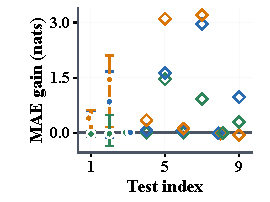
\includegraphics[width=\linewidth]{figs/input_form_gain_a.pdf}\subcaption{Full versus no-$D_0$}\end{subfigure}\hfill
\begin{subfigure}[t]{1.8in}\centering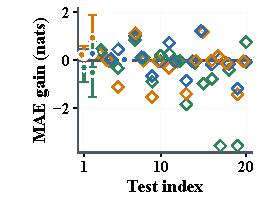
\includegraphics[width=\linewidth]{figs/input_form_gain_b.pdf}\subcaption{Source-free comparison}\end{subfigure}\hfill
\begin{subfigure}[t]{1.8in}\centering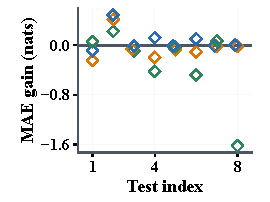
\includegraphics[width=\linewidth]{figs/input_form_gain_c.pdf}\subcaption{Power versus alternatives}\end{subfigure}

\caption{Paired improvements, zero line marked, positive means the first-named model is better. A: full model against its no-$D_0$ variant, per arm and capability; intervals only where a cluster bootstrap was computed (leave-one-stage-out panels), $n$ = evaluated source states. B: source-conditioned candidate against the strongest source-free baseline for all twenty registered tests (hollow = frozen prospective, filled = leave-one-out). C: shared power form against the same-input alternatives A1 and A2 on the pruning configuration tests. Generated by \texttt{plot\_fig2\_gains.py} from the frozen result files (Appendix J).}
\label{fig:gains}
\end{figure}

\FloatBarrier

\FloatBarrier

\section{Gradient-space analysis}
\label{sec:supp_gradient}

\subsection{Capabilities occupy distinct regions of gradient space}
\label{sec:regions}

\paragraph{Convergent validity (block structure).} For each of nine
benchmarks we measure a gradient signature (the benchmark-conditional
diagonal Fisher) and compare all pairs. After removing the component
shared across benchmarks, signatures of same-capability benchmarks are
positively aligned (cosine $+0.36$ to $+0.45$) while signatures of
different capabilities are \emph{anti-aligned} ($-0.23$ to $-0.25$),
in each of the ten models from five series for which the block analysis was run
(Figs.~\ref{fig:blocks}--\ref{fig:blocks_olmo3_7b}); the C4 control sits between blocks.\preliminary{point estimates; example-bootstrap, permutation and
prompt-stability tests are left to future work} The
mathematics benchmarks cluster regardless of format, and within-block
fine structure is consistent with benchmark content (SVAMP, grade-school word problems,
is the loosest member of the math block). A projected-gradient SVD
version gives the same result in subspace terms: principal-angle
similarity within capability exceeds cross-capability similarity by
$2$--$4\times$.

\begin{figure}[p]
\centering

\includegraphics[width=5.5in]{figs/v9_blocks_Qwen-Qwen3-0.6B_legend.pdf}\\[1pt]
\begin{subfigure}[t]{2.7in}\centering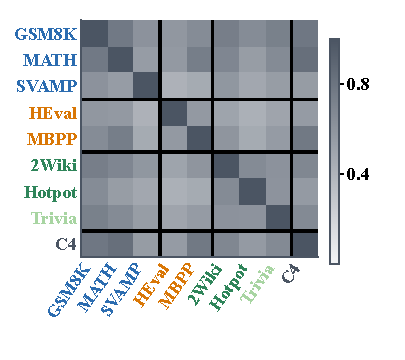
\includegraphics[width=\linewidth]{figs/v9_blocks_Qwen-Qwen3-0.6B_a.pdf}\subcaption{Raw Fisher cosine}\end{subfigure}
\hfill
\begin{subfigure}[t]{2.7in}\centering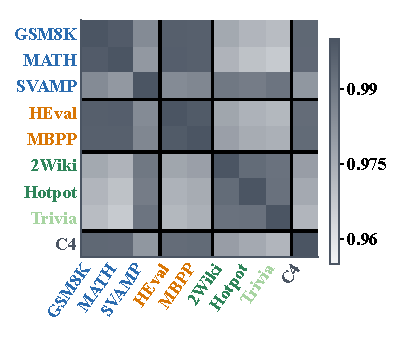
\includegraphics[width=\linewidth]{figs/v9_blocks_Qwen-Qwen3-0.6B_b.pdf}\subcaption{Log-Fisher cosine}\end{subfigure}
\\[3pt]
\begin{subfigure}[t]{2.7in}\centering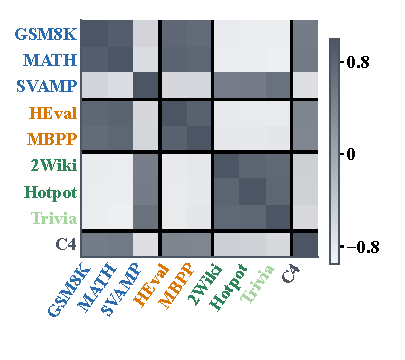
\includegraphics[width=\linewidth]{figs/v9_blocks_Qwen-Qwen3-0.6B_c.pdf}\subcaption{Residual log-Fisher cosine}\end{subfigure}
\hfill
\begin{subfigure}[t]{2.7in}\centering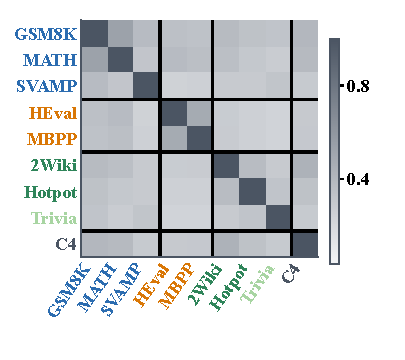
\includegraphics[width=\linewidth]{figs/v9_blocks_Qwen-Qwen3-0.6B_d.pdf}\subcaption{Top-0.1\% Jaccard}\end{subfigure}
\caption{Capability regions in gradient space for Qwen3-0.6B: pairwise similarity of per-benchmark gradient signatures under four metrics (raw Fisher cosine, log-Fisher cosine, shared-component-removed log-Fisher cosine, top-0.1\% coordinate Jaccard). Black lines separate the math, code, QA, and control blocks.}
\label{fig:blocks}
\label{fig:blocks_Qwen_Qwen3_06B}
\end{figure}

\begin{figure}[p]
\centering

\includegraphics[width=5.5in]{figs/v9_blocks_Qwen-Qwen3-1.7B_legend.pdf}\\[1pt]
\begin{subfigure}[t]{2.7in}\centering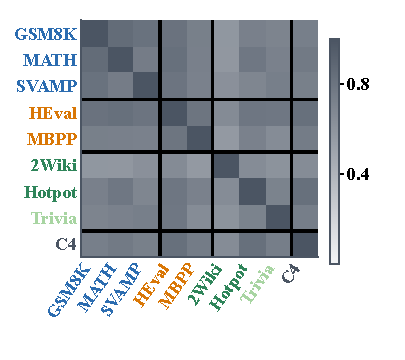
\includegraphics[width=\linewidth]{figs/v9_blocks_Qwen-Qwen3-1.7B_a.pdf}\subcaption{Raw Fisher cosine}\end{subfigure}
\hfill
\begin{subfigure}[t]{2.7in}\centering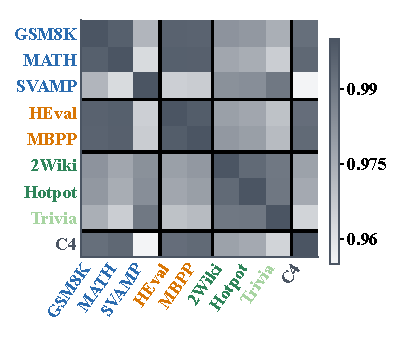
\includegraphics[width=\linewidth]{figs/v9_blocks_Qwen-Qwen3-1.7B_b.pdf}\subcaption{Log-Fisher cosine}\end{subfigure}
\\[3pt]
\begin{subfigure}[t]{2.7in}\centering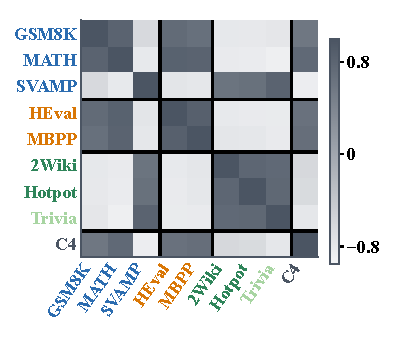
\includegraphics[width=\linewidth]{figs/v9_blocks_Qwen-Qwen3-1.7B_c.pdf}\subcaption{Residual log-Fisher cosine}\end{subfigure}
\hfill
\begin{subfigure}[t]{2.7in}\centering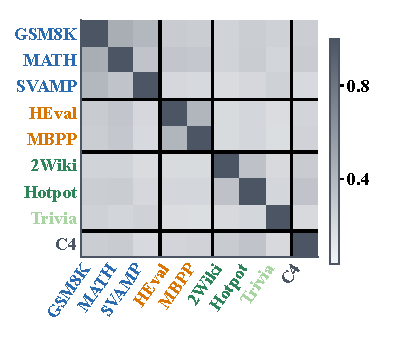
\includegraphics[width=\linewidth]{figs/v9_blocks_Qwen-Qwen3-1.7B_d.pdf}\subcaption{Top-0.1\% Jaccard}\end{subfigure}
\caption{Capability regions in gradient space for Qwen3-1.7B: pairwise similarity of per-benchmark gradient signatures under four metrics (raw Fisher cosine, log-Fisher cosine, shared-component-removed log-Fisher cosine, top-0.1\% coordinate Jaccard). Black lines separate the math, code, QA, and control blocks.}
\label{fig:blocks_Qwen_Qwen3_17B}
\end{figure}

\begin{figure}[p]
\centering

\includegraphics[width=5.5in]{figs/v9_blocks_Qwen-Qwen3-4B_legend.pdf}\\[1pt]
\begin{subfigure}[t]{2.7in}\centering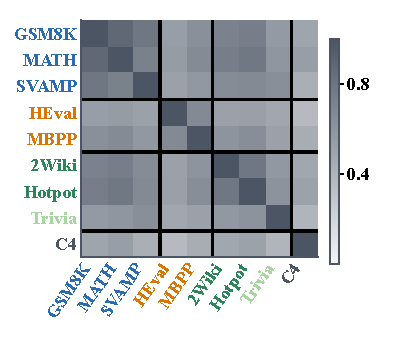
\includegraphics[width=\linewidth]{figs/v9_blocks_Qwen-Qwen3-4B_a.pdf}\subcaption{Raw Fisher cosine}\end{subfigure}
\hfill
\begin{subfigure}[t]{2.7in}\centering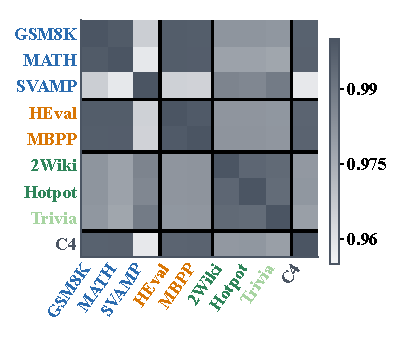
\includegraphics[width=\linewidth]{figs/v9_blocks_Qwen-Qwen3-4B_b.pdf}\subcaption{Log-Fisher cosine}\end{subfigure}
\\[3pt]
\begin{subfigure}[t]{2.7in}\centering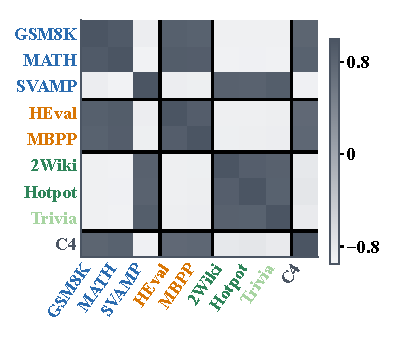
\includegraphics[width=\linewidth]{figs/v9_blocks_Qwen-Qwen3-4B_c.pdf}\subcaption{Residual log-Fisher cosine}\end{subfigure}
\hfill
\begin{subfigure}[t]{2.7in}\centering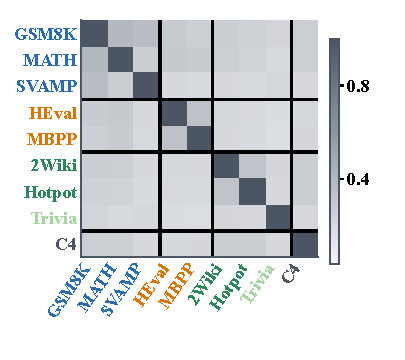
\includegraphics[width=\linewidth]{figs/v9_blocks_Qwen-Qwen3-4B_d.pdf}\subcaption{Top-0.1\% Jaccard}\end{subfigure}
\caption{Capability regions in gradient space for Qwen3-4B: pairwise similarity of per-benchmark gradient signatures under four metrics (raw Fisher cosine, log-Fisher cosine, shared-component-removed log-Fisher cosine, top-0.1\% coordinate Jaccard). Black lines separate the math, code, QA, and control blocks.}
\label{fig:blocks_Qwen_Qwen3_4B}
\end{figure}

\begin{figure}[p]
\centering

\includegraphics[width=5.5in]{figs/v9_blocks_gemma3-12b_legend.pdf}\\[1pt]
\begin{subfigure}[t]{2.7in}\centering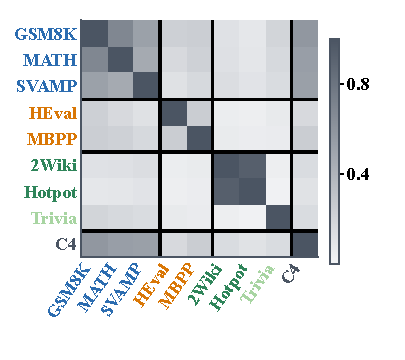
\includegraphics[width=\linewidth]{figs/v9_blocks_gemma3-12b_a.pdf}\subcaption{Raw Fisher cosine}\end{subfigure}
\hfill
\begin{subfigure}[t]{2.7in}\centering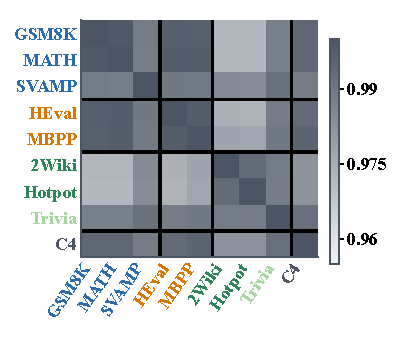
\includegraphics[width=\linewidth]{figs/v9_blocks_gemma3-12b_b.pdf}\subcaption{Log-Fisher cosine}\end{subfigure}
\\[3pt]
\begin{subfigure}[t]{2.7in}\centering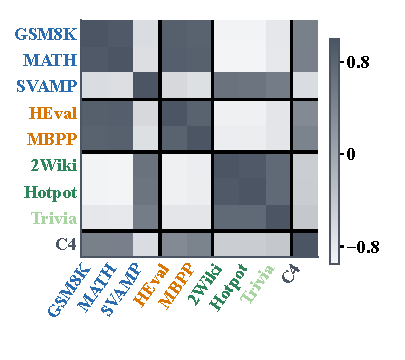
\includegraphics[width=\linewidth]{figs/v9_blocks_gemma3-12b_c.pdf}\subcaption{Residual log-Fisher cosine}\end{subfigure}
\hfill
\begin{subfigure}[t]{2.7in}\centering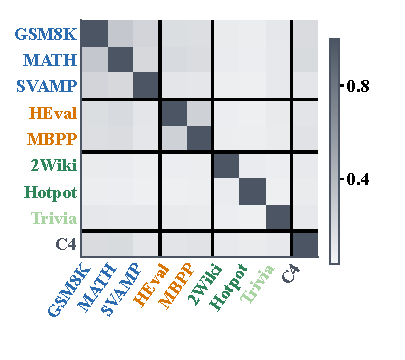
\includegraphics[width=\linewidth]{figs/v9_blocks_gemma3-12b_d.pdf}\subcaption{Top-0.1\% Jaccard}\end{subfigure}
\caption{Capability regions in gradient space for Gemma3-12B: pairwise similarity of per-benchmark gradient signatures under four metrics (raw Fisher cosine, log-Fisher cosine, shared-component-removed log-Fisher cosine, top-0.1\% coordinate Jaccard). Black lines separate the math, code, QA, and control blocks.}
\label{fig:blocks_gemma3_12b}
\end{figure}

\begin{figure}[p]
\centering

\includegraphics[width=5.5in]{figs/v9_blocks_gemma3-1b_legend.pdf}\\[1pt]
\begin{subfigure}[t]{2.7in}\centering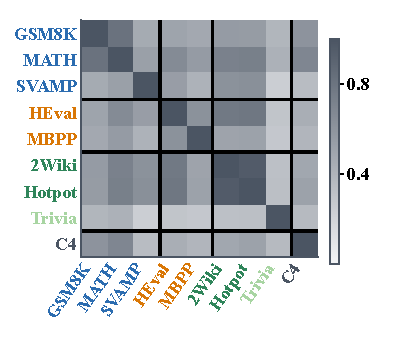
\includegraphics[width=\linewidth]{figs/v9_blocks_gemma3-1b_a.pdf}\subcaption{Raw Fisher cosine}\end{subfigure}
\hfill
\begin{subfigure}[t]{2.7in}\centering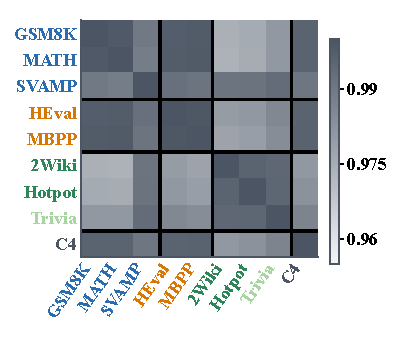
\includegraphics[width=\linewidth]{figs/v9_blocks_gemma3-1b_b.pdf}\subcaption{Log-Fisher cosine}\end{subfigure}
\\[3pt]
\begin{subfigure}[t]{2.7in}\centering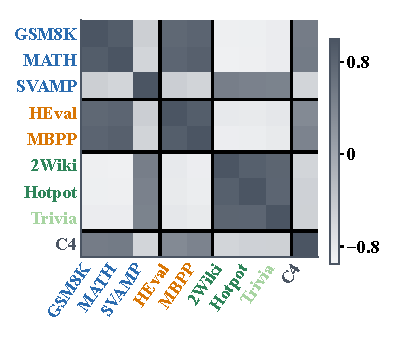
\includegraphics[width=\linewidth]{figs/v9_blocks_gemma3-1b_c.pdf}\subcaption{Residual log-Fisher cosine}\end{subfigure}
\hfill
\begin{subfigure}[t]{2.7in}\centering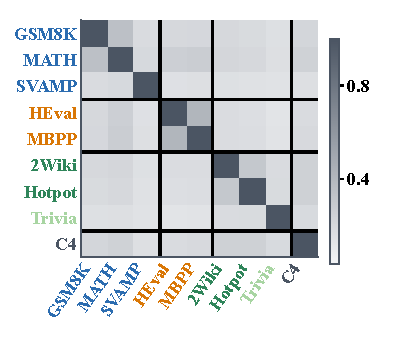
\includegraphics[width=\linewidth]{figs/v9_blocks_gemma3-1b_d.pdf}\subcaption{Top-0.1\% Jaccard}\end{subfigure}
\caption{Capability regions in gradient space for Gemma3-1B: pairwise similarity of per-benchmark gradient signatures under four metrics (raw Fisher cosine, log-Fisher cosine, shared-component-removed log-Fisher cosine, top-0.1\% coordinate Jaccard). Black lines separate the math, code, QA, and control blocks.}
\label{fig:blocks_gemma3_1b}
\end{figure}

\begin{figure}[p]
\centering

\includegraphics[width=5.5in]{figs/v9_blocks_gemma3-270m_legend.pdf}\\[1pt]
\begin{subfigure}[t]{2.7in}\centering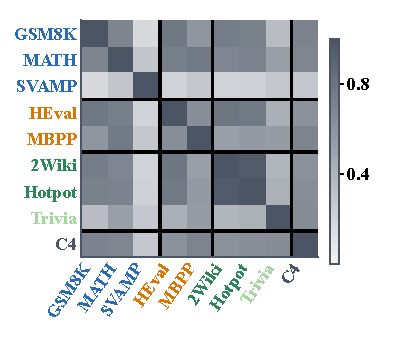
\includegraphics[width=\linewidth]{figs/v9_blocks_gemma3-270m_a.pdf}\subcaption{Raw Fisher cosine}\end{subfigure}
\hfill
\begin{subfigure}[t]{2.7in}\centering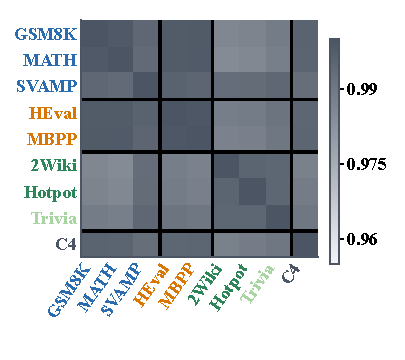
\includegraphics[width=\linewidth]{figs/v9_blocks_gemma3-270m_b.pdf}\subcaption{Log-Fisher cosine}\end{subfigure}
\\[3pt]
\begin{subfigure}[t]{2.7in}\centering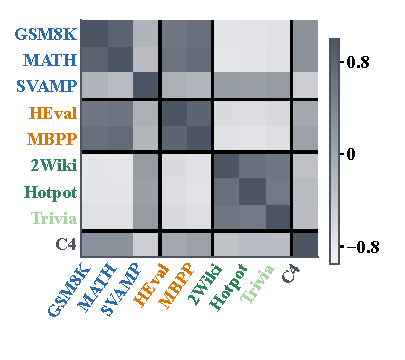
\includegraphics[width=\linewidth]{figs/v9_blocks_gemma3-270m_c.pdf}\subcaption{Residual log-Fisher cosine}\end{subfigure}
\hfill
\begin{subfigure}[t]{2.7in}\centering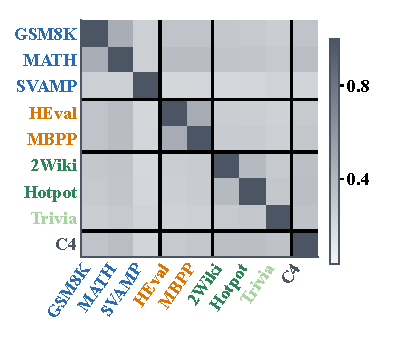
\includegraphics[width=\linewidth]{figs/v9_blocks_gemma3-270m_d.pdf}\subcaption{Top-0.1\% Jaccard}\end{subfigure}
\caption{Capability regions in gradient space for Gemma3-270M: pairwise similarity of per-benchmark gradient signatures under four metrics (raw Fisher cosine, log-Fisher cosine, shared-component-removed log-Fisher cosine, top-0.1\% coordinate Jaccard). Black lines separate the math, code, QA, and control blocks.}
\label{fig:blocks_gemma3_270m}
\end{figure}

\begin{figure}[p]
\centering

\includegraphics[width=5.5in]{figs/v9_blocks_gemma3-4b_legend.pdf}\\[1pt]
\begin{subfigure}[t]{2.7in}\centering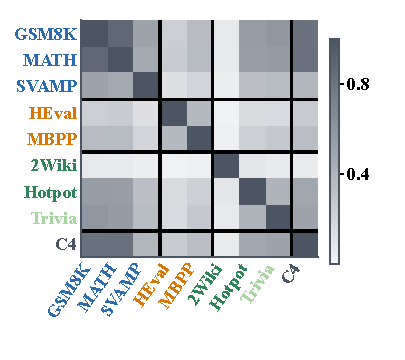
\includegraphics[width=\linewidth]{figs/v9_blocks_gemma3-4b_a.pdf}\subcaption{Raw Fisher cosine}\end{subfigure}
\hfill
\begin{subfigure}[t]{2.7in}\centering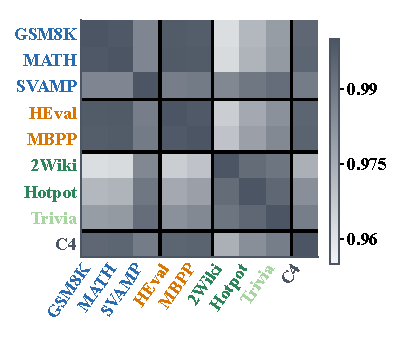
\includegraphics[width=\linewidth]{figs/v9_blocks_gemma3-4b_b.pdf}\subcaption{Log-Fisher cosine}\end{subfigure}
\\[3pt]
\begin{subfigure}[t]{2.7in}\centering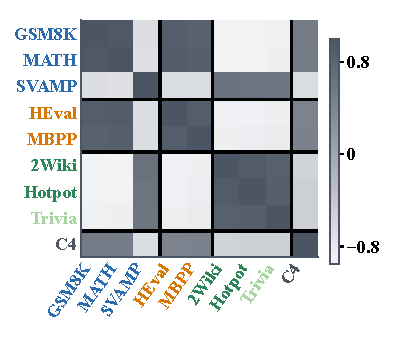
\includegraphics[width=\linewidth]{figs/v9_blocks_gemma3-4b_c.pdf}\subcaption{Residual log-Fisher cosine}\end{subfigure}
\hfill
\begin{subfigure}[t]{2.7in}\centering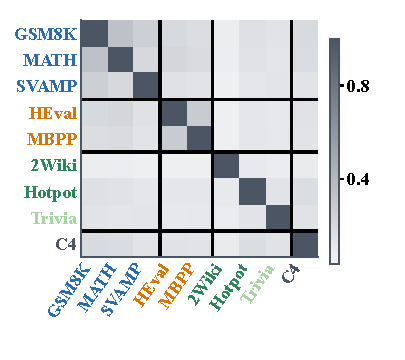
\includegraphics[width=\linewidth]{figs/v9_blocks_gemma3-4b_d.pdf}\subcaption{Top-0.1\% Jaccard}\end{subfigure}
\caption{Capability regions in gradient space for Gemma3-4B: pairwise similarity of per-benchmark gradient signatures under four metrics (raw Fisher cosine, log-Fisher cosine, shared-component-removed log-Fisher cosine, top-0.1\% coordinate Jaccard). Black lines separate the math, code, QA, and control blocks.}
\label{fig:blocks_gemma3_4b}
\end{figure}

\begin{figure}[p]
\centering

\includegraphics[width=5.5in]{figs/v9_blocks_gemma4-31b_legend.pdf}\\[1pt]
\begin{subfigure}[t]{2.7in}\centering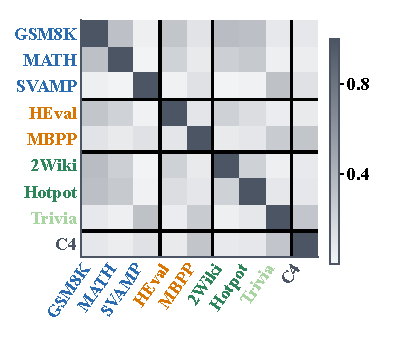
\includegraphics[width=\linewidth]{figs/v9_blocks_gemma4-31b_a.pdf}\subcaption{Raw Fisher cosine}\end{subfigure}
\hfill
\begin{subfigure}[t]{2.7in}\centering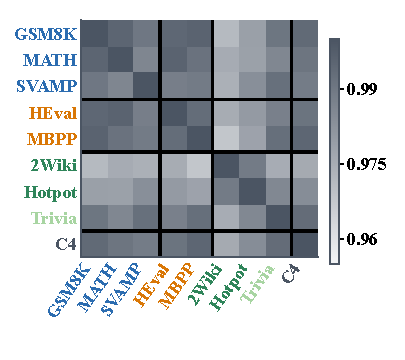
\includegraphics[width=\linewidth]{figs/v9_blocks_gemma4-31b_b.pdf}\subcaption{Log-Fisher cosine}\end{subfigure}
\\[3pt]
\begin{subfigure}[t]{2.7in}\centering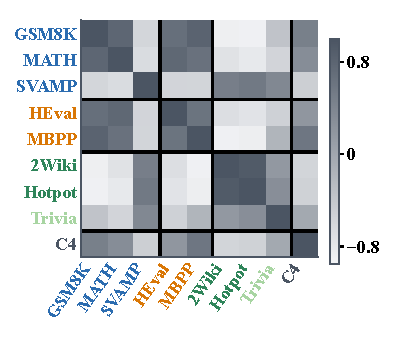
\includegraphics[width=\linewidth]{figs/v9_blocks_gemma4-31b_c.pdf}\subcaption{Residual log-Fisher cosine}\end{subfigure}
\hfill
\begin{subfigure}[t]{2.7in}\centering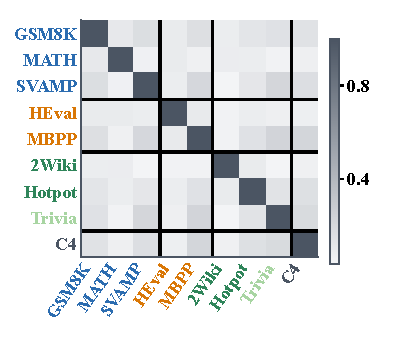
\includegraphics[width=\linewidth]{figs/v9_blocks_gemma4-31b_d.pdf}\subcaption{Top-0.1\% Jaccard}\end{subfigure}
\caption{Capability regions in gradient space for Gemma4-31B: pairwise similarity of per-benchmark gradient signatures under four metrics (raw Fisher cosine, log-Fisher cosine, shared-component-removed log-Fisher cosine, top-0.1\% coordinate Jaccard). Black lines separate the math, code, QA, and control blocks.}
\label{fig:blocks_gemma4_31b}
\end{figure}

\begin{figure}[p]
\centering

\includegraphics[width=5.5in]{figs/v9_blocks_muse-30b_legend.pdf}\\[1pt]
\begin{subfigure}[t]{2.7in}\centering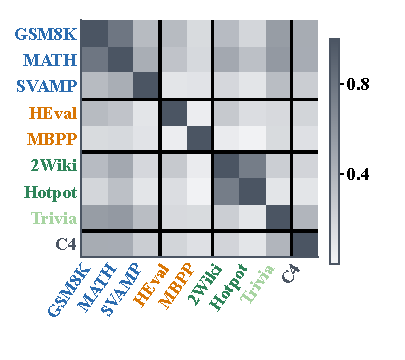
\includegraphics[width=\linewidth]{figs/v9_blocks_muse-30b_a.pdf}\subcaption{Raw Fisher cosine}\end{subfigure}
\hfill
\begin{subfigure}[t]{2.7in}\centering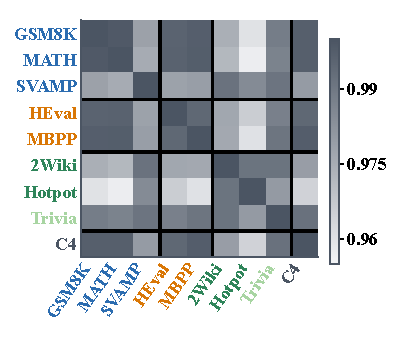
\includegraphics[width=\linewidth]{figs/v9_blocks_muse-30b_b.pdf}\subcaption{Log-Fisher cosine}\end{subfigure}
\\[3pt]
\begin{subfigure}[t]{2.7in}\centering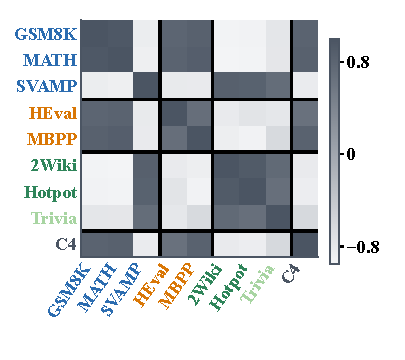
\includegraphics[width=\linewidth]{figs/v9_blocks_muse-30b_c.pdf}\subcaption{Residual log-Fisher cosine}\end{subfigure}
\hfill
\begin{subfigure}[t]{2.7in}\centering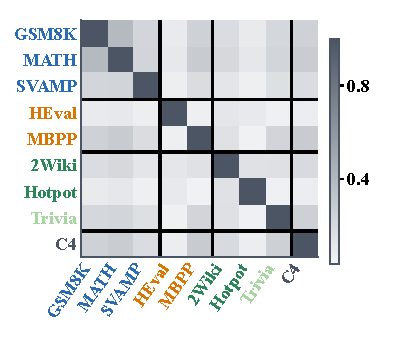
\includegraphics[width=\linewidth]{figs/v9_blocks_muse-30b_d.pdf}\subcaption{Top-0.1\% Jaccard}\end{subfigure}
\caption{Capability regions in gradient space for Muse-30B: pairwise similarity of per-benchmark gradient signatures under four metrics (raw Fisher cosine, log-Fisher cosine, shared-component-removed log-Fisher cosine, top-0.1\% coordinate Jaccard). Black lines separate the math, code, QA, and control blocks.}
\label{fig:blocks_muse_30b}
\end{figure}

\begin{figure}[p]
\centering

\includegraphics[width=5.5in]{figs/v9_blocks_olmo3-7b_legend.pdf}\\[1pt]
\begin{subfigure}[t]{2.7in}\centering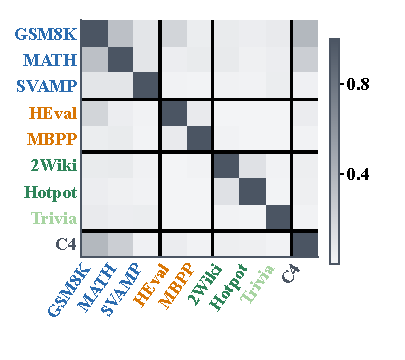
\includegraphics[width=\linewidth]{figs/v9_blocks_olmo3-7b_a.pdf}\subcaption{Raw Fisher cosine}\end{subfigure}
\hfill
\begin{subfigure}[t]{2.7in}\centering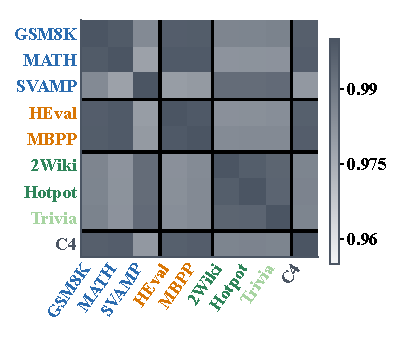
\includegraphics[width=\linewidth]{figs/v9_blocks_olmo3-7b_b.pdf}\subcaption{Log-Fisher cosine}\end{subfigure}
\\[3pt]
\begin{subfigure}[t]{2.7in}\centering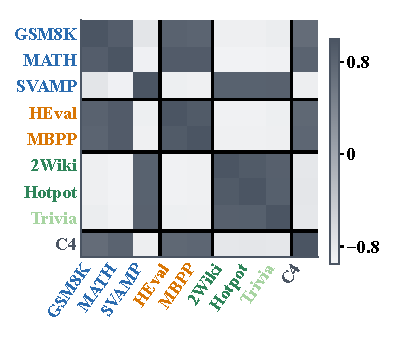
\includegraphics[width=\linewidth]{figs/v9_blocks_olmo3-7b_c.pdf}\subcaption{Residual log-Fisher cosine}\end{subfigure}
\hfill
\begin{subfigure}[t]{2.7in}\centering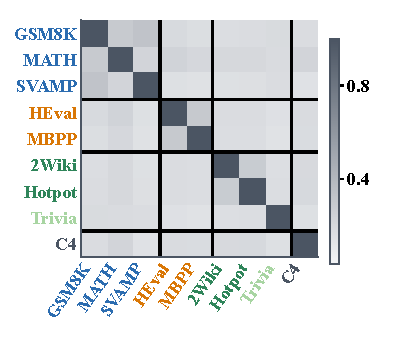
\includegraphics[width=\linewidth]{figs/v9_blocks_olmo3-7b_d.pdf}\subcaption{Top-0.1\% Jaccard}\end{subfigure}
\caption{Capability regions in gradient space for OLMo3-7B: pairwise similarity of per-benchmark gradient signatures under four metrics (raw Fisher cosine, log-Fisher cosine, shared-component-removed log-Fisher cosine, top-0.1\% coordinate Jaccard). Black lines separate the math, code, QA, and control blocks.}
\label{fig:blocks_olmo3_7b}
\end{figure}


\paragraph{Selective ablation.}\preliminary{single model; random, magnitude-matched and global-Fisher control ablations are left to future work} We
select the top $0.05\%$ of weight coordinates by each capability's
\emph{residual} Fisher signature (excluding coordinates shared with
other capabilities) and zero them. The damage matrix is nearly
diagonal (Gemma-3-1B; rows ablate, columns measure, nats/token):

\begin{center}
\small
\begin{tabular*}{\textwidth}{@{\extracolsep{\fill}}lrrr@{}}
\toprule
Ablated region & Math & Code & QA \\
\midrule
Math & $\mathbf{+4.63}$ & $+0.43$ & $+0.05$ \\
Code & $+0.42$ & $\mathbf{+7.14}$ & $+0.00$ \\
QA   & $+0.01$ & $+0.00$ & $\mathbf{+2.29}$ \\
\bottomrule
\end{tabular*}
\captionof*{table}{\mbox{Post-hoc} selective-ablation measurements. Rows identify the ablated capability region; columns identify the measured capability. Entries are loss increases in nats per native token; bold entries mark the matching capability.}
\end{center}

Zeroing $0.05\%$ of weights, selected from gradients alone, selectively
removes one capability while leaving the others nearly untouched
(the QA ablation moves code by $+0.0001$). Pending multi-model
replication and the control ablations above, we describe the regions as
causally implicated and partially separable; we do not call them proven
causal carriers; if confirmed, ablation itself is a form of
\emph{targeted} scaling-down.

\FloatBarrier

\FloatBarrier

\section{Selection addenda, recovery and earlier analyses}
\label{sec:supp_selection}

\begin{table}[H]
\centering\small
\setlength{\tabcolsep}{3pt}
\caption{V78 regret by source state and objective. Each entry is the mean over all 17 nominal storage budgets (0.20--1.00, step 0.05), in nats. $K$ counts distinct configurations selected by the Frozen selection rule across these budgets.}
\label{tab:rule-confirm-by-state}
\begin{tabular}{llrrrrr}
\toprule
State & Objective & \shortstack{Frozen selection\\rule} & \shortstack{Source-conditioned\\predictor} & Quantization-only & \shortstack{Cheapest\\feasible} & $K$ \\
\midrule
160M @ 32k & Math & 0.000000 & 0.000512 & 0.000035 & 2.902545 & 7 \\
 & Code & 0.000000 & 0.000000 & 0.000035 & 3.767303 & 7 \\
 & QA (2Wiki) & 0.220466 & 0.141708 & 0.126440 & 1.882328 & 4 \\
 & Multi & 0.001169 & 0.003603 & 0.001204 & 3.764622 & 7 \\
\midrule
410M @ 32k & Math & 0.000000 & 0.028442 & 0.000009 & 1.607308 & 7 \\
 & Code & 0.001014 & 0.410475 & 0.000923 & 2.053675 & 7 \\
 & QA (2Wiki) & 0.046997 & 0.183243 & 0.216010 & 1.459195 & 4 \\
 & Multi & 0.002180 & 0.001677 & 0.002334 & 2.050533 & 7 \\
\midrule
1.4B @ 32k & Math & 0.000024 & 0.030380 & 0.000000 & 2.248675 & 7 \\
 & Code & 0.011972 & 0.013315 & 0.012025 & 3.526863 & 7 \\
 & QA (2Wiki) & 0.244136 & 0.523932 & 0.387497 & 2.013168 & 4 \\
 & Multi & 0.004743 & 0.002122 & 0.005323 & 3.507343 & 7 \\
\midrule
1B @ 64k & Math & 0.000000 & 0.000434 & 0.026970 & 0.327902 & 7 \\
 & Code & 0.004321 & 0.025644 & 0.027814 & 0.390606 & 7 \\
 & QA (2Wiki) & 0.052428 & 0.005406 & 0.280362 & 0.052428 & 1 \\
 & Multi & 0.000000 & 0.000000 & 0.023494 & 0.382624 & 7 \\
\bottomrule
\end{tabular}
\par\smallskip\begin{minipage}{\linewidth}\footnotesize
All four policies are feasible on all 68 state--budget cells per objective. Multi minimizes $\max_c[L_c(M)-L_c(M_0)]$. QA uses 2Wiki. The 1B/64k state includes two historical V39 KD students, excluded from the V78 prediction fits. Policy internal names: locked-rule, v64-law (respectively).
\end{minipage}
\end{table}

\begin{table}[H]
\centering\small
\setlength{\tabcolsep}{3pt}
\caption{Heuristic candidate-set sizes and oracle coverage on all 68 cells per objective. Size columns count methods in the no-clear-winner candidate set, including singleton sets. Both coverage columns describe the set, not the single choice, and report count/68 (percent).}
\label{tab:rule-confirm-candidate-sizes}
\begin{tabularx}{\linewidth}{lXrrrrrr}
\toprule
& & \multicolumn{4}{c}{Set size (methods)} & \multicolumn{2}{c}{Oracle coverage} \\
\cmidrule(lr){3-6}\cmidrule(lr){7-8}
Objective & Policy & 1 & 2 & 3 & 4 & \shortstack{Set contains\\oracle method} & \shortstack{Set contains\\oracle configuration} \\
\midrule
Math & Frozen selection rule & 30 & 28 & 10 & 0 & 68/68 (100.0) & 68/68 (100.0) \\
 & Source-conditioned predictor & 31 & 27 & 10 & 0 & 68/68 (100.0) & 39/68 (57.4) \\
\midrule
Code & Frozen selection rule & 30 & 28 & 10 & 0 & 68/68 (100.0) & 37/68 (54.4) \\
 & Source-conditioned predictor & 30 & 26 & 11 & 1 & 68/68 (100.0) & 23/68 (33.8) \\
\midrule
QA (2Wiki) & Frozen selection rule & 24 & 32 & 12 & 0 & 68/68 (100.0) & 18/68 (26.5) \\
 & Source-conditioned predictor & 26 & 30 & 12 & 0 & 66/68 (97.1) & 23/68 (33.8) \\
\midrule
Multi & Frozen selection rule & 30 & 28 & 10 & 0 & 68/68 (100.0) & 54/68 (79.4) \\
 & Source-conditioned predictor & 32 & 26 & 10 & 0 & 68/68 (100.0) & 62/68 (91.2) \\
\bottomrule
\end{tabularx}
\par\smallskip\begin{minipage}{\linewidth}\footnotesize
Sets reuse frozen development LOSO MAE thresholds; coverage is retrospective, not calibrated uncertainty. On this panel the no-clear-winner flag holds exactly for sets of size $\geq2$. The Source-conditioned predictor for Code at 1B/64k and budget 1.00 has four candidates (quantization, dense, pruning, distillation); it is retained explicitly. Set contains oracle method tests whether the measured oracle's method belongs to the candidate methods. Set contains oracle configuration tests whether its exact configuration ID belongs to the set of one predicted best configuration per included method. Neither column tests the single selected configuration. Policy internal names: locked-rule, v64-law (respectively).
\end{minipage}
\end{table}

\begin{table}[H]
\setbox2=\vbox{\begin{minipage}{\linewidth}
\centering
\small
\setlength{\tabcolsep}{3pt}
\caption{The table inventories measured candidate coverage by source state. Each method column gives configuration count followed by the minimum available storage ratio $r$. Rows identify source states; columns give availability by compression method and the minimum quantization storage ratio. Counts are numbers of configurations and storage ratios are dimensionless. This is a \mbox{post-hoc} inventory of the development selection panel.}
\label{tab:candidate-coverage}
\setbox0=\hbox{
\begin{tabular}{lrrrrr}
\toprule
Source state & Pruning & \shortstack[l]{Per-channel\\round-to-nearest\\quantization} & \shortstack[l]{Grouped\\round-to-nearest\\quantization} & \shortstack[l]{distillation\\students} & \shortstack[l]{Minimum quantization\\storage ratio} \\
\midrule
\shortstack[l]{Pythia-160M at step\\16k} & 4; 0.6000000 & 4; 0.1875000 & 9; 0.1914062 & 0; not available & 0.1875000 \\
\shortstack[l]{Pythia-160M at step\\64k} & 4; 0.6000000 & 4; 0.1875000 & 0; not available & 0; not available & 0.1875000 \\
\shortstack[l]{Pythia-160M at step\\96k} & 4; 0.6000000 & 4; 0.1875000 & 0; not available & 0; not available & 0.1875000 \\
\shortstack[l]{Pythia-160M at step\\143k} & 6; 0.5500000 & 4; 0.1875000 & 9; 0.1914062 & 0; not available & 0.1875000 \\
\shortstack[l]{Pythia-410M at step\\16k} & 4; 0.6000000 & 4; 0.1875000 & 9; 0.1914062 & 1; 0.2812500 & 0.1875000 \\
\shortstack[l]{Pythia-410M at step\\64k} & 4; 0.6000000 & 4; 0.1875000 & 0; not available & 1; 0.2812500 & 0.1875000 \\
\shortstack[l]{Pythia-410M at step\\96k} & 6; 0.5500000 & 4; 0.1875000 & 0; not available & 0; not available & 0.1875000 \\
\shortstack[l]{Pythia-410M at step\\143k} & 4; 0.6000000 & 4; 0.1875000 & 9; 0.1914062 & 1; 0.2812500 & 0.1875000 \\
\shortstack[l]{Pythia-1B at step\\32k} & 7; 0.5500000 & 5; 0.1875000 & 0; not available & 0; not available & 0.1875000 \\
\shortstack[l]{Pythia-1B at step\\96k} & 2; 0.5500000 & 2; 0.1875000 & 3; 0.1953125 & 0; not available & 0.1875000 \\
\shortstack[l]{Pythia-1B at step\\112k} & 7; 0.5500000 & 5; 0.1875000 & 0; not available & 0; not available & 0.1875000 \\
\shortstack[l]{Pythia-1.4B at step\\16k} & 4; 0.6000000 & 4; 0.1875000 & 9; 0.1914062 & 2; 0.0703125 & 0.1875000 \\
\shortstack[l]{Pythia-1.4B at step\\64k} & 6; 0.5500000 & 4; 0.1875000 & 0; not available & 2; 0.0703125 & 0.1875000 \\
\shortstack[l]{Pythia-1.4B at step\\96k} & 4; 0.6000000 & 4; 0.1875000 & 0; not available & 0; not available & 0.1875000 \\
\shortstack[l]{Pythia-1.4B at step\\143k} & 4; 0.6000000 & 4; 0.1875000 & 9; 0.1914062 & 2; 0.0703125 & 0.1875000 \\
\shortstack[l]{Pythia-6.9B at step\\32k} & 7; 0.5500000 & 5; 0.1875000 & 0; not available & 0; not available & 0.1875000 \\
\shortstack[l]{Pythia-6.9B at step\\112k} & 7; 0.5500000 & 5; 0.1875000 & 0; not available & 0; not available & 0.1875000 \\
\midrule
Total & 84 & 70 & 57 & 9 & --- \\
\bottomrule
\end{tabular}
}\ifdim\wd0>\linewidth\resizebox{\linewidth}{!}{\box0}\else\box0\fi
\par\smallskip
\begin{minipage}{\linewidth}\small
Not available means no measured candidate. Each state also has one dense source, minimum $r=1$; it is excluded from method counts. Distillation has 0, 1 or 2 smaller same-stage measured students. Student reuse across sources counts as separate alternatives, not independent measurements. Quantization pools channel and grouped round-to-nearest quantization. Ratios: pruning $r=d$, channel round-to-nearest quantization $r=b/16$, grouped round-to-nearest quantization $r=(b+16/g)/16$, distillation $r=N_S/N_0$. Storage is nominal transformer-matrix storage; pruning requires a sparse format (index overhead excluded). No missing configurations are imputed. Coverage is measured availability, independent of the no-clear-winner heuristic.
\end{minipage}
\end{minipage}}
\centering\ifdim\dimexpr\ht2+\dp2\relax>.95\textheight\resizebox*{!}{.95\textheight}{\box2}\else\box2\fi
\end{table}

\FloatBarrier

\paragraph{Resource-ratio models.} A method-agnostic response in the
storage or active-parameter ratio was tested on the heterogeneous
panel: at the common storage ratio $0.5$, pruning to $d=0.5$ costs
median $+5.9$, $+8.2$, and $+2.9$ nats while int8 quantization costs
none; over 75 storage-matched pairs (14 with both sides pre-cliff) the
mean absolute method gap is $9.3$ nats with sign agreement $0.61$, and
the two shared-law hypotheses fit on pre-cliff cells reach held-out
sign accuracies of $0.51$ and $0.37$. These models are rejected;
whether another single form could unify the arms is untested. A
capability- and cost-aware method selection would use predictors like
these as loss constraints; the offline replay with frozen predictions
below quantifies the decision cost of prediction error on the
heterogeneous panel, and the held-out selection validation on the
Pythia panel is in Section 7 of the main paper and
Appendix H.

\subsection{Recovery arm: redeemable damage and the fitted plateau}
\label{sec:recovery}
\label{sec:app_recovery}

Recovery training on general text fits the recovery law cleanly
(Gemma3-270M pruned to $\dens=0.6$; $R^2\approx1.0$):
$\beta'_{\text{math}}=1.23$, $\beta'_{\text{code}}=1.02$, with
fitted plateaus under the fixed LoRA recipe and the largest measured
budget of 16M tokens, $\Lc{c}^{\text{plateau}}-\Lc{c}^{\text{dense}}$,
of $1.21$ (math) and $1.93$ (code) nats; about $80\%$ of this pruning
damage is redeemed within 8M tokens and the remainder persists up to
the largest budget measured under this recipe, while QA recovers
completely. The plateau is a fitted quantity at 16M tokens, not an
established asymptote, and the saturating form does not describe the
non-monotone aligned-data trajectory below. \preliminary{one model, one density, one recipe; with three-point
ladders the largest-budget extrapolation of the saturating form beats a
carry-forward baseline in only 4 of 9 fits, so the ladder is too sparse
to claim extrapolation, and a denser multi-model grid is left to future work} Two further results bear on mechanism.
Recovery on \emph{aligned} data (teacher traces) heals substantially
faster at small budgets (math $2.76$ vs.\ $3.47$ at $0.5$M tokens),
as the gradient-overlap prediction requires, but over-training on
narrow aligned data damages the model again (QA $4.95\to9.75$
from $0.5$M to $8$M tokens), while general-text recovery is monotone. Quantization damage past the bit cliff is markedly less redeemable
under the same recipe (residuals $\approx2.6$--$2.8$ after int3) than
pruning damage at matched severity.

\subsection{Re-analysis of an earlier ability-space grid}
\label{sec:app_cross}

A prior internal study fit compression laws directly on Rasch
abilities from $\sim$100-item panels over a 774-cell Qwen3 grid and
reported that no derived law had held-out predictive power. Our
re-analysis attributes much of this to the measurement layer:
(1) the $r{=}1$ falsification anchor was driven almost entirely by the
answer-only recipe (stratified, the anchor holds and held-out error
drops from $9.0\times$ to $1.8\times$ the noise floor); (2)
same-benchmark evaluation inflated QA gains by roughly one third;
(3) discrimination heterogeneity voids interval-scale ability while
rankings survive ($\rho\ge0.98$); (4) item-level damage is smooth
pre-cliff, ruling out discrete skill deletion at the item level.
These findings fixed the protocol of Section 2.1 of the main paper.

\FloatBarrier

\FloatBarrier
\paragraph{Feasible-policy results and rule decomposition.} The per-policy results behind the feasibility figure of Appendix~H of the main paper, and the decomposition of the locked rule's regret by state and budget, follow.
\begin{table}[!htbp]\normalfont
\centering
\small
\setlength{\tabcolsep}{3pt}
\caption{The table compares selection policies on their feasible compression choices. Coverage and agreement with the measured oracle are percentages; mean regret is in nats per native token. Results distinguish each policy's feasible cells from the cells shared by all policies.}
\label{tab:selection-feasible}
\begin{tabular*}{\textwidth}{@{\extracolsep{\fill}}>{\raggedright\arraybackslash\hspace{0pt}}p{\dimexpr 0.220000000\textwidth-2.640000000\tabcolsep\relax}>{\raggedright\arraybackslash\hspace{0pt}}p{\dimexpr 0.190000000\textwidth-2.280000000\tabcolsep\relax}>{\raggedright\arraybackslash\hspace{0pt}}p{\dimexpr 0.100000000\textwidth-1.200000000\tabcolsep\relax}>{\raggedright\arraybackslash\hspace{0pt}}p{\dimexpr 0.120000000\textwidth-1.440000000\tabcolsep\relax}>{\raggedright\arraybackslash\hspace{0pt}}p{\dimexpr 0.120000000\textwidth-1.440000000\tabcolsep\relax}>{\raggedright\arraybackslash\hspace{0pt}}p{\dimexpr 0.120000000\textwidth-1.440000000\tabcolsep\relax}>{\raggedright\arraybackslash\hspace{0pt}}p{\dimexpr 0.130000000\textwidth-1.560000000\tabcolsep\relax}@{}}
\toprule
Policy & Objective & Coverage & \multicolumn{2}{>{\centering\arraybackslash\hspace{0pt}}p{\dimexpr 0.240000000\textwidth-0.880000000\tabcolsep\relax}}{Regret (nats)} & \multicolumn{2}{>{\centering\arraybackslash\hspace{0pt}}p{\dimexpr 0.250000000\textwidth-1.000000000\tabcolsep\relax}@{}}{Agreement (percent)} \\
\cmidrule(lr){4-5}\cmidrule(lr){6-7}
 & & (percent) & Policy-feasible cells & Shared feasible cells & Policy-feasible cells & Shared feasible cells \\
\midrule
Predicted selection & Math & 100.0 & 0.1936 & 0.2018 & 95.8 & 94.5 \\
Predicted selection & Code & 100.0 & 0.1743 & 0.1112 & 94.8 & 96.4 \\
Predicted selection & QA & 100.0 & 0.4184 & 0.1578 & 73.4 & 67.3 \\
Predicted selection & {Maximum across capabilities} & 100.0 & 0.0288 & 0.0174 & 93.8 & 94.5 \\
\midrule
Measured oracle & Math & 100.0 & 0.0000 & 0.0000 & 100.0 & 100.0 \\
Measured oracle & Code & 100.0 & 0.0000 & 0.0000 & 100.0 & 100.0 \\
Measured oracle & QA & 100.0 & 0.0000 & 0.0000 & 100.0 & 100.0 \\
Measured oracle & {Maximum across capabilities} & 100.0 & 0.0000 & 0.0000 & 100.0 & 100.0 \\
\midrule
Pruning only & Math & 55.7 & 0.5875 & 0.2896 & 0.0 & 0.0 \\
Pruning only & Code & 55.7 & 0.6218 & 0.3098 & 5.0 & 0.0 \\
Pruning only & QA & 55.7 & 0.7245 & 0.4469 & 44.1 & 9.1 \\
Pruning only & {Maximum across capabilities} & 55.7 & 0.6731 & 0.3295 & 1.2 & 0.0 \\
\midrule
Quantization only & Math & 100.0 & 0.2089 & 0.2018 & 96.5 & 92.7 \\
Quantization only & Code & 100.0 & 0.1943 & 0.1112 & 94.1 & 96.4 \\
Quantization only & QA & 100.0 & 0.4905 & 0.5735 & 47.8 & 7.3 \\
Quantization only & {Maximum across capabilities} & 100.0 & 0.0428 & 0.0178 & 93.1 & 90.9 \\
\midrule
Distillation only & Math & 33.2 & 0.2968 & 0.3225 & 1.0 & 0.0 \\
Distillation only & Code & 33.2 & 0.3366 & 0.3626 & 3.1 & 0.0 \\
Distillation only & QA & 33.2 & 0.0564 & 0.0665 & 83.3 & 83.6 \\
Distillation only & {Maximum across capabilities} & 33.2 & 0.3332 & 0.3606 & 3.1 & 0.0 \\
\midrule
{Cheapest feasible configuration} & Math & 100.0 & 4.5839 & 2.0931 & 79.9 & 43.6 \\
{Cheapest feasible configuration} & Code & 100.0 & 5.1745 & 2.2502 & 78.9 & 47.3 \\
{Cheapest feasible configuration} & QA & 100.0 & 4.3334 & 1.8392 & 64.7 & 58.2 \\
{Cheapest feasible configuration} & {Maximum across capabilities} & 100.0 & 5.1782 & 2.2700 & 78.2 & 43.6 \\
\bottomrule
\end{tabular*}
\par\smallskip
\begin{minipage}{\linewidth}\small
Coverage is feasible cells / 289. Own averages only that policy's feasible cells; common averages the same 55/289 cells feasible for all six policies, including Cheapest feasible configuration. Agreement uses those same respective subsets. Empty subsets are marked not available. An empty candidate set returns infeasible with no source fallback. Dense ($r=1$) is eligible for predicted selection, measured oracle, and cheapest feasible configuration only at $r_{\max}=1$. Fixed policies retain only their named method; Quantization only pools channel and grouped round-to-nearest quantization. Each deployed endpoint is an absolute loss: source dense plus response for pruning and round-to-nearest quantization; student dense plus student post-training change for distillation. The maximum-capability objective is $\max_c(L_c-L_{0c})$. The unchanged no-clear-winner heuristic uses pooled leave-one-state-out mean absolute errors and is not calibrated uncertainty. Five-bit folds remain underidentified; measurement coverage and dense anchors vary by arm.
\end{minipage}
\end{table}

% Generated by analysis/v85_selection_decomp.py; original V78 cell regrets.
\begin{table}[H]
\centering\small
\setlength{\tabcolsep}{4pt}\renewcommand{\arraystretch}{1.08}
\begin{tabular}{@{}llrrr@{}}
\toprule
Objective & Policy & Step-32k & 1B@64k & All states \\
 & Cells per objective & 51 & 17 & 68 \\
\midrule
Math & Frozen rule & 0.000008 & 0.000000 & 0.000006 \\
 & Source-conditioned predictor & 0.019778 & 0.000434 & 0.014942 \\
 & Quantization-only & 0.000015 & 0.026970 & 0.006754 \\
 & Cheapest & 2.252843 & 0.327902 & 1.771608 \\
 & Frozen minus quant. & -0.000007 & -0.026970 & -0.006748 \\
\addlinespace
Code & Frozen rule & 0.004329 & 0.004321 & 0.004327 \\
 & Source-conditioned predictor & 0.141263 & 0.025644 & 0.112358 \\
 & Quantization-only & 0.004328 & 0.027814 & 0.010199 \\
 & Cheapest & 3.115947 & 0.390606 & 2.434612 \\
 & Frozen minus quant. & +0.000001 & -0.023494 & -0.005873 \\
\addlinespace
QA & Frozen rule & 0.170533 & 0.052428 & 0.141007 \\
 & Source-conditioned predictor & 0.282961 & 0.005406 & 0.213573 \\
 & Quantization-only & 0.243316 & 0.280362 & 0.252577 \\
 & Cheapest & 1.784897 & 0.052428 & 1.351780 \\
 & Frozen minus quant. & -0.072783 & -0.227934 & -0.111571 \\
\addlinespace
Multi (max) & Frozen rule & 0.002697 & 0.000000 & 0.002023 \\
 & Source-conditioned predictor & 0.002467 & 0.000000 & 0.001850 \\
 & Quantization-only & 0.002954 & 0.023494 & 0.008089 \\
 & Cheapest & 3.107499 & 0.382624 & 2.426280 \\
 & Frozen minus quant. & -0.000256 & -0.023494 & -0.006066 \\
\bottomrule
\end{tabular}
\caption{Selection regret decomposition (native-token nats; lower is better). Step-32k comprises 160M, 410M, and 1.4B: pruning and quantization candidates with newly measured outcomes. 1B@64k additionally includes two historical distillation candidates. The original dense candidate is retained at budget 1.0 in every state. Means weight each state--budget cell equally over 17 storage budgets (0.20--1.00 in steps of 0.05); all-state means weight the subsets 3:1. Quantization-only pools per-channel and grouped candidates using frozen-rule predictions. Multi minimizes $\max_c(L_c-L_{0,c}^{\mathrm{source}})$. Differences are computed before rounding; negative favors the frozen rule.}
\label{tab:rule_decomp}
\end{table}

\FloatBarrier
